% NE 630 -- Lesson 22. Only this lesson has migrated to the unified class.
% Build: make L22 (XeLaTeX; no shell escape or Python needed for the PDF).
% Slide coverage and editorial corrections: handout_backend.md.
\documentclass{ne630handout}
\handoutsolutionsfalse
\hypersetup{pdftitle={NE 630 -- Lesson 22: Reactivity impacts of xenon and samarium},
  pdfauthor={Jeremy Roberts},pdfsubject={Fission-product reactivity and the iodine--xenon transient}}
\begin{document}
\Lesson{22}{Reactivity impacts of xenon and samarium}
 {FNRP \S\,10.1--10.3; Eqs.\ (10.4), (10.7), and (10.12)--(10.13).}
 { }
\textbf{Objective:} \Primary{Quantify the impact of xenon and samarium buildup on reactivity.}

% Column pattern: \colstart (left), \colnext (right), \colend (finish pair).
% Close any box environment before switching/ending columns or starting a page.
\colstart
\Sec{1}{Review: reactivity}
The multiplication factor ($k$) and reactivity ($\rho$) are related by
\[
 \rho=\frac{k-1}{k} \qquad \text{and} \qquad k=\frac{1}{1-\rho}.
\]
Reactivity is given in $\Delta k/k$, $\%\,\Delta k/k$, pcm, or dollars.
Changes are characterized by \textbf{(integral) worths}, $\Delta\rho$, and
\textbf{reactivity coefficients},
\[
 \alpha_x=\left.\frac{\partial\rho}{\partial x}\right|_{\text{non-}x\text{ fixed}}.
\]
 
%%%%%%%%%%%%%%%%%%%%%%%%%%%%%%%%%%%%%%%%%%%%%%%%%%%%%%%%%%%%%%%%%%%%%%%%%%%%%%%
\Sec{2}{Reactivity in time}

As a reactor operates at power, its excess reactivity typically
\emph{decreases} because \Primary{\nucl{235}{U} is consumed} and
\Primary{parasitic fission products (FPs) are born}. That excess reactivity
must \Alert{be balanced by control}.

\vspace{5pt}

To represent these processes, define a time-varying multiplication factor as
\begin{equation*}
 k(t)=\frac{\Primary{\nu\bar\Sigma_{fT}^F(t)}\,p\,\varepsilon\,P_{\rm NL}}
 {\bar\Sigma_{aT}^F(t)+\Primary{\bar\Sigma_{aT}^{\rm FP}(t)}
  +\varsigma\dfrac{V_M}{V_F}
   \left[\bar\Sigma_{aT}^{M}+\Alert{\bar\Sigma_{aT}^{\rm control}(t)}\right]} \, ,
 \tag{FNRP 10.4*}
\end{equation*}
where $P_{\text{NL}}$ is the probability that neutrons do not leak from the system.  

\vspace{5pt}

During operation, \Alert{$\bar\Sigma_{aT}^{\rm control}(t)$} must be adjusted
to maintain $k(t)=1$. This model places \Alert{adjustable control} in the
moderator volume, consistent with typical LWRs, whether by way  
of changing \Alert{rod position} or the \Alert{soluble poison concentration}.

%%%%%%%%%%%%%%%%%%%%%%%%%%%%%%%%%%%%%%%%%%%%%%%%%%%%%%%%%%%%%%%%%%%%%%%%%%%%%%%
\Sec{3}{Fission products and fission yields}
Fission of \nucl{235}{U} (or \nucl{239}{Pu}, \ldots) produces two massive
fragments called \textbf{fission products}. Often, FPs are
\begin{itemize}
 \item \emph{radioactive} (which decay modes dominate?);
 \item \emph{parasitic neutron absorbers} with large $\sigma_a$ (thermal and/or
       epithermal).
\end{itemize}
The \textbf{fission yield}, $\gamma_{\text{fp}}$, specifies the production of a
given FP per fission.
\begin{center}
\begin{tabular}{@{}lrlr@{}}
\toprule
Nuclide & $\gamma_{\text{fp}}$ & Nuclide & $\gamma_{\text{fp}}$\\
\midrule
\nucl{134}{Xe} & $0.078$ & \nucl{137}{Cs} & $0.063$\\
\nucl{133}{Cs} & $0.067$ & \nucl{135}{I} & $0.063$\\
\nucl{95}{Mo}  & $0.065$ & \nucl{99}{Tc} & $0.061$\\
\bottomrule
\end{tabular}
\end{center}
\figcap{Selected \nucl{235}{U} yields from the IAEA WIMS Library Update project.}

\vspace{5pt}

\textbf{Ponderable:} 
{\large $\sum_{\text{fp}\,\in\,\text{all FPs}}\gamma_{\text{fp}} = \mathbf{?}$}
 
\colnext

%%%%%%%%%%%%%%%%%%%%%%%%%%%%%%%%%%%%%%%%%%%%%%%%%%%%%%%%%%%%%%%%%%%%%%%%%%%%%%%
\Sec{4}{Evolution of FP concentrations}

For a FP produced directly from fission, production competes with
radioactive decay and neutron absorption:
\begin{align*}
 \frac{dN_{\text{fp}}}{dt}
  =-\lambda_{\text{fp}}N_{\text{fp}}(t) 
   -\overbrace{\bar\sigma_a^{\text{fp}}N_{\text{fp}}(t)}^{\bar\Sigma_a^{\text{fp}}(t)}\phi
       +\gamma_{\text{fp}}\bar\Sigma_f\phi ,
\tag{FNRP 10.7}
\end{align*}
where, as usual, the $\bar{\phantom{\sigma}}$ means spectrum averaging 
over \emph{all energies}, i.e.,
\[
 \bar\sigma_a^{\text{fp}}=
 \frac{\displaystyle\int_0^\infty\sigma_a^{\text{fp}}(E)\phi(E)\,dE}
      {\displaystyle\int_0^\infty\phi(E)\,dE} \, .
\]
$N_{\text{fp}}$ is a number density (cm$^{-3}$), $\lambda_{\text{fp}}$ is a decay
constant (s$^{-1}$), and the integrated flux $\phi$ has units
cm$^{-2}$s$^{-1}$. Each term in the balance is a production or loss rate
per unit volume.



%%%%%%%%%%%%%%%%%%%%%%%%%%%%%%%%%%%%%%%%%%%%%%%%%%%%%%%%%%%%%%%%%%%%%%%%%%%%%%%
\Sec{5}{The most important duo: I and Xe}
Of all FPs, \Primary{\nucl{135}{Xe}} is especially important because of
its enormous low-energy absorption cross section, but its direct yield
is only \Primary{$\gamma_{Xe}\simeq0.00258$}.

\vspace{5pt}

However, \Primary{\nucl{135}{Xe}} is also a daughter of
\Alert{\nucl{135}{I}}, whose yield is \Alert{$\gamma_I\simeq0.063$}.


\begin{center}
 % Generated by plot_xe135_capture.py; do not hand-edit numerical data.
% Xe135 capture MT=102; temperature table 294K; E [eV], sigma [barn].
% HDF5 SHA-256: 8b8112b4483c6dcdcba143c8c277ee28f6955a4c59b994e0095357b5d41897b1
% Include with \input, not \includegraphics or \resizebox: fonts are inherited.
\begingroup
\providecolor{wcprimary}{HTML}{512888}
\providecolor{wcalerted}{HTML}{CA7C1B}
\begin{tikzpicture}
\begin{loglogaxis}[
  width=\linewidth, height=.70\linewidth,
  font=\sffamily\fontsize{8}{9.5}\selectfont,
  tick label style={font=\sffamily\fontsize{8}{9.5}\selectfont},
  label style={font=\sffamily\fontsize{8}{9.5}\selectfont},
  xlabel={Energy, $E$ (eV)},
  ylabel={Capture cross section, $\sigma_\gamma(E)$ (b)},
  xmin=1.000000000000e-05, xmax=2.000000000000e+07,
  ymin=1.000000000000e-04, ymax=1.000000000000e+08,
  log basis x=10, log basis y=10,
  xtick={1e-4,1e-2,1,1e2,1e4,1e6},
  ytick={1e-4,1e-2,1,1e2,1e4,1e6,1e8},
  minor tick num=0, tick align=outside,
  axis line style={black!65}, tick style={black!65},
  grid=major, major grid style={black!10,line width=.2pt},
  clip=true,
]
\addplot[color=wcprimary,line width=.85pt,no marks]
table[row sep=newline] { 
energy_eV capture_b
1.000000000000e-05 8.916989000000e+07
1.017871493862e-05 8.839142488400e+07
1.031250000000e-05 8.780867000000e+07
1.036062378017e-05 8.760836573726e+07
1.054578360447e-05 8.683768018507e+07
1.062500000000e-05 8.650796000000e+07
1.073425251142e-05 8.607285531810e+07
1.092608963930e-05 8.530885244613e+07
1.093750000000e-05 8.526341000000e+07
1.112135518322e-05 8.456192452141e+07
1.125000000000e-05 8.407109000000e+07
1.132011041412e-05 8.381450607613e+07
1.152241769790e-05 8.307411968198e+07
1.156250000000e-05 8.292743000000e+07
1.172834051507e-05 8.234462662834e+07
1.187500000000e-05 8.182923000000e+07
1.193794348059e-05 8.161659383031e+07
1.215129236423e-05 8.089585692481e+07
1.218750000000e-05 8.077354000000e+07
1.236845411114e-05 8.018531464238e+07
1.250000000000e-05 7.975770000000e+07
1.258949686287e-05 7.947748174249e+07
1.281250000000e-05 7.877925000000e+07
1.281448997878e-05 7.877324325701e+07
1.304350405778e-05 7.808196517560e+07
1.312500000000e-05 7.783597000000e+07
1.327661096049e-05 7.739438670359e+07
1.343750000000e-05 7.692578000000e+07
1.351388383178e-05 7.671093244653e+07
1.375000000000e-05 7.604680000000e+07
1.375539712373e-05 7.603236886832e+07
1.400122661900e-05 7.537505619743e+07
1.425144945458e-05 7.470599636716e+07
1.437500000000e-05 7.437564000000e+07
1.450614414604e-05 7.404713335655e+07
1.476539061211e-05 7.339773962480e+07
1.500000000000e-05 7.281006000000e+07
1.502927019980e-05 7.274118464409e+07
1.529786570993e-05 7.210915577235e+07
1.557126142307e-05 7.146583160052e+07
1.562500000000e-05 7.133938000000e+07
1.584954312602e-05 7.084179961813e+07
1.613279813871e-05 7.021411557416e+07
1.625000000000e-05 6.995440000000e+07
1.642111534162e-05 6.959648146223e+07
1.671458520366e-05 6.898263642121e+07
1.687500000000e-05 6.864710000000e+07
1.701329981054e-05 6.837346110127e+07
1.731735289367e-05 6.777186410340e+07
1.750000000000e-05 6.741048000000e+07
1.762683985962e-05 6.717261163030e+07
1.794185781998e-05 6.658184458845e+07
1.812500000000e-05 6.623839000000e+07
1.826250562188e-05 6.599352658882e+07
1.858888387901e-05 6.541232785468e+07
1.875000000000e-05 6.512542000000e+07
1.892109500316e-05 6.483560696481e+07
1.925924323637e-05 6.426282714072e+07
1.937500000000e-05 6.406675000000e+07
1.960343468366e-05 6.369809297012e+07
1.995377734629e-05 6.313269596747e+07
2.000000000000e-05 6.305810000000e+07
2.031038115566e-05 6.258552275691e+07
2.067335800782e-05 6.203286484913e+07
2.093750000000e-05 6.163069000000e+07
2.104282179856e-05 6.148075444928e+07
2.141888845918e-05 6.094538795692e+07
2.180167599281e-05 6.040045366558e+07
2.187500000000e-05 6.029607000000e+07
2.219130451150e-05 5.987383131195e+07
2.258789627387e-05 5.934441620926e+07
2.281250000000e-05 5.904459000000e+07
2.299157572348e-05 5.881984089386e+07
2.340246952790e-05 5.830414835069e+07
2.375000000000e-05 5.786798000000e+07
2.382070661843e-05 5.778434406360e+07
2.424641823055e-05 5.728078739370e+07
2.467973794514e-05 5.676823141387e+07
2.468750000000e-05 5.675905000000e+07
2.512080173034e-05 5.627491215518e+07
2.556974798428e-05 5.577329432955e+07
2.562500000000e-05 5.571156000000e+07
2.602671757843e-05 5.528669063409e+07
2.649185390189e-05 5.479474757404e+07
2.656250000000e-05 5.472003000000e+07
2.696530290629e-05 5.431599397975e+07
2.744721315167e-05 5.383260844647e+07
2.750000000000e-05 5.377966000000e+07
2.793773585304e-05 5.336248255721e+07
2.843702492786e-05 5.288664276022e+07
2.843750000000e-05 5.288619000000e+07
2.894523704432e-05 5.242565760719e+07
2.937500000000e-05 5.203585000000e+07
2.946253167049e-05 5.196016848377e+07
2.998907112440e-05 5.150491264318e+07
3.031250000000e-05 5.122527000000e+07
3.052502062493e-05 5.104985604290e+07
3.107054834367e-05 5.059957891860e+07
3.125000000000e-05 5.045146000000e+07
3.162582545769e-05 5.015490865886e+07
3.218750000000e-05 4.971171000000e+07
3.219102620324e-05 4.970904659757e+07
3.276632793044e-05 4.927451123112e+07
3.312500000000e-05 4.900360000000e+07
3.335191115894e-05 4.883933810440e+07
3.394795963450e-05 4.840785622875e+07
3.406250000000e-05 4.832494000000e+07
3.455466038674e-05 4.798307358352e+07
3.500000000000e-05 4.767373000000e+07
3.517220378775e-05 4.755882644861e+07
3.580078361186e-05 4.713940446571e+07
3.593750000000e-05 4.704818000000e+07
3.644059709644e-05 4.672537680382e+07
3.687500000000e-05 4.644665000000e+07
3.709184500378e-05 4.631272189964e+07
3.775473168410e-05 4.590330894429e+07
3.781250000000e-05 4.586763000000e+07
3.842946513965e-05 4.550049790138e+07
3.875000000000e-05 4.530976000000e+07
3.911625709002e-05 4.509958507809e+07
3.968750000000e-05 4.477178000000e+07
3.981532303851e-05 4.470098444318e+07
4.052688233981e-05 4.430688305480e+07
4.062500000000e-05 4.425254000000e+07
4.125115826880e-05 4.392311396040e+07
4.198837809061e-05 4.353525769735e+07
4.250000000000e-05 4.326609000000e+07
4.273877313193e-05 4.314852065675e+07
4.350257885363e-05 4.277243086665e+07
4.428003492460e-05 4.238961979017e+07
4.437500000000e-05 4.234286000000e+07
4.507138529697e-05 4.202104456954e+07
4.587687828266e-05 4.164880800301e+07
4.625000000000e-05 4.147638000000e+07
4.669676663130e-05 4.128210680667e+07
4.753130760953e-05 4.091921278225e+07
4.812500000000e-05 4.066105000000e+07
4.838076308174e-05 4.055615167067e+07
4.924539959219e-05 4.020153080512e+07
5.000000000000e-05 3.989204000000e+07
5.012548844874e-05 3.984316817227e+07
5.102130580789e-05 3.949428959346e+07
5.156250000000e-05 3.928352000000e+07
5.193313276147e-05 3.914559479969e+07
5.286125542486e-05 3.880020842922e+07
5.312500000000e-05 3.870206000000e+07
5.380596502673e-05 3.845958851055e+07
5.468750000000e-05 3.814570000000e+07
5.476755800045e-05 3.811839061489e+07
5.574633607709e-05 3.778450983738e+07
5.625000000000e-05 3.761270000000e+07
5.674260638013e-05 3.745152234510e+07
5.775668152177e-05 3.711972344884e+07
5.781250000000e-05 3.710146000000e+07
5.878887970108e-05 3.679469868220e+07
5.937500000000e-05 3.661055000000e+07
5.983952480382e-05 3.647025607685e+07
6.090894650406e-05 3.614727361263e+07
6.093750000000e-05 3.613865000000e+07
6.199748036766e-05 3.583060104950e+07
6.250000000000e-05 3.568456000000e+07
6.310546795752e-05 3.551508322182e+07
6.406250000000e-05 3.524720000000e+07
6.423325694078e-05 3.520112130783e+07
6.538120119794e-05 3.489134900922e+07
6.562500000000e-05 3.482556000000e+07
6.654966093385e-05 3.458479900523e+07
6.718750000000e-05 3.441872000000e+07
6.773900279075e-05 3.428004837348e+07
6.875000000000e-05 3.402584000000e+07
6.894959996335e-05 3.397813017964e+07
7.018183231589e-05 3.368359313066e+07
7.143608650136e-05 3.338379226462e+07
7.187500000000e-05 3.327888000000e+07
7.271275608280e-05 3.309128965794e+07
7.401224165683e-05 3.280030884820e+07
7.500000000000e-05 3.257913000000e+07
7.533495097932e-05 3.250867667897e+07
7.668129909335e-05 3.222548689374e+07
7.805170845943e-05 3.193723608401e+07
7.812500000000e-05 3.192182000000e+07
7.944660908809e-05 3.166003567183e+07
8.086643867478e-05 3.137879582730e+07
8.125000000000e-05 3.130282000000e+07
8.231164273720e-05 3.110433187660e+07
8.378267475516e-05 3.082930302322e+07
8.437500000000e-05 3.071856000000e+07
8.527999631280e-05 3.055851031609e+07
8.680407724346e-05 3.028897477460e+07
8.750000000000e-05 3.016590000000e+07
8.835539577712e-05 3.002252198142e+07
8.993443869044e-05 2.975784912446e+07
9.062500000000e-05 2.964210000000e+07
9.154170145949e-05 2.949619926243e+07
9.317768841525e-05 2.923581819613e+07
9.375000000000e-05 2.914473000000e+07
9.484291290184e-05 2.897927522729e+07
9.653789743763e-05 2.872267355239e+07
9.687500000000e-05 2.867164000000e+07
9.826317387915e-05 2.847142312614e+07
1.000000000000e-04 2.822092000000e+07
1.000192835880e-04 2.821826620805e+07
1.018067776007e-04 2.797227271201e+07
1.031250000000e-04 2.779086000000e+07
1.036262168017e-04 2.772495119349e+07
1.054781720993e-04 2.748142351656e+07
1.062500000000e-04 2.737993000000e+07
1.073632246045e-04 2.723986675200e+07
1.092819658141e-04 2.699845533799e+07
1.093750000000e-04 2.698675000000e+07
1.112349977954e-04 2.676255628174e+07
1.125000000000e-04 2.661008000000e+07
1.132229333757e-04 2.652650196161e+07
1.152463963346e-04 2.629257021832e+07
1.156250000000e-04 2.624880000000e+07
1.173060215993e-04 2.606218777504e+07
1.187500000000e-04 2.590189000000e+07
1.194024554443e-04 2.583226621856e+07
1.215363556939e-04 2.560455686936e+07
1.218750000000e-04 2.556842000000e+07
1.237083919287e-04 2.538017025019e+07
1.250000000000e-04 2.524755000000e+07
1.259192456957e-04 2.515664027767e+07
1.281250000000e-04 2.493850000000e+07
1.281696107223e-04 2.493424692080e+07
1.304601931336e-04 2.471586829110e+07
1.312500000000e-04 2.464057000000e+07
1.327917116745e-04 2.449874732638e+07
1.343750000000e-04 2.435310000000e+07
1.351648979346e-04 2.428293178667e+07
1.375000000000e-04 2.407550000000e+07
1.375804965784e-04 2.406870261133e+07
1.400392655786e-04 2.386107628890e+07
1.425419764538e-04 2.364973937392e+07
1.437500000000e-04 2.354773000000e+07
1.450894145111e-04 2.344177909758e+07
1.476823790920e-04 2.323666937611e+07
1.500000000000e-04 2.305334000000e+07
1.503216838235e-04 2.302943811988e+07
1.530081568733e-04 2.282982672474e+07
1.557426412097e-04 2.262664797578e+07
1.562500000000e-04 2.258895000000e+07
1.585259948661e-04 2.242970319121e+07
1.613590912104e-04 2.223147710619e+07
1.625000000000e-04 2.215165000000e+07
1.642428192185e-04 2.203655700732e+07
1.671780837541e-04 2.184271683382e+07
1.687500000000e-04 2.173891000000e+07
1.701658058518e-04 2.165047310328e+07
1.732069230066e-04 2.146051276132e+07
1.750000000000e-04 2.134851000000e+07
1.763023894680e-04 2.127140854350e+07
1.794531765392e-04 2.108488194888e+07
1.812500000000e-04 2.097851000000e+07
1.826602728823e-04 2.089923912540e+07
1.859246848279e-04 2.071574783570e+07
1.875000000000e-04 2.062720000000e+07
1.892474366917e-04 2.053377504472e+07
1.926295710949e-04 2.035295261098e+07
1.937500000000e-04 2.029305000000e+07
1.960721492924e-04 2.017477271908e+07
1.995762515050e-04 1.999629337534e+07
2.000000000000e-04 1.997471000000e+07
2.031429772588e-04 1.982369622867e+07
2.067734457300e-04 1.964925947956e+07
2.093750000000e-04 1.952426000000e+07
2.104687960962e-04 1.947512609600e+07
2.142301878938e-04 1.930616237038e+07
2.180588013818e-04 1.913417901057e+07
2.187500000000e-04 1.910313000000e+07
2.219558379123e-04 1.896810865603e+07
2.259225203072e-04 1.880104257138e+07
2.281250000000e-04 1.870828000000e+07
2.299600932422e-04 1.863562205221e+07
2.340698236371e-04 1.847290303084e+07
2.375000000000e-04 1.833709000000e+07
2.382530010535e-04 1.830899482789e+07
2.425109380995e-04 1.815012722263e+07
2.468449708412e-04 1.798842041594e+07
2.468750000000e-04 1.798730000000e+07
2.512564592225e-04 1.783289504022e+07
2.557467874913e-04 1.767465347719e+07
2.562500000000e-04 1.765692000000e+07
2.603173646342e-04 1.752126308546e+07
2.649696248185e-04 1.736609842259e+07
2.656250000000e-04 1.734424000000e+07
2.697050278421e-04 1.721519361539e+07
2.745250595917e-04 1.706274179519e+07
2.750000000000e-04 1.704772000000e+07
2.794312325092e-04 1.691457032556e+07
2.843750000000e-04 1.676602000000e+07
2.844250860659e-04 1.676458788578e+07
2.895081872457e-04 1.661924643487e+07
2.937500000000e-04 1.649796000000e+07
2.946821310371e-04 1.647255632213e+07
2.999485409332e-04 1.632902909777e+07
3.031250000000e-04 1.624246000000e+07
3.053090694415e-04 1.618564390876e+07
3.107653986020e-04 1.604370368949e+07
3.125000000000e-04 1.599858000000e+07
3.163192405157e-04 1.590361025610e+07
3.218750000000e-04 1.576546000000e+07
3.219723378810e-04 1.576314341034e+07
3.277264645412e-04 1.562619826470e+07
3.312500000000e-04 1.554234000000e+07
3.335834260407e-04 1.548912295234e+07
3.395450601917e-04 1.535315953924e+07
3.406250000000e-04 1.532853000000e+07
3.456132376509e-04 1.521937937902e+07
3.500000000000e-04 1.512339000000e+07
3.517898625062e-04 1.508577520416e+07
3.580768728747e-04 1.495365074733e+07
3.593750000000e-04 1.492637000000e+07
3.644762415105e-04 1.482328411156e+07
3.687500000000e-04 1.473692000000e+07
3.709899764235e-04 1.469335813317e+07
3.776201215101e-04 1.456441860760e+07
3.781250000000e-04 1.455460000000e+07
3.843687571938e-04 1.443762362522e+07
3.875000000000e-04 1.437896000000e+07
3.912380010788e-04 1.431143276131e+07
3.968750000000e-04 1.420960000000e+07
3.982300086137e-04 1.418597732183e+07
4.053469737683e-04 1.406190299811e+07
4.062500000000e-04 1.404616000000e+07
4.125911297221e-04 1.394117118342e+07
4.199647495645e-04 1.381908763441e+07
4.250000000000e-04 1.373572000000e+07
4.274701470086e-04 1.369745314125e+07
4.351096771171e-04 1.357910357802e+07
4.428857370410e-04 1.345863893129e+07
4.437500000000e-04 1.344525000000e+07
4.508007667722e-04 1.334276381461e+07
4.588572499086e-04 1.322565907253e+07
4.625000000000e-04 1.317271000000e+07
4.670577144339e-04 1.311039206670e+07
4.754047335106e-04 1.299626271839e+07
4.812500000000e-04 1.291634000000e+07
4.839009262876e-04 1.288216072373e+07
4.925489587216e-04 1.277065875888e+07
5.000000000000e-04 1.267459000000e+07
5.013515444142e-04 1.265804709637e+07
5.103114454629e-04 1.254837790753e+07
5.156250000000e-04 1.248334000000e+07
5.194314733283e-04 1.243883166867e+07
5.287144897157e-04 1.233028721465e+07
5.312500000000e-04 1.230064000000e+07
5.381634074734e-04 1.222331160166e+07
5.468750000000e-04 1.212587000000e+07
5.477811915069e-04 1.211616142667e+07
5.575708597087e-04 1.201127883743e+07
5.625000000000e-04 1.195847000000e+07
5.675354839057e-04 1.190673906390e+07
5.776781908228e-04 1.180254019578e+07
5.781250000000e-04 1.179795000000e+07
5.880021630644e-04 1.170053114561e+07
5.937500000000e-04 1.164384000000e+07
5.985106401125e-04 1.159871674876e+07
6.092069193436e-04 1.149733313569e+07
6.093750000000e-04 1.149574000000e+07
6.200943570634e-04 1.139799318436e+07
6.250000000000e-04 1.135326000000e+07
6.311763695596e-04 1.129903048705e+07
6.406250000000e-04 1.121607000000e+07
6.424564341741e-04 1.120056991327e+07
6.539380903941e-04 1.110339652328e+07
6.562500000000e-04 1.108383000000e+07
6.656249409628e-04 1.100729448197e+07
6.718750000000e-04 1.095627000000e+07
6.775206530097e-04 1.091177322124e+07
6.875000000000e-04 1.083312000000e+07
6.896289592014e-04 1.081717426590e+07
7.019536589129e-04 1.072486325104e+07
7.144986194196e-04 1.063090250044e+07
7.187500000000e-04 1.059906000000e+07
7.272677771111e-04 1.053932380699e+07
7.402651387258e-04 1.044817175030e+07
7.500000000000e-04 1.037990000000e+07
7.534947826089e-04 1.035688811464e+07
7.669608599914e-04 1.026821884287e+07
7.806675962932e-04 1.017796491874e+07
7.812500000000e-04 1.017413000000e+07
7.946192924487e-04 1.009127375657e+07
8.088203262564e-04 1.000326279274e+07
8.125000000000e-04 9.980458000000e+06
8.232751537527e-04 9.917456969027e+06
8.379883106098e-04 9.831430906462e+06
8.437500000000e-04 9.797743000000e+06
8.529644135593e-04 9.746807196150e+06
8.682081618409e-04 9.662542194650e+06
8.750000000000e-04 9.624998000000e+06
8.837243386762e-04 9.579312337472e+06
8.995178127707e-04 9.496608610073e+06
9.062500000000e-04 9.461355000000e+06
9.155935398405e-04 9.414919550449e+06
9.319565641679e-04 9.333598723051e+06
9.375000000000e-04 9.306049000000e+06
9.486120201842e-04 9.253547282618e+06
9.655651340804e-04 9.173447752581e+06
9.687500000000e-04 9.158400000000e+06
9.828212254476e-04 9.095092543583e+06
1.000000000000e-03 9.017804000000e+06
1.000385708946e-03 9.016149067940e+06
1.018264096003e-03 8.939439631352e+06
1.031250000000e-03 8.883722000000e+06
1.036461996545e-03 8.862364989391e+06
1.054985120754e-03 8.786463450150e+06
1.062500000000e-03 8.755670000000e+06
1.073839280864e-03 8.711235984719e+06
1.093030392981e-03 8.636033846307e+06
1.093750000000e-03 8.633214000000e+06
1.112564478940e-03 8.562620870889e+06
1.125000000000e-03 8.515962000000e+06
1.132447668197e-03 8.489173273728e+06
1.152686199748e-03 8.416376732912e+06
1.156250000000e-03 8.403558000000e+06
1.173286424092e-03 8.344747718869e+06
1.187500000000e-03 8.295682000000e+06
1.194254805219e-03 8.273279391281e+06
1.215597922640e-03 8.202494003256e+06
1.218750000000e-03 8.192040000000e+06
1.237322473453e-03 8.132801832993e+06
1.250000000000e-03 8.092366000000e+06
1.259435274443e-03 8.063395631422e+06
1.281250000000e-03 7.996415000000e+06
1.281943264220e-03 7.994364024947e+06
1.304853505398e-03 7.926585634318e+06
1.312500000000e-03 7.903964000000e+06
1.328173186811e-03 7.860027418107e+06
1.351909625767e-03 7.793487153727e+06
1.375000000000e-03 7.728758000000e+06
1.376070270346e-03 7.725958789252e+06
1.400662701736e-03 7.661639153975e+06
1.425694636613e-03 7.596170030732e+06
1.437500000000e-03 7.565294000000e+06
1.451173929560e-03 7.531828752969e+06
1.477108575535e-03 7.468356922841e+06
1.500000000000e-03 7.412333000000e+06
1.503506712377e-03 7.404280241806e+06
1.530376623358e-03 7.342576608146e+06
1.557726739789e-03 7.279770238375e+06
1.562500000000e-03 7.268809000000e+06
1.585565643658e-03 7.218986102547e+06
1.613902070327e-03 7.157778060794e+06
1.625000000000e-03 7.133806000000e+06
1.642744911271e-03 7.097667707421e+06
1.672103216870e-03 7.037878226303e+06
1.687500000000e-03 7.006522000000e+06
1.701986199247e-03 6.978648234857e+06
1.732403235160e-03 6.920120991034e+06
1.750000000000e-03 6.886262000000e+06
1.763363868944e-03 6.861918376332e+06
1.794877815504e-03 6.804512571277e+06
1.812500000000e-03 6.772412000000e+06
1.826954963367e-03 6.747438448889e+06
1.859605377782e-03 6.691028980914e+06
1.875000000000e-03 6.664432000000e+06
1.892839303876e-03 6.635149853045e+06
1.926667169878e-03 6.579623440676e+06
1.937500000000e-03 6.561842000000e+06
1.961099590378e-03 6.524979817422e+06
1.996147369671e-03 6.470235746932e+06
2.000000000000e-03 6.464218000000e+06
2.031821505136e-03 6.417394055339e+06
2.068133190694e-03 6.363963007755e+06
2.093750000000e-03 6.326269000000e+06
2.105093820317e-03 6.310690395433e+06
2.142714991606e-03 6.259024789447e+06
2.181008509427e-03 6.206435841902e+06
2.187500000000e-03 6.197521000000e+06
2.219986389616e-03 6.155763774461e+06
2.259660862752e-03 6.104767158879e+06
2.281250000000e-03 6.077017000000e+06
2.300044377991e-03 6.054346068545e+06
2.341149606975e-03 6.004762420224e+06
2.375000000000e-03 5.963930000000e+06
2.382989447807e-03 5.954863958123e+06
2.425577029097e-03 5.906537615079e+06
2.468750000000e-03 5.857547000000e+06
2.468925714084e-03 5.857359007484e+06
2.513049104829e-03 5.810152391856e+06
2.557961046481e-03 5.762102123487e+06
2.562500000000e-03 5.757246000000e+06
2.603675631623e-03 5.715625451952e+06
2.650207204693e-03 5.668591089725e+06
2.656250000000e-03 5.662483000000e+06
2.697570366485e-03 5.622946351096e+06
2.745779978732e-03 5.576817851390e+06
2.750000000000e-03 5.572780000000e+06
2.794851168768e-03 5.532083843506e+06
2.843750000000e-03 5.487715000000e+06
2.844799334276e-03 5.486810580186e+06
2.895640148118e-03 5.442990950524e+06
2.937500000000e-03 5.406912000000e+06
2.947389563252e-03 5.398802663622e+06
3.000063817741e-03 5.355610336800e+06
3.031250000000e-03 5.330038000000e+06
3.053679439845e-03 5.312514566485e+06
3.108253253211e-03 5.269877719699e+06
3.125000000000e-03 5.256794000000e+06
3.163802382148e-03 5.227870393928e+06
3.218750000000e-03 5.186912000000e+06
3.220344257002e-03 5.185776718961e+06
3.277896619624e-03 5.144793297855e+06
3.312500000000e-03 5.120152000000e+06
3.336477528943e-03 5.103820169726e+06
3.396105366622e-03 5.063205820896e+06
3.406250000000e-03 5.056296000000e+06
3.456798842837e-03 5.023325213967e+06
3.500000000000e-03 4.995147000000e+06
3.518577002139e-03 4.983530973948e+06
3.581459229436e-03 4.944211304120e+06
3.593750000000e-03 4.936526000000e+06
3.645465256072e-03 4.905493536580e+06
3.687500000000e-03 4.880270000000e+06
3.710615166021e-03 4.866946048463e+06
3.776929402185e-03 4.828721461710e+06
3.781250000000e-03 4.826231000000e+06
3.844428772814e-03 4.791216818676e+06
3.875000000000e-03 4.774274000000e+06
3.913134458030e-03 4.754310255300e+06
3.983068016479e-03 4.717699384739e+06
4.054251392087e-03 4.680434223229e+06
4.062500000000e-03 4.676116000000e+06
4.126706920957e-03 4.644885068773e+06
4.200457338365e-03 4.609012079074e+06
4.250000000000e-03 4.584914000000e+06
4.275525785906e-03 4.573343535627e+06
4.351935818746e-03 4.538707988421e+06
4.429711413019e-03 4.503453452246e+06
4.437500000000e-03 4.499923000000e+06
4.508876973347e-03 4.469688475444e+06
4.589457340502e-03 4.435555491442e+06
4.625000000000e-03 4.420500000000e+06
4.671477799193e-03 4.402056369872e+06
4.754964086008e-03 4.368926784963e+06
4.812500000000e-03 4.346095000000e+06
4.839942397486e-03 4.335869596798e+06
4.926439398335e-03 4.303639660988e+06
5.000000000000e-03 4.276230000000e+06
5.014482229805e-03 4.271126971991e+06
5.104098518196e-03 4.239549346456e+06
5.156250000000e-03 4.221173000000e+06
5.195316383536e-03 4.208069697419e+06
5.288164448396e-03 4.176927416566e+06
5.312500000000e-03 4.168765000000e+06
5.382671846877e-03 4.146331565791e+06
5.468750000000e-03 4.118813000000e+06
5.478868233750e-03 4.115726177815e+06
5.576783793761e-03 4.085854568762e+06
5.625000000000e-03 4.071145000000e+06
5.676449251101e-03 4.056148819245e+06
5.777895879051e-03 4.026579643074e+06
5.781250000000e-03 4.025602000000e+06
5.881155509789e-03 3.997751860545e+06
5.937500000000e-03 3.982045000000e+06
5.986260544385e-03 3.969031161780e+06
6.093243962961e-03 3.940478057642e+06
6.093750000000e-03 3.940343000000e+06
6.202139335045e-03 3.912619609440e+06
6.250000000000e-03 3.900378000000e+06
6.312980830103e-03 3.885235191518e+06
6.425803228260e-03 3.858108715653e+06
6.540641931213e-03 3.830497449140e+06
6.562500000000e-03 3.825242000000e+06
6.657532973341e-03 3.804148633290e+06
6.776513033010e-03 3.777740009614e+06
6.875000000000e-03 3.755880000000e+06
6.897619444086e-03 3.751230962322e+06
7.020890207644e-03 3.725894777130e+06
7.146364003897e-03 3.700105796460e+06
7.187500000000e-03 3.691651000000e+06
7.274080204329e-03 3.675127618221e+06
7.404078884053e-03 3.650318046189e+06
7.500000000000e-03 3.632012000000e+06
7.536400834384e-03 3.625545231608e+06
7.671087575638e-03 3.601617539403e+06
7.808181370162e-03 3.577262223593e+06
7.812500000000e-03 3.576495000000e+06
7.947725235593e-03 3.554081795831e+06
8.089762958358e-03 3.530539440988e+06
8.125000000000e-03 3.524699000000e+06
8.234339107414e-03 3.507755462030e+06
8.381499048231e-03 3.484951086689e+06
8.437500000000e-03 3.476273000000e+06
8.531288957027e-03 3.462659045185e+06
8.683755835258e-03 3.440527684982e+06
8.750000000000e-03 3.430912000000e+06
8.838947524368e-03 3.418797489497e+06
8.996912720797e-03 3.397282882488e+06
9.062500000000e-03 3.388350000000e+06
9.157700991265e-03 3.376163663832e+06
9.321362788321e-03 3.355213906373e+06
9.375000000000e-03 3.348348000000e+06
9.487949466179e-03 3.334740571191e+06
9.657513296828e-03 3.314312606083e+06
9.687500000000e-03 3.310700000000e+06
9.830107486435e-03 3.294507547388e+06
1.000000000000e-02 3.275217000000e+06
1.000578619204e-02 3.274597053498e+06
1.018460453856e-02 3.255438026688e+06
1.031250000000e-02 3.241735000000e+06
1.036661863606e-02 3.236257328133e+06
1.055188559738e-02 3.217505347375e+06
1.062500000000e-02 3.210105000000e+06
1.074046355607e-02 3.199052643671e+06
1.093241168459e-02 3.180679061692e+06
1.093750000000e-02 3.180192000000e+06
1.112779021291e-02 3.162949575460e+06
1.125000000000e-02 3.151876000000e+06
1.132666044740e-02 3.145294485942e+06
1.152908479006e-02 3.127915789336e+06
1.156250000000e-02 3.125047000000e+06
1.173512675812e-02 3.110993800875e+06
1.187500000000e-02 3.099607000000e+06
1.194485100395e-02 3.094346828237e+06
1.215832333535e-02 3.078271166237e+06
1.237561073621e-02 3.061908208143e+06
1.250000000000e-02 3.052541000000e+06
1.259678138752e-02 3.045961259300e+06
1.282190468877e-02 3.030656116591e+06
1.305105127972e-02 3.015077448117e+06
1.312500000000e-02 3.010050000000e+06
1.328429306256e-02 3.000252074874e+06
1.352170322449e-02 2.985649260706e+06
1.375000000000e-02 2.971607000000e+06
1.376335626067e-02 2.970862554085e+06
1.400932799761e-02 2.957152679801e+06
1.425969561693e-02 2.943197789582e+06
1.437500000000e-02 2.936771000000e+06
1.451453767962e-02 2.929714412096e+06
1.477393415067e-02 2.916596421280e+06
1.500000000000e-02 2.905164000000e+06
1.503796642417e-02 2.903420703295e+06
1.530671734881e-02 2.891080520838e+06
1.558027125396e-02 2.878519800886e+06
1.562500000000e-02 2.876466000000e+06
1.585871397605e-02 2.866717696573e+06
1.614213288553e-02 2.854896180491e+06
1.625000000000e-02 2.850397000000e+06
1.643061691432e-02 2.843554075337e+06
1.672425658365e-02 2.832429125369e+06
1.687500000000e-02 2.826718000000e+06
1.702314403253e-02 2.821621608250e+06
1.732737304662e-02 2.811155643399e+06
1.750000000000e-02 2.805217000000e+06
1.763703908767e-02 2.800939626364e+06
1.795223932347e-02 2.791101344444e+06
1.812500000000e-02 2.785709000000e+06
1.827307265836e-02 2.781521031389e+06
1.859963976421e-02 2.772284668621e+06
1.875000000000e-02 2.768032000000e+06
1.893204311209e-02 2.763374026482e+06
1.927038700437e-02 2.754716753642e+06
1.937500000000e-02 2.752040000000e+06
1.961477760744e-02 2.746501712734e+06
1.996532298506e-02 2.738404955820e+06
2.000000000000e-02 2.737604000000e+06
2.032213313224e-02 2.730927942784e+06
2.066250000000e-02 2.723874000000e+06
2.068532000978e-02 2.723452630672e+06
2.105499757937e-02 2.716626569225e+06
2.132500000000e-02 2.711641000000e+06
2.143128183937e-02 2.709901025917e+06
2.181429086122e-02 2.703630662369e+06
2.198750000000e-02 2.700795000000e+06
2.220414482645e-02 2.697669428300e+06
2.260096606443e-02 2.691944420915e+06
2.265000000000e-02 2.691237000000e+06
2.300487909073e-02 2.686758827625e+06
2.331250000000e-02 2.682877000000e+06
2.341601064620e-02 2.681745491925e+06
2.383448973674e-02 2.677170962757e+06
2.397500000000e-02 2.675635000000e+06
2.426044767377e-02 2.673174548768e+06
2.469401811547e-02 2.669437335172e+06
2.513533710865e-02 2.665633331986e+06
2.530000000000e-02 2.664214000000e+06
2.530000000000e-02 2.664214000000e+06
2.558454313151e-02 2.662389130050e+06
2.604177713705e-02 2.659456735961e+06
2.605000000000e-02 2.659404000000e+06
2.650718259731e-02 2.657136983894e+06
2.680000000000e-02 2.655685000000e+06
2.698090554840e-02 2.655140536681e+06
2.746309463630e-02 2.653689313798e+06
2.795390116353e-02 2.652212155395e+06
2.825000000000e-02 2.651321000000e+06
2.845347913660e-02 2.651176740309e+06
2.896198531434e-02 2.650816226963e+06
2.947957925712e-02 2.650449270706e+06
2.970000000000e-02 2.650293000000e+06
3.000642337687e-02 2.650696422225e+06
3.054268298807e-02 2.651402435741e+06
3.108852635963e-02 2.652121066773e+06
3.115000000000e-02 2.652202000000e+06
3.164412476765e-02 2.653734468331e+06
3.220965254920e-02 2.655488384492e+06
3.260000000000e-02 2.656699000000e+06
3.278528715704e-02 2.657564866052e+06
3.337120921523e-02 2.660302940443e+06
3.396760257589e-02 2.663089948313e+06
3.405000000000e-02 2.663475000000e+06
3.457465437684e-02 2.666651872709e+06
3.519255510032e-02 2.670393368125e+06
3.550000000000e-02 2.672255000000e+06
3.582149863278e-02 2.674589523520e+06
3.646168232573e-02 2.679238140143e+06
3.695000000000e-02 2.682784000000e+06
3.711330705762e-02 2.684139786455e+06
3.777657729690e-02 2.689646301724e+06
3.840000000000e-02 2.694822000000e+06
3.845170116619e-02 2.695315924417e+06
3.913889050757e-02 2.701880952246e+06
3.983836094905e-02 2.708563306929e+06
4.055033197222e-02 2.715365085273e+06
4.127502698117e-02 2.722288421556e+06
4.130000000000e-02 2.722527000000e+06
4.201267337252e-02 2.730173248039e+06
4.276350260683e-02 2.738228869003e+06
4.352775028119e-02 2.746428455948e+06
4.420000000000e-02 2.753641000000e+06
4.430565620317e-02 2.754839432809e+06
4.509746446607e-02 2.763820722809e+06
4.590342352547e-02 2.772962521878e+06
4.672378627725e-02 2.782267698553e+06
4.710000000000e-02 2.786535000000e+06
4.755881013692e-02 2.791772080397e+06
4.840875712037e-02 2.801473785586e+06
4.927389392612e-02 2.811348874739e+06
5.000000000000e-02 2.819637000000e+06
5.015449201898e-02 2.821343973230e+06
5.105082771526e-02 2.831247533612e+06
5.196318226942e-02 2.841328085414e+06
5.212500000000e-02 2.843116000000e+06
5.289184196241e-02 2.851100538946e+06
5.383709819139e-02 2.860942769215e+06
5.425000000000e-02 2.865242000000e+06
5.479924756128e-02 2.870450159228e+06
5.577859197771e-02 2.879736648636e+06
5.637500000000e-02 2.885392000000e+06
5.677543874188e-02 2.888701979530e+06
5.779010064688e-02 2.897089055465e+06
5.850000000000e-02 2.902957000000e+06
5.882289607588e-02 2.905141752837e+06
5.987414910205e-02 2.912254654489e+06
6.062500000000e-02 2.917335000000e+06
6.094418959022e-02 2.918929145469e+06
6.203335330042e-02 2.924368813448e+06
6.275000000000e-02 2.927948000000e+06
6.314198199317e-02 2.929321504904e+06
6.381250000000e-02 2.931671000000e+06
6.427042353680e-02 2.932783808068e+06
6.487500000000e-02 2.934253000000e+06
6.541903201655e-02 2.934959601584e+06
6.593750000000e-02 2.935633000000e+06
6.658816784570e-02 2.935708324372e+06
6.700000000000e-02 2.935756000000e+06
6.777819787865e-02 2.934641742708e+06
6.859375000000e-02 2.933474000000e+06
6.898949552602e-02 2.932139328814e+06
7.018750000000e-02 2.928099000000e+06
7.022244087186e-02 2.927916630711e+06
7.147742079288e-02 2.921366427935e+06
7.151563000000e-02 2.921167000000e+06
7.275482907986e-02 2.912561502670e+06
7.284375000000e-02 2.911944000000e+06
7.405506656120e-02 2.901406212624e+06
7.417188000000e-02 2.900390000000e+06
7.537854122871e-02 2.887750275417e+06
7.550000000000e-02 2.886478000000e+06
7.672566836561e-02 2.871233184934e+06
7.709375000000e-02 2.866655000000e+06
7.809687067687e-02 2.852038233582e+06
7.868750000000e-02 2.843432000000e+06
7.949257842183e-02 2.830004175932e+06
8.028125000000e-02 2.816850000000e+06
8.091322954917e-02 2.805007446754e+06
8.187500000000e-02 2.786985000000e+06
8.235926983442e-02 2.777101337544e+06
8.293750000000e-02 2.765300000000e+06
8.383115301976e-02 2.745903734317e+06
8.400000000000e-02 2.742239000000e+06
8.500000000000e-02 2.719316000000e+06
8.532934095640e-02 2.711390739225e+06
8.600000000000e-02 2.695252000000e+06
8.685430374956e-02 2.673756863357e+06
8.700000000000e-02 2.670091000000e+06
8.800000000000e-02 2.643879000000e+06
8.840651990592e-02 2.632816780320e+06
8.900000000000e-02 2.616667000000e+06
8.998647648379e-02 2.588887822217e+06
9.000000000000e-02 2.588507000000e+06
9.100000000000e-02 2.559453000000e+06
9.159466924594e-02 2.541678336239e+06
9.200000000000e-02 2.529563000000e+06
9.300000000000e-02 2.498895000000e+06
9.323160281517e-02 2.491625450837e+06
9.400000000000e-02 2.467507000000e+06
9.489779083264e-02 2.438735497186e+06
9.500000000000e-02 2.435460000000e+06
9.600000000000e-02 2.402816000000e+06
9.659375611903e-02 2.382972670502e+06
9.800000000000e-02 2.335976000000e+06
9.832003083863e-02 2.325013823669e+06
1.000000000000e-01 2.267469000000e+06
1.000771566663e-01 2.264786405041e+06
1.012875000000e-01 2.222705000000e+06
1.018656849574e-01 2.202433723125e+06
1.025750000000e-01 2.177565000000e+06
1.036861769209e-01 2.138319094205e+06
1.051500000000e-01 2.086618000000e+06
1.055392037953e-01 2.072845475796e+06
1.074253470281e-01 2.006101642252e+06
1.077250000000e-01 1.995498000000e+06
1.093451984582e-01 1.938543777073e+06
1.103000000000e-01 1.904980000000e+06
1.112993605013e-01 1.870346240088e+06
1.128750000000e-01 1.815741000000e+06
1.132884463393e-01 1.801710477703e+06
1.153130801127e-01 1.733003449487e+06
1.154500000000e-01 1.728357000000e+06
1.173738971162e-01 1.664810117894e+06
1.180250000000e-01 1.643304000000e+06
1.193125000000e-01 1.601774000000e+06
1.194715439981e-01 1.596732274379e+06
1.206000000000e-01 1.560960000000e+06
1.216066789633e-01 1.529748062034e+06
1.223704000000e-01 1.506069000000e+06
1.237799719800e-01 1.463548544215e+06
1.241407000000e-01 1.452667000000e+06
1.259110000000e-01 1.400805000000e+06
1.259921049895e-01 1.398501183979e+06
1.276813000000e-01 1.350519000000e+06
1.282437721205e-01 1.335049825211e+06
1.294516000000e-01 1.301832000000e+06
1.305356799068e-01 1.273004035422e+06
1.312219000000e-01 1.254756000000e+06
1.328685475090e-01 1.212465723976e+06
1.329922000000e-01 1.209290000000e+06
1.347625000000e-01 1.165427000000e+06
1.352431069403e-01 1.153916306130e+06
1.362563000000e-01 1.129650000000e+06
1.376601032959e-01 1.097076914085e+06
1.377500000000e-01 1.094991000000e+06
1.392438000000e-01 1.061429000000e+06
1.401202949870e-01 1.042370500514e+06
1.407375000000e-01 1.028950000000e+06
1.422313000000e-01 9.975287000000e+05
1.426244539788e-01 9.895318843749e+05
1.437250000000e-01 9.671466000000e+05
1.451733660327e-01 9.386689197580e+05
1.452188000000e-01 9.377756000000e+05
1.467125000000e-01 9.093946000000e+05
1.477678309527e-01 8.899710136946e+05
1.479758000000e-01 8.861433000000e+05
1.492391000000e-01 8.635641000000e+05
1.504086628365e-01 8.432675141261e+05
1.505024000000e-01 8.416408000000e+05
1.517657000000e-01 8.203569000000e+05
1.530290000000e-01 7.996957000000e+05
1.530966903312e-01 7.986211206801e+05
1.542923000000e-01 7.796409000000e+05
1.555556000000e-01 7.601758000000e+05
1.558327568928e-01 7.560310845411e+05
1.568188000000e-01 7.412854000000e+05
1.579099000000e-01 7.254176000000e+05
1.586177210511e-01 7.153865235565e+05
1.590009000000e-01 7.099562000000e+05
1.600919000000e-01 6.948897000000e+05
1.611829000000e-01 6.802078000000e+05
1.614524566793e-01 6.766728519909e+05
1.622739000000e-01 6.659005000000e+05
1.633649000000e-01 6.519582000000e+05
1.643378532679e-01 6.398413200269e+05
1.644559000000e-01 6.383712000000e+05
1.655469000000e-01 6.251300000000e+05
1.666380000000e-01 6.122242000000e+05
1.672748162039e-01 6.048831275593e+05
1.677290000000e-01 5.996474000000e+05
1.688200000000e-01 5.873893000000e+05
1.699110000000e-01 5.754413000000e+05
1.702642670549e-01 5.716702794239e+05
1.710020000000e-01 5.637952000000e+05
1.720930000000e-01 5.524426000000e+05
1.731840000000e-01 5.413755000000e+05
1.733071438585e-01 5.401576851210e+05
1.742750000000e-01 5.305862000000e+05
1.755383000000e-01 5.184298000000e+05
1.764044014163e-01 5.103359029841e+05
1.768016000000e-01 5.066240000000e+05
1.780649000000e-01 4.951576000000e+05
1.793282000000e-01 4.840197000000e+05
1.795570115934e-01 4.820599947213e+05
1.805915000000e-01 4.731999000000e+05
1.818548000000e-01 4.626878000000e+05
1.827659636240e-01 4.553207395326e+05
1.831181000000e-01 4.524736000000e+05
1.843813000000e-01 4.425484000000e+05
1.856446000000e-01 4.329015000000e+05
1.860322644211e-01 4.300240437264e+05
1.869079000000e-01 4.235246000000e+05
1.881712000000e-01 4.144091000000e+05
1.893569388929e-01 4.060905296479e+05
1.894344000000e-01 4.055471000000e+05
1.906977000000e-01 3.969293000000e+05
1.919610000000e-01 3.885484000000e+05
1.927410302641e-01 3.835152814261e+05
1.932243000000e-01 3.803970000000e+05
1.944875000000e-01 3.724682000000e+05
1.958657000000e-01 3.640626000000e+05
1.961856004034e-01 3.621688945354e+05
1.972438000000e-01 3.559047000000e+05
1.986219000000e-01 3.479853000000e+05
1.996917301568e-01 3.420161895879e+05
2.000000000000e-01 3.402962000000e+05
2.016114000000e-01 3.315872000000e+05
2.032227000000e-01 3.231707000000e+05
2.032605196866e-01 3.229797403894e+05
2.048341000000e-01 3.150344000000e+05
2.064454000000e-01 3.071680000000e+05
2.068930888166e-01 3.050543275735e+05
2.080568000000e-01 2.995601000000e+05
2.096681000000e-01 2.922015000000e+05
2.105905773835e-01 2.881254930616e+05
2.112794000000e-01 2.850819000000e+05
2.128907000000e-01 2.781920000000e+05
2.141359000000e-01 2.730192000000e+05
2.143541455947e-01 2.721349819434e+05
2.153810000000e-01 2.679747000000e+05
2.166261000000e-01 2.630542000000e+05
2.178712000000e-01 2.582540000000e+05
2.181849743920e-01 2.570737486247e+05
2.191163000000e-01 2.535706000000e+05
2.203614000000e-01 2.490003000000e+05
2.216065000000e-01 2.445400000000e+05
2.220842658226e-01 2.428694120457e+05
2.228516000000e-01 2.401863000000e+05
2.240968000000e-01 2.359358000000e+05
2.253419000000e-01 2.317861000000e+05
2.260532434161e-01 2.294711345176e+05
2.265870000000e-01 2.277341000000e+05
2.278321000000e-01 2.237768000000e+05
2.290772000000e-01 2.199116000000e+05
2.300931525684e-01 2.168307774859e+05
2.303223000000e-01 2.161359000000e+05
2.328125000000e-01 2.088428000000e+05
2.342052609322e-01 2.049161199758e+05
2.344239000000e-01 2.042997000000e+05
2.360352000000e-01 1.998894000000e+05
2.376466000000e-01 1.956068000000e+05
2.383908588154e-01 1.936857595896e+05
2.392579000000e-01 1.914478000000e+05
2.408693000000e-01 1.874075000000e+05
2.424806000000e-01 1.834823000000e+05
2.426512595855e-01 1.830783007925e+05
2.440919000000e-01 1.796679000000e+05
2.457032000000e-01 1.759605000000e+05
2.469878000818e-01 1.730870902104e+05
2.473146000000e-01 1.723561000000e+05
2.489259000000e-01 1.688517000000e+05
2.505372000000e-01 1.654435000000e+05
2.514018410350e-01 1.636645814279e+05
2.521485000000e-01 1.621284000000e+05
2.537599000000e-01 1.589030000000e+05
2.553712000000e-01 1.557647000000e+05
2.558947674940e-01 1.547722515442e+05
2.569825000000e-01 1.527104000000e+05
2.585938000000e-01 1.497373000000e+05
2.604679892606e-01 1.463825304678e+05
2.606446000000e-01 1.460664000000e+05
2.626954000000e-01 1.425175000000e+05
2.647462000000e-01 1.390854000000e+05
2.651229413319e-01 1.384755262010e+05
2.667969000000e-01 1.357657000000e+05
2.688477000000e-01 1.325533000000e+05
2.698610843507e-01 1.310169662353e+05
2.708985000000e-01 1.294442000000e+05
2.729493000000e-01 1.264341000000e+05
2.746839050633e-01 1.239686719131e+05
2.750000000000e-01 1.235194000000e+05
2.766114000000e-01 1.212934000000e+05
2.782227000000e-01 1.191223000000e+05
2.795929167866e-01 1.173210525015e+05
2.798341000000e-01 1.170040000000e+05
2.814454000000e-01 1.149372000000e+05
2.830568000000e-01 1.129202000000e+05
2.845896598828e-01 1.110474339320e+05
2.846681000000e-01 1.109516000000e+05
2.862794000000e-01 1.090299000000e+05
2.878907000000e-01 1.071536000000e+05
2.895021000000e-01 1.053214000000e+05
2.896757022427e-01 1.051286307251e+05
2.911134000000e-01 1.035322000000e+05
2.943360000000e-01 1.000772000000e+05
2.948526397773e-01 9.954845020044e+04
2.975587000000e-01 9.677896000000e+04
3.001220969193e-01 9.427316911462e+04
3.007813000000e-01 9.362878000000e+04
3.040040000000e-01 9.061817000000e+04
3.054857271323e-01 8.929461606663e+04
3.072266000000e-01 8.773958000000e+04
3.104493000000e-01 8.498561000000e+04
3.109452134297e-01 8.457997386615e+04
3.136719000000e-01 8.234966000000e+04
3.165022689029e-01 8.013257135934e+04
3.168946000000e-01 7.982525000000e+04
3.201172000000e-01 7.740661000000e+04
3.221586372590e-01 7.593791159283e+04
3.233399000000e-01 7.508806000000e+04
3.265625000000e-01 7.286452000000e+04
3.279160933674e-01 7.196673696699e+04
3.294922000000e-01 7.092137000000e+04
3.324219000000e-01 6.904920000000e+04
3.337764438173e-01 6.821491900002e+04
3.353516000000e-01 6.724476000000e+04
3.382813000000e-01 6.550496000000e+04
3.397415274843e-01 6.466857267894e+04
3.412110000000e-01 6.382689000000e+04
3.441407000000e-01 6.220780000000e+04
3.458132161074e-01 6.131566391217e+04
3.470704000000e-01 6.064507000000e+04
3.500000000000e-01 5.913629000000e+04
3.519934148765e-01 5.814642995762e+04
3.532227000000e-01 5.753601000000e+04
3.564454000000e-01 5.599516000000e+04
3.582840630300e-01 5.514837771110e+04
3.596681000000e-01 5.451097000000e+04
3.628907000000e-01 5.308084000000e+04
3.646871344633e-01 5.231235937337e+04
3.661134000000e-01 5.170223000000e+04
3.693360000000e-01 5.037285000000e+04
3.712046383484e-01 4.962925637018e+04
3.725587000000e-01 4.909043000000e+04
3.757813000000e-01 4.785295000000e+04
3.778386197643e-01 4.709033660428e+04
3.790040000000e-01 4.665835000000e+04
3.822266000000e-01 4.550484000000e+04
3.845911603383e-01 4.468727750640e+04
3.854493000000e-01 4.439057000000e+04
3.886719000000e-01 4.331394000000e+04
3.914643788997e-01 4.241220509085e+04
3.918946000000e-01 4.227328000000e+04
3.951172000000e-01 4.126716000000e+04
3.983399000000e-01 4.029405000000e+04
3.984604321444e-01 4.025883999708e+04
4.015625000000e-01 3.935266000000e+04
4.044922000000e-01 3.852319000000e+04
4.055815153118e-01 3.822375377786e+04
4.074219000000e-01 3.771786000000e+04
4.103516000000e-01 3.693576000000e+04
4.128298628732e-01 3.629308824681e+04
4.132813000000e-01 3.617602000000e+04
4.162110000000e-01 3.543782000000e+04
4.191407000000e-01 3.472037000000e+04
4.202077492337e-01 3.446634985544e+04
4.220704000000e-01 3.402293000000e+04
4.250000000000e-01 3.334482000000e+04
4.277174894449e-01 3.273393930110e+04
4.282227000000e-01 3.262037000000e+04
4.314454000000e-01 3.191761000000e+04
4.346681000000e-01 3.123573000000e+04
4.353614399322e-01 3.109335499219e+04
4.378907000000e-01 3.057398000000e+04
4.411134000000e-01 2.993156000000e+04
4.431419992338e-01 2.953891469122e+04
4.443360000000e-01 2.930781000000e+04
4.475587000000e-01 2.870199000000e+04
4.507813000000e-01 2.811350000000e+04
4.510616087531e-01 2.806376252698e+04
4.540040000000e-01 2.754167000000e+04
4.572266000000e-01 2.698594000000e+04
4.591227535254e-01 2.666808849118e+04
4.604493000000e-01 2.644572000000e+04
4.636719000000e-01 2.592049000000e+04
4.668946000000e-01 2.540970000000e+04
4.673279629970e-01 2.534289087987e+04
4.701172000000e-01 2.491289000000e+04
4.733399000000e-01 2.442957000000e+04
4.756798118193e-01 2.408810232472e+04
4.765625000000e-01 2.395929000000e+04
4.794922000000e-01 2.354269000000e+04
4.824219000000e-01 2.313618000000e+04
4.841809206565e-01 2.289795539479e+04
4.853516000000e-01 2.273941000000e+04
4.882813000000e-01 2.235209000000e+04
4.928339570082e-01 2.178458807762e+04
5.000000000000e-01 2.089132000000e+04
5.016416360459e-01 2.070477350575e+04
5.106067214654e-01 1.968603049027e+04
5.117188000000e-01 1.955966000000e+04
5.197320263541e-01 1.872781261147e+04
5.234375000000e-01 1.834315000000e+04
5.290204140730e-01 1.781268074018e+04
5.351563000000e-01 1.722967000000e+04
5.384747991560e-01 1.694047262631e+04
5.468750000000e-01 1.620842000000e+04
5.480981482240e-01 1.611048714718e+04
5.578934809159e-01 1.532621190073e+04
5.585938000000e-01 1.527014000000e+04
5.678638708357e-01 1.458728240935e+04
5.703125000000e-01 1.440691000000e+04
5.780124465179e-01 1.388399592716e+04
5.820313000000e-01 1.361107000000e+04
5.883423924081e-01 1.321466573350e+04
5.937500000000e-01 1.287501000000e+04
5.988569498628e-01 1.258120921717e+04
6.093750000000e-01 1.197611000000e+04
6.095594181665e-01 1.196649995459e+04
6.204531555669e-01 1.139882642716e+04
6.250000000000e-01 1.116189000000e+04
6.315415803283e-01 1.085249941679e+04
6.406250000000e-01 1.042289000000e+04
6.428281718048e-01 1.032807986783e+04
6.543164715316e-01 9.833698443205e+03
6.562500000000e-01 9.750492000000e+03
6.660100843365e-01 9.367398851628e+03
6.718750000000e-01 9.137195000000e+03
6.779126794708e-01 8.920533693315e+03
6.875000000000e-01 8.576494000000e+03
6.900279917610e-01 8.493372336566e+03
7.023598227804e-01 8.087895418750e+03
7.031250000000e-01 8.062736000000e+03
7.149120420422e-01 7.706867661626e+03
7.187500000000e-01 7.590994000000e+03
7.276885882136e-01 7.342695179273e+03
7.343750000000e-01 7.156958000000e+03
7.406934703513e-01 6.995159059446e+03
7.500000000000e-01 6.756844000000e+03
7.539307691604e-01 6.663883636372e+03
7.656250000000e-01 6.387322000000e+03
7.674046382739e-01 6.348384197948e+03
7.811193055566e-01 6.048312544235e+03
7.812500000000e-01 6.045453000000e+03
7.950790744314e-01 5.765049818995e+03
7.968750000000e-01 5.728635000000e+03
8.092883252300e-01 5.495005494059e+03
8.125000000000e-01 5.434559000000e+03
8.237515165670e-01 5.237692384785e+03
8.281250000000e-01 5.161170000000e+03
8.384731867392e-01 4.992596879021e+03
8.437500000000e-01 4.906637000000e+03
8.534579551496e-01 4.759189781297e+03
8.593750000000e-01 4.669320000000e+03
8.687105237566e-01 4.536939584501e+03
8.750000000000e-01 4.447753000000e+03
8.842356785499e-01 4.325318934309e+03
8.906250000000e-01 4.240618000000e+03
9.000382910517e-01 4.123810052772e+03
9.062500000000e-01 4.046730000000e+03
9.161233198459e-01 3.931908187359e+03
9.218750000000e-01 3.865019000000e+03
9.324958121335e-01 3.749126057464e+03
9.375000000000e-01 3.694521000000e+03
9.491609053164e-01 3.574994668187e+03
9.531250000000e-01 3.534362000000e+03
9.661238286100e-01 3.409064107225e+03
9.687500000000e-01 3.383750000000e+03
9.833899046830e-01 3.250904928283e+03
9.843750000000e-01 3.241966000000e+03
1.000000000000e+00 3.108357000000e+03
1.000964551329e+00 3.100576944416e+03
1.015625000000e+00 2.982326000000e+03
1.018853283164e+00 2.957740635085e+03
1.031250000000e+00 2.863332000000e+03
1.037061713360e+00 2.821506633238e+03
1.046875000000e+00 2.750883000000e+03
1.055595555405e+00 2.691544155156e+03
1.062500000000e+00 2.644563000000e+03
1.074460624895e+00 2.567613889159e+03
1.078125000000e+00 2.544039000000e+03
1.093662841357e+00 2.449482409846e+03
1.093750000000e+00 2.448952000000e+03
1.113208230114e+00 2.339409325087e+03
1.125000000000e+00 2.273026000000e+03
1.133102924166e+00 2.231759946396e+03
1.153353166120e+00 2.128630810187e+03
1.156250000000e+00 2.113878000000e+03
1.173965310149e+00 2.032226009685e+03
1.187500000000e+00 1.969843000000e+03
1.194945823984e+00 1.938709686827e+03
1.216301290943e+00 1.849415816566e+03
1.218750000000e+00 1.839177000000e+03
1.238038411998e+00 1.765819311488e+03
1.250000000000e+00 1.720327000000e+03
1.260164007879e+00 1.685078871171e+03
1.281250000000e+00 1.611954000000e+03
1.282685021211e+00 1.607405373086e+03
1.305608518695e+00 1.534744121254e+03
1.312500000000e+00 1.512900000000e+03
1.328941693323e+00 1.465159110066e+03
1.343750000000e+00 1.422161000000e+03
1.352691866638e+00 1.398325274149e+03
1.375000000000e+00 1.338860000000e+03
1.376866491030e+00 1.334283125083e+03
1.401473152074e+00 1.273944442552e+03
1.406250000000e+00 1.262231000000e+03
1.426519570909e+00 1.216419823867e+03
1.437500000000e+00 1.191603000000e+03
1.452013606665e+00 1.161312986782e+03
1.468750000000e+00 1.126384000000e+03
1.477963258924e+00 1.108597545676e+03
1.500000000000e+00 1.066055000000e+03
1.504376670234e+00 1.058225732178e+03
1.531250000000e+00 1.010153000000e+03
1.531262128662e+00 1.010132863548e+03
1.558628070396e+00 9.646989200154e+02
1.562500000000e+00 9.582706000000e+02
1.586483082389e+00 9.212572978972e+02
1.593750000000e+00 9.100422000000e+02
1.614835905059e+00 8.797472536346e+02
1.625000000000e+00 8.651441000000e+02
1.643695435024e+00 8.401025668603e+02
1.656250000000e+00 8.232864000000e+02
1.673070727903e+00 8.022526853041e+02
1.687500000000e+00 7.842094000000e+02
1.702971001147e+00 7.661247650495e+02
1.718750000000e+00 7.476801000000e+02
1.733405636941e+00 7.316451448567e+02
1.750000000000e+00 7.134890000000e+02
1.764384185143e+00 6.987403080986e+02
1.781250000000e+00 6.814471000000e+02
1.795916366278e+00 6.673376801819e+02
1.812500000000e+00 6.513838000000e+02
1.828012074595e+00 6.373663448168e+02
1.843750000000e+00 6.231448000000e+02
1.860681381165e+00 6.087573520821e+02
1.875000000000e+00 5.965901000000e+02
1.893934537048e+00 5.814441668959e+02
1.906250000000e+00 5.715929000000e+02
1.927781976502e+00 5.553633019032e+02
1.937500000000e+00 5.480384000000e+02
1.962234320263e+00 5.304616775473e+02
1.968750000000e+00 5.258315000000e+02
1.997302378874e+00 5.067050608592e+02
2.000000000000e+00 5.048980000000e+02
2.032227000000e+00 4.845131000000e+02
2.032997156078e+00 4.840522490413e+02
2.064454000000e+00 4.652289000000e+02
2.069329852275e+00 4.624697398181e+02
2.096681000000e+00 4.469922000000e+02
2.106311868028e+00 4.418365805120e+02
2.128907000000e+00 4.297409000000e+02
2.143954807650e+00 4.221139910439e+02
2.161134000000e+00 4.134068000000e+02
2.182270482835e+00 4.032552409987e+02
2.193360000000e+00 3.979291000000e+02
2.221270916375e+00 3.855396982876e+02
2.257813000000e+00 3.693190000000e+02
2.260968345923e+00 3.680553880624e+02
2.301375227839e+00 3.518737650005e+02
2.322266000000e+00 3.435077000000e+02
2.342504241098e+00 3.361742617269e+02
2.384368291265e+00 3.210045922741e+02
2.386719000000e+00 3.201528000000e+02
2.426980514547e+00 3.069155301326e+02
2.451172000000e+00 2.989618000000e+02
2.470354281916e+00 2.932242581406e+02
2.514503203303e+00 2.800190364882e+02
2.515625000000e+00 2.796835000000e+02
2.559441131867e+00 2.676825580561e+02
2.574219000000e+00 2.636350000000e+02
2.605182168345e+00 2.558202797427e+02
2.632813000000e+00 2.488466000000e+02
2.651740665476e+00 2.444363576808e+02
2.691407000000e+00 2.351939000000e+02
2.699131232503e+00 2.335293795064e+02
2.747368739758e+00 2.231345190009e+02
2.750000000000e+00 2.225675000000e+02
2.796468323328e+00 2.134268377498e+02
2.832032000000e+00 2.064312000000e+02
2.846445389804e+00 2.038755999137e+02
2.897315621116e+00 1.948559335270e+02
2.914063000000e+00 1.918865000000e+02
2.949094979456e+00 1.862709032884e+02
2.996094000000e+00 1.787370000000e+02
3.001799712280e+00 1.779080785493e+02
3.055446357413e+00 1.701143355898e+02
3.078125000000e+00 1.668196000000e+02
3.110051748235e+00 1.626276964191e+02
3.160157000000e+00 1.560490000000e+02
3.165633018965e+00 1.553895092397e+02
3.222207610033e+00 1.485760887026e+02
3.242188000000e+00 1.461698000000e+02
3.279793273558e+00 1.420290528018e+02
3.324219000000e+00 1.371373000000e+02
3.338408078915e+00 1.357070970267e+02
3.398070418407e+00 1.296933694377e+02
3.406250000000e+00 1.288689000000e+02
3.458799013033e+00 1.240378660424e+02
3.500000000000e+00 1.202501000000e+02
3.520612918364e+00 1.185278494448e+02
3.583531530526e+00 1.132708735615e+02
3.593750000000e+00 1.124171000000e+02
3.647574592278e+00 1.083196562649e+02
3.687500000000e+00 1.052803000000e+02
3.712762199215e+00 1.035238752022e+02
3.779114806070e+00 9.891052530804e+01
3.781250000000e+00 9.876207000000e+01
3.846653233131e+00 9.459934082843e+01
3.875000000000e+00 9.279515000000e+01
3.915398672777e+00 9.043623379115e+01
3.968750000000e+00 8.732100000000e+01
3.985372696125e+00 8.642869544511e+01
4.056597259802e+00 8.260536846421e+01
4.062500000000e+00 8.228851000000e+01
4.129094712831e+00 7.899563408802e+01
4.156250000000e+00 7.765290000000e+01
4.202887803648e+00 7.552468394635e+01
4.250000000000e+00 7.337482000000e+01
4.277999687234e+00 7.219353186206e+01
4.343750000000e+00 6.941957000000e+01
4.354453932386e+00 6.900133910329e+01
4.432274529112e+00 6.596068294285e+01
4.437500000000e+00 6.575651000000e+01
4.511485896154e+00 6.307481918096e+01
4.531250000000e+00 6.235845000000e+01
4.592112888656e+00 6.030876968723e+01
4.625000000000e+00 5.920123000000e+01
4.674180805960e+00 5.766004255897e+01
4.718750000000e+00 5.626337000000e+01
4.757715399544e+00 5.512548058190e+01
4.812500000000e+00 5.352563000000e+01
4.842742881104e+00 5.270146229482e+01
4.906250000000e+00 5.097079000000e+01
4.929289930780e+00 5.038365146318e+01
5.000000000000e+00 4.858171000000e+01
5.017383705522e+00 4.816500171819e+01
5.078125000000e+00 4.670896000000e+01
5.107051847619e+00 4.605610372788e+01
5.156250000000e+00 4.494574000000e+01
5.198322493367e+00 4.406690013951e+01
5.291224281901e+00 4.212630217776e+01
5.312500000000e+00 4.168188000000e+01
5.385786364178e+00 4.029836477349e+01
5.468750000000e+00 3.873216000000e+01
5.482038412128e+00 3.850546606754e+01
5.580010627962e+00 3.683410709207e+01
5.625000000000e+00 3.606661000000e+01
5.679733753650e+00 3.522043142301e+01
5.781239080567e+00 3.365116881339e+01
5.781250000000e+00 3.365100000000e+01
5.884558459311e+00 3.219969631664e+01
5.937500000000e+00 3.145596000000e+01
5.989724309697e+00 3.078759913362e+01
6.093750000000e+00 2.945629000000e+01
6.096769630934e+00 2.942099867947e+01
6.205728011972e+00 2.814756982860e+01
6.250000000000e+00 2.763015000000e+01
6.316633642047e+00 2.691733847994e+01
6.406250000000e+00 2.595867000000e+01
6.429521321410e+00 2.573031019853e+01
6.544426472242e+00 2.460275422659e+01
6.562500000000e+00 2.442540000000e+01
6.661385149772e+00 2.353343379878e+01
6.718750000000e+00 2.301599000000e+01
6.780434053589e+00 2.250351690889e+01
6.875000000000e+00 2.171786000000e+01
6.901610539160e+00 2.151385211104e+01
7.024952629550e+00 2.056825836234e+01
7.031250000000e+00 2.051998000000e+01
7.150499027350e+00 1.967482684546e+01
7.187500000000e+00 1.941259000000e+01
7.278289126828e+00 1.881673442381e+01
7.343750000000e+00 1.838711000000e+01
7.408363026285e+00 1.799375830168e+01
7.500000000000e+00 1.743589000000e+01
7.540761540638e+00 1.720534794363e+01
7.656250000000e+00 1.655216000000e+01
7.675526214227e+00 1.645071961658e+01
7.812500000000e+00 1.572990000000e+01
7.812699333853e+00 1.572892253057e+01
7.952323942044e+00 1.504424813188e+01
7.968750000000e+00 1.496370000000e+01
8.094443850564e+00 1.438857320626e+01
8.125000000000e+00 1.424876000000e+01
8.239103654156e+00 1.376092945248e+01
8.281250000000e+00 1.358074000000e+01
8.386348744541e+00 1.316035847448e+01
8.437500000000e+00 1.295576000000e+01
8.536225324654e+00 1.258585437398e+01
8.593750000000e+00 1.237032000000e+01
8.688780423149e+00 1.203637853159e+01
8.750000000000e+00 1.182125000000e+01
8.844061909151e+00 1.151089084952e+01
8.906250000000e+00 1.130570000000e+01
9.002118507276e+00 1.100836957679e+01
9.062500000000e+00 1.082110000000e+01
9.162999812925e+00 1.052779491397e+01
9.218750000000e+00 1.036509000000e+01
9.326756307840e+00 1.006816078659e+01
9.375000000000e+00 9.935530000000e+00
9.493439375949e+00 9.628503301036e+00
9.531250000000e+00 9.530488000000e+00
9.663101319486e+00 9.207888958828e+00
9.687500000000e+00 9.148193000000e+00
9.835795375407e+00 8.805414764744e+00
9.843750000000e+00 8.787028000000e+00
1.000000000000e+01 8.445514000000e+00
1.001157573209e+01 8.421569088846e+00
1.015625000000e+01 8.122304000000e+00
1.019049754633e+01 8.055456734875e+00
1.031250000000e+01 7.817322000000e+00
1.037261696068e+01 7.708712486524e+00
1.055799112103e+01 7.373808706672e+00
1.062500000000e+01 7.252748000000e+00
1.074667819455e+01 7.054099099860e+00
1.093750000000e+01 6.742568000000e+00
1.093873738794e+01 6.740741358026e+00
1.113422896603e+01 6.452155126521e+00
1.125000000000e+01 6.281253000000e+00
1.133321427065e+01 6.169863575591e+00
1.153575573993e+01 5.898744481416e+00
1.156250000000e+01 5.862945000000e+00
1.174191692783e+01 5.644590866961e+00
1.187500000000e+01 5.482626000000e+00
1.195176252413e+01 5.397473147749e+00
1.216535837472e+01 5.160530758058e+00
1.218750000000e+01 5.135969000000e+00
1.238277150225e+01 4.938054927565e+00
1.250000000000e+01 4.819240000000e+00
1.260407012715e+01 4.722648934982e+00
1.281250000000e+01 4.529198000000e+00
1.282932368906e+01 4.514867985426e+00
1.305860286863e+01 4.319573482973e+00
1.312500000000e+01 4.263018000000e+00
1.329197960964e+01 4.132221936683e+00
1.343750000000e+01 4.018235000000e+00
1.352952714165e+01 3.951814079217e+00
1.375000000000e+01 3.792687000000e+00
1.377132000292e+01 3.778481874344e+00
1.401743406382e+01 3.614500604061e+00
1.406250000000e+01 3.584474000000e+00
1.426794655066e+01 3.457882766202e+00
1.437500000000e+01 3.391919000000e+00
1.452293606986e+01 3.307475671136e+00
1.468750000000e+01 3.213541000000e+00
1.478248263269e+01 3.163233030670e+00
1.500000000000e+01 3.048024000000e+00
1.504666768033e+01 3.025052749043e+00
1.531250000000e+01 2.894202000000e+00
1.531557410943e+01 2.892793615211e+00
1.558928629812e+01 2.767394018236e+00
1.562500000000e+01 2.751032000000e+00
1.586789013251e+01 2.647310529559e+00
1.593750000000e+01 2.617585000000e+00
1.615147303362e+01 2.532299114726e+00
1.625000000000e+01 2.493028000000e+00
1.644012398480e+01 2.422202100587e+00
1.656250000000e+01 2.376614000000e+00
1.673393355969e+01 2.316848695275e+00
1.687500000000e+01 2.267670000000e+00
1.703299395059e+01 2.216061339238e+00
1.718750000000e+01 2.165592000000e+00
1.733739899743e+01 2.119658150420e+00
1.750000000000e+01 2.069832000000e+00
1.764724421720e+01 2.027456763426e+00
1.781250000000e+01 1.979898000000e+00
1.796262683391e+01 1.939276320977e+00
1.812500000000e+01 1.895341000000e+00
1.828364580912e+01 1.854937846834e+00
1.843750000000e+01 1.815755000000e+00
1.861040187297e+01 1.774266849777e+00
1.875000000000e+01 1.740770000000e+00
1.894299755581e+01 1.697093263537e+00
1.906250000000e+01 1.670049000000e+00
1.928153722036e+01 1.623254238701e+00
1.937500000000e+01 1.603287000000e+00
1.962612709445e+01 1.552591471189e+00
1.968750000000e+01 1.540202000000e+00
1.997687530435e+01 1.485031787974e+00
2.000000000000e+01 1.480623000000e+00
2.033389190874e+01 1.422138299729e+00
2.064454000000e+01 1.367725000000e+00
2.069728893318e+01 1.359152950540e+00
2.096681000000e+01 1.315354000000e+00
2.106718040531e+01 1.300019061516e+00
2.128907000000e+01 1.266118000000e+00
2.144368239062e+01 1.244201484331e+00
2.182691302884e+01 1.189878022584e+00
2.193360000000e+01 1.174755000000e+00
2.221699257106e+01 1.138640727248e+00
2.257813000000e+01 1.092619000000e+00
2.261404341743e+01 1.088461539812e+00
2.301819015556e+01 1.041676129401e+00
2.322266000000e+01 1.018006000000e+00
2.342955959965e+01 9.963408162541e-01
2.384828083022e+01 9.524950455795e-01
2.386719000000e+01 9.505150000000e-01
2.427448523470e+01 9.117239725842e-01
2.451172000000e+01 8.891296000000e-01
2.470830654858e+01 8.720133359937e-01
2.514988089741e+01 8.335666406960e-01
2.515625000000e+01 8.330121000000e-01
2.559934683950e+01 7.977176376977e-01
2.574219000000e+01 7.863396000000e-01
2.605684540941e+01 7.631972783671e-01
2.632813000000e+01 7.432448000000e-01
2.652252016221e+01 7.299956875360e-01
2.691407000000e+01 7.033087000000e-01
2.699651721850e+01 6.981027884699e-01
2.747898531027e+01 6.676386169969e-01
2.750000000000e+01 6.663117000000e-01
2.797007582758e+01 6.392124863896e-01
2.832032000000e+01 6.190214000000e-01
2.846994286605e+01 6.112279913993e-01
2.897874327524e+01 5.847260964042e-01
2.914063000000e+01 5.762939000000e-01
2.949663670781e+01 5.594754246084e-01
2.996094000000e+01 5.375408000000e-01
3.002378566969e+01 5.348442227151e-01
3.056035557100e+01 5.118211216040e-01
3.078125000000e+01 5.023430000000e-01
3.110651477801e+01 4.893669845191e-01
3.119141000000e+01 4.859802000000e-01
3.160157000000e+01 4.706434000000e-01
3.166243466594e+01 4.684649048333e-01
3.222828967273e+01 4.482115710096e-01
3.242188000000e+01 4.412825000000e-01
3.280425735380e+01 4.287549115314e-01
3.324219000000e+01 4.144072000000e-01
3.339051843775e+01 4.099604569711e-01
3.398725688306e+01 3.920708158342e-01
3.406250000000e+01 3.898151000000e-01
3.459465993584e+01 3.752644566428e-01
3.500000000000e+01 3.641814000000e-01
3.521291818855e+01 3.588818606093e-01
3.584222563982e+01 3.432183813656e-01
3.593750000000e+01 3.408470000000e-01
3.648277975534e+01 3.284619664017e-01
3.687500000000e+01 3.195534000000e-01
3.713478152981e+01 3.141563729068e-01
3.779843555000e+01 3.003687925118e-01
3.781250000000e+01 3.000766000000e-01
3.847395005892e+01 2.874794864725e-01
3.875000000000e+01 2.822222000000e-01
3.916153702125e+01 2.750222555571e-01
3.968750000000e+01 2.658204000000e-01
3.986141218976e+01 2.630196809949e-01
4.057379517304e+01 2.515473134570e-01
4.062500000000e+01 2.507227000000e-01
4.129890950444e+01 2.407136882145e-01
4.156250000000e+01 2.367988000000e-01
4.203698271216e+01 2.302876319019e-01
4.250000000000e+01 2.239338000000e-01
4.278824639068e+01 2.202727787487e-01
4.343750000000e+01 2.120266000000e-01
4.355293627342e+01 2.106672963234e-01
4.433129230671e+01 2.015018738233e-01
4.437500000000e+01 2.009872000000e-01
4.512355872507e+01 1.928020796303e-01
4.531250000000e+01 1.907361000000e-01
4.592998412786e+01 1.844566651433e-01
4.625000000000e+01 1.812023000000e-01
4.675082155729e+01 1.764586784723e-01
4.718750000000e+01 1.723226000000e-01
4.758632857780e+01 1.687992100832e-01
4.812500000000e+01 1.640404000000e-01
4.843676735690e+01 1.614679451848e-01
4.906250000000e+01 1.563049000000e-01
4.930240474741e+01 1.544530912484e-01
5.000000000000e+01 1.490684000000e-01
5.018351237124e+01 1.477348023853e-01
5.078125000000e+01 1.433910000000e-01
5.108036670457e+01 1.413357954452e-01
5.156250000000e+01 1.380231000000e-01
5.199324916460e+01 1.352856304771e-01
5.292244619792e+01 1.293804569596e-01
5.312500000000e+01 1.280932000000e-01
5.386824937031e+01 1.238280664615e-01
5.468750000000e+01 1.191268000000e-01
5.483095545829e+01 1.183820618909e-01
5.581086654222e+01 1.132949279719e-01
5.625000000000e+01 1.110152000000e-01
5.680829010107e+01 1.083857876136e-01
5.781250000000e+01 1.036562000000e-01
5.782353910893e+01 1.036089087400e-01
5.885693213320e+01 9.918187947885e-02
5.937500000000e+01 9.696249000000e-02
5.990879343456e+01 9.487725199703e-02
6.093750000000e+01 9.085866000000e-02
6.097945306871e+01 9.070886056050e-02
6.206924698994e+01 8.681759530625e-02
6.250000000000e+01 8.527953000000e-02
6.317851715655e+01 8.306005587021e-02
6.406250000000e+01 8.016849000000e-02
6.430761163813e+01 7.943240837753e-02
6.545688472480e+01 7.598108797196e-02
6.562500000000e+01 7.547623000000e-02
6.662669703839e+01 7.270893695358e-02
6.718750000000e+01 7.115966000000e-02
6.781741564557e+01 6.955565892596e-02
6.875000000000e+01 6.718095000000e-02
6.902941417302e+01 6.652393059587e-02
7.026307292472e+01 6.362308369473e-02
7.031250000000e+01 6.350686000000e-02
7.151877900123e+01 6.088291559542e-02
7.187500000000e+01 6.010805000000e-02
7.279692642117e+01 5.824973545104e-02
7.343750000000e+01 5.695854000000e-02
7.409791624489e+01 5.572299313576e-02
7.500000000000e+01 5.403532000000e-02
7.542215670025e+01 5.330112938315e-02
7.656250000000e+01 5.131791000000e-02
7.677006331079e+01 5.098183942803e-02
7.812500000000e+01 4.878803000000e-02
7.814205902604e+01 4.876227889525e-02
7.953857435430e+01 4.665419767039e-02
7.968750000000e+01 4.642939000000e-02
8.096004749767e+01 4.463597354096e-02
8.125000000000e+01 4.422734000000e-02
8.240692448960e+01 4.270310957020e-02
8.281250000000e+01 4.216877000000e-02
8.387965933481e+01 4.085275252322e-02
8.437500000000e+01 4.024190000000e-02
8.537871415177e+01 3.908188266269e-02
8.593750000000e+01 3.843608000000e-02
8.690455931769e+01 3.738739778131e-02
8.750000000000e+01 3.674170000000e-02
8.845767361612e+01 3.576618454134e-02
8.906250000000e+01 3.515009000000e-02
9.003854438721e+01 3.421511756061e-02
9.062500000000e+01 3.365334000000e-02
9.164766768058e+01 3.273113264729e-02
9.218750000000e+01 3.224433000000e-02
9.328554841100e+01 3.131122427223e-02
9.375000000000e+01 3.091654000000e-02
9.495270051685e+01 2.995247835754e-02
9.531250000000e+01 2.966407000000e-02
9.664964712133e+01 2.865204859664e-02
9.687500000000e+01 2.848149000000e-02
9.837692069663e+01 2.740720097026e-02
9.843750000000e+01 2.736387000000e-02
1.000000000000e+02 2.630776000000e-02
1.001350632310e+02 2.622281391710e-02
1.019246263990e+02 2.509729381773e-02
1.019336000000e+02 2.509165000000e-02
1.037461717340e+02 2.401193431476e-02
1.038672000000e+02 2.393984000000e-02
1.056002708054e+02 2.296154590950e-02
1.058008000000e+02 2.284835000000e-02
1.074875053969e+02 2.197217214427e-02
1.077344000000e+02 2.184392000000e-02
1.094084676899e+02 2.102325801067e-02
1.096680000000e+02 2.089603000000e-02
1.113637604487e+02 2.010502299924e-02
1.116016000000e+02 1.999408000000e-02
1.133539972100e+02 1.923397680388e-02
1.135352000000e+02 1.915538000000e-02
1.153798024754e+02 1.840354422380e-02
1.154688000000e+02 1.836727000000e-02
1.174024000000e+02 1.761508000000e-02
1.174418119071e+02 1.760067170303e-02
1.193360000000e+02 1.690819000000e-02
1.195406725278e+02 1.683969202411e-02
1.216770429231e+02 1.612471063694e-02
1.232032000000e+02 1.561395000000e-02
1.238515934489e+02 1.541268177909e-02
1.251368000000e+02 1.501374000000e-02
1.260650064410e+02 1.474485487701e-02
1.270704000000e+02 1.445361000000e-02
1.283179764299e+02 1.411510839181e-02
1.306112103580e+02 1.349289130430e-02
1.309375000000e+02 1.340436000000e-02
1.329454278023e+02 1.291506574069e-02
1.344532000000e+02 1.254765000000e-02
1.353213611992e+02 1.235421767910e-02
1.377397560753e+02 1.181538257089e-02
1.379688000000e+02 1.176435000000e-02
1.402013712806e+02 1.130778294966e-02
1.414844000000e+02 1.104540000000e-02
1.427069792269e+02 1.081589340466e-02
1.450000000000e+02 1.038544000000e-02
1.452573661302e+02 1.034156962979e-02
1.478533322574e+02 9.899063869787e-03
1.488672000000e+02 9.726241000000e-03
1.504956921774e+02 9.471463163035e-03
1.527344000000e+02 9.121217000000e-03
1.531852750164e+02 9.056626052623e-03
1.559229247186e+02 8.664438902236e-03
1.566016000000e+02 8.567214000000e-03
1.587095003107e+02 8.291596986195e-03
1.604688000000e+02 8.061561000000e-03
1.615458761713e+02 7.931349308953e-03
1.643360000000e+02 7.594041000000e-03
1.644329423058e+02 7.583296552755e-03
1.673716046249e+02 7.257594559085e-03
1.682032000000e+02 7.165426000000e-03
1.703627852297e+02 6.944476172530e-03
1.720704000000e+02 6.769768000000e-03
1.734074227002e+02 6.642789048080e-03
1.759375000000e+02 6.402504000000e-03
1.765064723906e+02 6.352595592073e-03
1.794531000000e+02 6.094127000000e-03
1.796609067286e+02 6.077086209868e-03
1.828717155205e+02 5.813790025261e-03
1.829687000000e+02 5.805837000000e-03
1.861399062619e+02 5.565727001696e-03
1.864843000000e+02 5.539651000000e-03
1.882421000000e+02 5.410814000000e-03
1.886816000000e+02 5.379573000000e-03
1.889013000000e+02 5.409465000000e-03
1.890112000000e+02 5.610658000000e-03
1.890661000000e+02 5.913449000000e-03
1.891210000000e+02 6.535331000000e-03
1.891485000000e+02 7.047698000000e-03
1.891760000000e+02 7.758557000000e-03
1.892035000000e+02 8.734107000000e-03
1.892309000000e+02 1.005295000000e-02
1.892584000000e+02 1.182991000000e-02
1.892859000000e+02 1.419130000000e-02
1.893134000000e+02 1.729609000000e-02
1.893408000000e+02 2.131853000000e-02
1.893683000000e+02 2.651295000000e-02
1.893958000000e+02 3.312897000000e-02
1.894233000000e+02 4.146694000000e-02
1.894507000000e+02 5.182249000000e-02
1.894665044542e+02 5.919019895767e-02
1.894782000000e+02 6.464242000000e-02
1.895056000000e+02 8.023271000000e-02
1.895194000000e+02 8.928193000000e-02
1.895331000000e+02 9.913105000000e-02
1.895468000000e+02 1.098971000000e-01
1.895605000000e+02 1.216348000000e-01
1.895743000000e+02 1.344952000000e-01
1.895880000000e+02 1.483456000000e-01
1.896018000000e+02 1.634410000000e-01
1.896155000000e+02 1.796129000000e-01
1.896293000000e+02 1.971456000000e-01
1.896430000000e+02 2.158298000000e-01
1.896567000000e+02 2.358288000000e-01
1.896704000000e+02 2.571789000000e-01
1.896842000000e+02 2.800832000000e-01
1.896979000000e+02 3.042360000000e-01
1.897116000000e+02 3.298184000000e-01
1.897253000000e+02 3.568444000000e-01
1.897391000000e+02 3.855339000000e-01
1.897528000000e+02 4.154705000000e-01
1.897665000000e+02 4.468483000000e-01
1.897802000000e+02 4.796509000000e-01
1.898077000000e+02 5.496863000000e-01
1.898352000000e+02 6.250474000000e-01
1.898627000000e+02 7.052896000000e-01
1.898901000000e+02 7.895195000000e-01
1.899176000000e+02 8.776520000000e-01
1.899450000000e+02 9.682435000000e-01
1.899999000000e+02 1.154494000000e+00
1.900001000000e+02 2.303936000000e+00
1.928525539256e+02 2.275301354921e+00
1.962991171594e+02 2.240702683912e+00
1.998072756268e+02 2.205485682967e+00
2.000000000000e+02 2.203551000000e+00
2.033781301268e+02 2.173177286153e+00
2.070128011310e+02 2.140496941446e+00
2.107124291358e+02 2.107232550160e+00
2.125000000000e+02 2.091160000000e+00
2.144781750198e+02 2.075222239500e+00
2.183112204082e+02 2.044340159415e+00
2.222127680438e+02 2.012906170425e+00
2.250000000000e+02 1.990450000000e+00
2.261840421640e+02 1.981849591338e+00
2.302262888852e+02 1.952488328053e+00
2.343407765939e+02 1.922602335133e+00
2.375000000000e+02 1.899655000000e+00
2.385287963444e+02 1.892880911046e+00
2.427916622642e+02 1.864812155654e+00
2.471307119662e+02 1.836241769673e+00
2.500000000000e+02 1.817349000000e+00
2.515473069682e+02 1.808169879926e+00
2.560428331207e+02 1.781500980221e+00
2.606187010413e+02 1.754355467439e+00
2.625000000000e+02 1.743195000000e+00
2.652763465573e+02 1.728117217117e+00
2.700172311565e+02 1.702370421035e+00
2.748428424458e+02 1.676163491245e+00
2.750000000000e+02 1.675310000000e+00
2.797546946176e+02 1.651576466347e+00
2.847543289254e+02 1.626620291736e+00
2.875000000000e+02 1.612915000000e+00
2.898433141670e+02 1.602124506924e+00
2.950232471771e+02 1.578271951399e+00
3.000000000000e+02 1.555355000000e+00
3.002957533282e+02 1.554109878488e+00
3.056624870406e+02 1.531515929559e+00
3.111251323016e+02 1.508518193010e+00
3.125000000000e+02 1.502730000000e+00
3.166854031939e+02 1.486362394854e+00
3.223450444333e+02 1.464229575437e+00
3.250000000000e+02 1.453847000000e+00
3.281058319164e+02 1.442532827028e+00
3.339695732776e+02 1.421171920899e+00
3.375000000000e+02 1.408311000000e+00
3.399381084566e+02 1.400015579787e+00
3.460133102753e+02 1.379345313119e+00
3.500000000000e+02 1.365781000000e+00
3.521970850261e+02 1.359085075791e+00
3.584913730694e+02 1.339902351779e+00
3.648981494428e+02 1.320376803832e+00
3.714194244809e+02 1.300502305175e+00
3.750000000000e+02 1.289590000000e+00
3.780572444458e+02 1.281345223179e+00
3.848136921694e+02 1.263124434958e+00
3.916908877071e+02 1.244578014032e+00
3.986909890026e+02 1.225700140858e+00
4.000000000000e+02 1.222170000000e+00
4.058161925654e+02 1.208459838237e+00
4.130687341600e+02 1.191363857089e+00
4.204508895072e+02 1.173962345218e+00
4.250000000000e+02 1.163239000000e+00
4.279649749983e+02 1.156958352761e+00
4.356133484222e+02 1.140756956304e+00
4.433984097047e+02 1.124266016691e+00
4.500000000000e+02 1.110282000000e+00
4.513226016623e+02 1.107749376529e+00
4.593884107677e+02 1.092304319989e+00
4.675983679310e+02 1.076583237216e+00
4.750000000000e+02 1.062410000000e+00
4.759550492935e+02 1.060747946816e+00
4.844610770355e+02 1.045945076857e+00
4.931191202002e+02 1.030877657498e+00
5.000000000000e+02 1.018903000000e+00
5.019318955302e+02 1.015916529065e+00
5.109021683203e+02 1.002049599646e+00
5.200327532856e+02 9.879348474819e-01
5.250000000000e+02 9.802561000000e-01
5.293265154440e+02 9.741154420182e-01
5.387863710158e+02 9.606889933263e-01
5.484152883384e+02 9.470225939390e-01
5.500000000000e+02 9.447734000000e-01
5.582162887978e+02 9.340250153204e-01
5.681924477768e+02 9.209744036673e-01
5.750000000000e+02 9.120689000000e-01
5.783468956198e+02 9.080190090367e-01
5.886828186150e+02 8.955120874318e-01
5.992034599946e+02 8.827816484543e-01
6.000000000000e+02 8.818178000000e-01
6.099121209520e+02 8.709857152782e-01
6.208121616781e+02 8.590740199723e-01
6.250000000000e+02 8.544975000000e-01
6.319070024150e+02 8.474658952614e-01
6.432001245301e+02 8.359690452234e-01
6.500000000000e+02 8.290465000000e-01
6.546950716077e+02 8.247233907453e-01
6.663954505615e+02 8.139499626138e-01
6.783049327660e+02 8.029839972275e-01
6.904272552085e+02 7.918220536581e-01
7.000000000000e+02 7.830077000000e-01
7.027662216622e+02 7.807184164457e-01
7.153257038791e+02 7.703243773552e-01
7.200000000000e+02 7.664560000000e-01
7.281096428054e+02 7.602723848845e-01
7.411220498177e+02 7.503504045185e-01
7.525000000000e+02 7.416747000000e-01
7.543670079821e+02 7.403544783371e-01
7.678486733351e+02 7.308211572046e-01
7.815712761876e+02 7.211174613819e-01
7.850000000000e+02 7.186929000000e-01
7.955391224528e+02 7.117598436857e-01
8.097565949968e+02 7.024070215473e-01
8.175000000000e+02 6.973131000000e-01
8.242281550140e+02 6.931837517907e-01
8.389583434273e+02 6.841432232921e-01
8.500000000000e+02 6.773665000000e-01
8.539517823125e+02 6.751814383714e-01
8.692131763486e+02 6.667429455928e-01
8.847473142946e+02 6.581536443422e-01
8.875000000000e+02 6.566316000000e-01
9.005590704915e+02 6.499172876128e-01
9.166534063922e+02 6.416423955390e-01
9.250000000000e+02 6.373510000000e-01
9.330353721183e+02 6.336229837488e-01
9.497101080442e+02 6.258867288995e-01
9.666828464109e+02 6.180122156191e-01
9.839589129671e+02 6.099969730230e-01
1.000000000000e+03 6.025547000000e-01
1.001543728641e+03 6.019435711757e-01
1.019442811240e+03 5.948577109949e-01
1.037661777184e+03 5.876452159074e-01
1.056206343266e+03 5.803038227582e-01
1.062500000000e+03 5.778123000000e-01
1.075082328446e+03 5.733034980952e-01
1.094295655680e+03 5.664185175609e-01
1.113852353774e+03 5.594104921391e-01
1.125000000000e+03 5.554158000000e-01
1.133758559278e+03 5.525589961963e-01
1.154020518411e+03 5.459500962524e-01
1.174644589023e+03 5.392230853936e-01
1.187500000000e+03 5.350300000000e-01
1.195637242586e+03 5.326021332434e-01
1.217005066228e+03 5.262267268160e-01
1.238754764799e+03 5.197373823517e-01
1.250000000000e+03 5.163822000000e-01
1.260893162975e+03 5.135152240794e-01
1.283427207398e+03 5.075844799141e-01
1.306363968857e+03 5.015477444909e-01
1.312500000000e+03 4.999328000000e-01
1.329710644508e+03 4.957483278109e-01
1.353474560130e+03 4.899705404668e-01
1.375000000000e+03 4.847370000000e-01
1.377663172424e+03 4.841366825860e-01
1.402284071354e+03 4.785867774262e-01
1.427344982528e+03 4.729376871705e-01
1.437500000000e+03 4.706486000000e-01
1.452853769622e+03 4.674292461516e-01
1.478818436849e+03 4.619850162711e-01
1.500000000000e+03 4.575437000000e-01
1.505247131466e+03 4.565651257230e-01
1.532148146337e+03 4.515481671526e-01
1.559529922530e+03 4.464415480379e-01
1.587401051968e+03 4.412436660111e-01
1.600000000000e+03 4.388940000000e-01
1.615770280125e+03 4.362405399770e-01
1.644646508769e+03 4.313819123741e-01
1.674038798756e+03 4.264364538378e-01
1.700000000000e+03 4.220683000000e-01
1.703956372873e+03 4.214904453661e-01
1.734408618732e+03 4.170426918434e-01
1.765405091716e+03 4.125154503210e-01
1.796955517977e+03 4.079073002294e-01
1.829069797486e+03 4.032167956118e-01
1.850000000000e+03 4.001598000000e-01
1.861758007146e+03 3.986555197591e-01
1.895030403943e+03 3.943987602209e-01
1.928897428176e+03 3.900659260306e-01
1.963369706724e+03 3.856556576208e-01
1.998458056387e+03 3.811665711261e-01
2.000000000000e+03 3.809693000000e-01
2.034173487275e+03 3.771478566202e-01
2.070527206267e+03 3.730826092646e-01
2.107530620525e+03 3.689447098659e-01
2.125000000000e+03 3.669912000000e-01
2.145195341074e+03 3.649379315948e-01
2.183533186445e+03 3.610401075208e-01
2.222556186385e+03 3.570726235078e-01
2.250000000000e+03 3.542824000000e-01
2.262276585628e+03 3.531415418082e-01
2.302706847742e+03 3.493843737221e-01
2.343859659038e+03 3.455600594295e-01
2.375000000000e+03 3.426662000000e-01
2.385747932548e+03 3.417489284446e-01
2.428384812081e+03 3.381101265978e-01
2.471783676345e+03 3.344062939260e-01
2.500000000000e+03 3.319982000000e-01
2.515958143145e+03 3.307567713619e-01
2.560922073658e+03 3.272589013084e-01
2.606689576778e+03 3.236985190916e-01
2.625000000000e+03 3.222741000000e-01
2.653275013550e+03 3.202368739637e-01
2.700693001669e+03 3.168203889525e-01
2.748958420072e+03 3.133428462504e-01
2.750000000000e+03 3.132678000000e-01
2.798086413604e+03 3.101565513361e-01
2.848092397770e+03 3.069211041534e-01
2.898992063575e+03 3.036278346962e-01
2.950801382446e+03 3.002757095941e-01
3.000000000000e+03 2.970925000000e-01
3.003536611241e+03 2.968924777561e-01
3.057214297353e+03 2.938565966560e-01
3.111851283903e+03 2.907664598255e-01
3.167464715023e+03 2.876210976336e-01
3.224072041236e+03 2.844195231206e-01
3.250000000000e+03 2.829531000000e-01
3.281691024932e+03 2.813697656887e-01
3.340339745942e+03 2.784395817492e-01
3.400036607209e+03 2.754570310453e-01
3.460800340565e+03 2.724211777048e-01
3.500000000000e+03 2.704627000000e-01
3.522650012610e+03 2.694476804549e-01
3.585605030688e+03 2.666264646388e-01
3.649685148986e+03 2.637548294815e-01
3.714910474725e+03 2.608318739141e-01
3.750000000000e+03 2.592594000000e-01
3.781301474472e+03 2.579998912702e-01
3.848878980564e+03 2.552807075801e-01
3.917664197641e+03 2.525129280153e-01
3.987678709303e+03 2.496956840951e-01
4.000000000000e+03 2.491999000000e-01
4.058944484880e+03 2.470226793509e-01
4.131483886328e+03 2.443433059875e-01
4.205319675244e+03 2.416160482194e-01
4.250000000000e+03 2.399657000000e-01
4.280475020009e+03 2.389426413883e-01
4.356973503056e+03 2.363745567130e-01
4.434839128273e+03 2.337605765282e-01
4.500000000000e+03 2.315731000000e-01
4.514096328533e+03 2.311407092186e-01
4.594769973361e+03 2.286661258371e-01
4.676885376738e+03 2.261473179539e-01
4.750000000000e+03 2.239046000000e-01
4.760468305042e+03 2.236098083427e-01
4.845544985137e+03 2.212140150006e-01
4.932142112597e+03 2.187754052524e-01
5.000000000000e+03 2.168645000000e-01
5.020286860089e+03 2.163249019806e-01
5.110006885895e+03 2.139384928462e-01
5.201330342592e+03 2.115094350156e-01
5.250000000000e+03 2.102149000000e-01
5.294285885884e+03 2.091254317785e-01
5.388902683598e+03 2.067977828613e-01
5.485210424832e+03 2.044285353808e-01
5.500000000000e+03 2.040647000000e-01
5.583239329271e+03 2.022293560289e-01
5.683020156675e+03 2.000292885655e-01
5.784584216523e+03 1.977899026099e-01
5.887963377844e+03 1.955104954819e-01
5.993190079211e+03 1.931903519435e-01
6.000000000000e+03 1.930402000000e-01
6.100297338926e+03 1.910660073590e-01
6.209318765376e+03 1.889200950136e-01
6.320288567579e+03 1.867358320089e-01
6.433241565921e+03 1.845125329613e-01
6.500000000000e+03 1.831985000000e-01
6.548213203080e+03 1.823630616170e-01
6.665239555147e+03 1.803352289884e-01
6.784357342946e+03 1.782711559614e-01
6.905603943559e+03 1.761701948660e-01
7.000000000000e+03 1.745345000000e-01
7.029017402050e+03 1.740661591309e-01
7.154636443407e+03 1.720386678034e-01
7.200000000000e+03 1.713065000000e-01
7.282500484691e+03 1.700347486823e-01
7.412649647404e+03 1.680284893276e-01
7.525000000000e+03 1.662966000000e-01
7.545124770080e+03 1.660079984126e-01
7.679967421097e+03 1.640742718169e-01
7.817219911724e+03 1.621059866382e-01
7.850000000000e+03 1.616359000000e-01
7.956925309395e+03 1.602512007933e-01
8.099127451224e+03 1.584096611794e-01
8.243870957756e+03 1.565352105015e-01
8.391201246978e+03 1.546272605899e-01
8.500000000000e+03 1.532183000000e-01
8.541164548559e+03 1.527259610220e-01
8.693807918364e+03 1.509003056143e-01
8.849179253215e+03 1.490420230171e-01
8.875000000000e+03 1.487332000000e-01
9.007327305924e+03 1.472595678340e-01
9.168301700585e+03 1.454669140485e-01
9.250000000000e+03 1.445571000000e-01
9.332152948153e+03 1.437299731643e-01
9.498932462286e+03 1.420508147787e-01
9.668692575483e+03 1.403416473244e-01
9.841486555500e+03 1.386019344944e-01
1.000000000000e+04 1.370060000000e-01
1.001736862207e+04 1.368468144945e-01
1.019639396391e+04 1.352060257534e-01
1.037861875606e+04 1.335359136665e-01
1.056410017745e+04 1.318359541816e-01
1.062500000000e+04 1.312778000000e-01
1.075289642893e+04 1.302175692993e-01
1.094506675146e+04 1.286245234464e-01
1.114067144473e+04 1.270030074843e-01
1.125000000000e+04 1.260967000000e-01
1.133977188607e+04 1.254197912520e-01
1.154243054973e+04 1.238916800772e-01
1.174871102646e+04 1.223362592730e-01
1.187500000000e+04 1.213840000000e-01
1.195867804345e+04 1.208072373706e-01
1.217239748471e+04 1.193341462010e-01
1.238993641164e+04 1.178347286917e-01
1.250000000000e+04 1.170761000000e-01
1.261136308417e+04 1.163590821008e-01
1.283674698213e+04 1.149079343508e-01
1.306615882703e+04 1.134308524227e-01
1.312500000000e+04 1.130520000000e-01
1.329967060431e+04 1.120157142388e-01
1.353735558588e+04 1.106055767801e-01
1.375000000000e+04 1.093440000000e-01
1.377928835314e+04 1.091832936348e-01
1.402554482037e+04 1.078320745489e-01
1.427620225854e+04 1.064567071593e-01
1.437500000000e+04 1.059146000000e-01
1.453133931957e+04 1.051184951704e-01
1.479103606103e+04 1.037960778115e-01
1.500000000000e+04 1.027320000000e-01
1.505537397121e+04 1.024732745331e-01
1.532443599473e+04 1.012161279687e-01
1.559830655855e+04 9.993651431729e-02
1.587707159847e+04 9.863403205832e-02
1.600000000000e+04 9.805967000000e-02
1.616081858609e+04 9.738499743489e-02
1.644963655626e+04 9.617333673372e-02
1.674361613501e+04 9.494002184577e-02
1.700000000000e+04 9.386443000000e-02
1.704284956799e+04 9.370035329088e-02
1.734743074944e+04 9.253407133629e-02
1.765745525160e+04 9.134694618091e-02
1.775000000000e+04 9.099258000000e-02
1.797302035475e+04 9.019849372487e-02
1.829422507771e+04 8.905481218832e-02
1.850000000000e+04 8.832213000000e-02
1.862117020889e+04 8.793280446422e-02
1.895395833799e+04 8.686354067533e-02
1.929269388809e+04 8.577516754520e-02
1.963748314849e+04 8.466734356135e-02
1.998843430805e+04 8.353972110798e-02
2.000000000000e+04 8.350256000000e-02
2.034565748910e+04 8.253246257844e-02
2.070926478203e+04 8.151198852981e-02
2.107937028047e+04 8.047327708548e-02
2.125000000000e+04 7.999440000000e-02
2.145609011706e+04 7.947134493163e-02
2.183954249989e+04 7.849814585162e-02
2.222984774963e+04 7.750755425023e-02
2.250000000000e+04 7.682191000000e-02
2.262712833724e+04 7.652849372954e-02
2.303150892244e+04 7.559517039873e-02
2.344311639278e+04 7.464516718574e-02
2.375000000000e+04 7.393687000000e-02
2.386207990350e+04 7.370044416836e-02
2.428853091803e+04 7.280087134026e-02
2.472260324925e+04 7.188522180189e-02
2.500000000000e+04 7.130007000000e-02
2.516443310148e+04 7.099254458269e-02
2.561415911319e+04 7.015145979996e-02
2.607192240057e+04 6.929534357570e-02
2.625000000000e+04 6.896230000000e-02
2.653786660172e+04 6.846542612489e-02
2.701213792181e+04 6.764680726723e-02
2.749488517888e+04 6.681355846768e-02
2.750000000000e+04 6.680473000000e-02
2.798625985060e+04 6.602727830047e-02
2.848641612174e+04 6.522760844792e-02
2.875000000000e+04 6.480618000000e-02
2.899551093261e+04 6.444136450275e-02
2.951370402827e+04 6.367135858141e-02
3.000000000000e+04 6.294875000000e-02
3.004115800866e+04 6.289422008359e-02
3.057803837962e+04 6.218291157514e-02
3.112451360484e+04 6.145889092106e-02
3.168075515869e+04 6.072193093629e-02
3.224693758006e+04 5.997180037568e-02
3.250000000000e+04 5.963652000000e-02
3.282323852709e+04 5.926013200838e-02
3.340983883296e+04 5.857707818741e-02
3.400692256260e+04 5.788181717428e-02
3.461467707044e+04 5.717413080822e-02
3.500000000000e+04 5.672545000000e-02
3.523329305925e+04 5.649379092534e-02
3.586296463990e+04 5.586852956444e-02
3.650388939234e+04 5.523209384897e-02
3.715626842755e+04 5.458428407651e-02
3.750000000000e+04 5.424296000000e-02
3.782030645070e+04 5.395804356843e-02
3.849621182529e+04 5.335681762686e-02
3.918419663864e+04 5.274484687957e-02
3.988447676836e+04 5.212193930082e-02
4.000000000000e+04 5.201918000000e-02
4.059727195012e+04 5.156364546182e-02
4.132280584659e+04 5.101028656325e-02
4.206130611765e+04 5.044703831452e-02
4.250000000000e+04 5.011245000000e-02
4.281300449176e+04 4.989539265313e-02
4.357813683875e+04 4.936480091525e-02
4.435694324379e+04 4.882472671039e-02
4.500000000000e+04 4.837879000000e-02
4.514966808271e+04 4.828392079042e-02
4.595656009873e+04 4.777246098958e-02
4.677787248046e+04 4.725186063805e-02
4.750000000000e+04 4.679413000000e-02
4.761386294137e+04 4.672784537186e-02
4.846479380068e+04 4.623248107770e-02
4.933093206562e+04 4.572826388359e-02
5.000000000000e+04 4.533877000000e-02
5.021254951524e+04 4.523993915150e-02
5.110992278570e+04 4.482268032295e-02
5.202333345706e+04 4.439796445580e-02
5.295306814162e+04 4.396565828164e-02
5.389941857390e+04 4.352562615035e-02
5.486268170211e+04 4.307772998752e-02
5.500000000000e+04 4.301388000000e-02
5.584315978141e+04 4.267354698583e-02
5.684116046868e+04 4.227071398842e-02
5.785699691911e+04 4.186068176357e-02
5.889098788443e+04 4.144332165033e-02
5.994345781294e+04 4.101850268838e-02
6.000000000000e+04 4.099568000000e-02
6.101473695132e+04 4.064543948230e-02
6.210516144824e+04 4.026907510549e-02
6.321507345987e+04 3.988598453503e-02
6.434482125720e+04 3.949604756379e-02
6.500000000000e+04 3.926991000000e-02
6.549475933536e+04 3.911821876682e-02
6.666524852482e+04 3.875935146329e-02
6.785665610464e+04 3.839407066494e-02
6.906935591772e+04 3.802226175305e-02
7.000000000000e+04 3.773693000000e-02
7.030372848806e+04 3.765659837083e-02
7.156016114022e+04 3.732429078083e-02
7.200000000000e+04 3.720796000000e-02
7.283904812081e+04 3.700448953986e-02
7.414079072222e+04 3.668881495634e-02
7.546579740855e+04 3.636749879643e-02
7.681448394373e+04 3.604044023675e-02
7.818727352205e+04 3.570753665202e-02
7.850000000000e+04 3.563170000000e-02
7.958459690090e+04 3.539947612324e-02
8.100689253593e+04 3.509494731075e-02
8.245460671867e+04 3.478497611346e-02
8.392819371655e+04 3.446946526782e-02
8.500000000000e+04 3.423998000000e-02
8.542811591541e+04 3.415766075217e-02
8.695484396464e+04 3.386409749014e-02
8.850885692484e+04 3.356528781407e-02
9.009064241811e+04 3.326113796271e-02
9.170069678112e+04 3.295155249915e-02
9.249995000000e+04 3.279787000000e-02
9.333952522080e+04 3.265505730286e-02
9.500764197287e+04 3.237130875167e-02
9.670557046324e+04 3.208248919000e-02
9.843384347221e+04 3.178850799130e-02
9.999990000000e+04 3.152212000000e-02
1.000001000000e+05 3.153929000000e-02
1.001930033016e+05 3.151254033065e-02
1.019836019452e+05 3.126424016547e-02
1.038062012614e+05 3.101150250541e-02
1.056613731501e+05 3.075424804581e-02
1.062501000000e+05 3.067261000000e-02
1.075496997318e+05 3.050723853333e-02
1.094717735304e+05 3.026265848660e-02
1.114281976591e+05 3.001370742907e-02
1.125001000000e+05 2.987731000000e-02
1.134195860097e+05 2.977341985033e-02
1.154465634449e+05 2.954439734546e-02
1.175097659949e+05 2.931128186630e-02
1.196098410566e+05 2.907400026529e-02
1.217474475969e+05 2.883247808760e-02
1.239232563593e+05 2.858663954780e-02
1.250001000000e+05 2.846497000000e-02
1.261379500747e+05 2.835391492243e-02
1.283922236753e+05 2.813389601559e-02
1.306867845126e+05 2.790994504222e-02
1.330223525799e+05 2.768199173040e-02
1.353996607376e+05 2.744996455237e-02
1.375001000000e+05 2.724496000000e-02
1.378194549434e+05 2.721767256244e-02
1.402824944865e+05 2.700721695764e-02
1.427895522256e+05 2.679300019679e-02
1.453414148318e+05 2.657495506242e-02
1.479388830349e+05 2.635301313577e-02
1.500000000000e+05 2.617690000000e-02
1.505827718750e+05 2.613774239217e-02
1.532739109583e+05 2.595691937489e-02
1.560131447172e+05 2.577286478016e-02
1.588013326754e+05 2.558552085487e-02
1.616393497176e+05 2.539482881377e-02
1.625000000000e+05 2.533700000000e-02
1.645280863640e+05 2.521473397423e-02
1.674684490496e+05 2.503747009322e-02
1.704613604089e+05 2.485703824185e-02
1.735077595652e+05 2.467338180375e-02
1.750000000000e+05 2.458342000000e-02
1.766086024252e+05 2.449573057771e-02
1.797648619795e+05 2.432367403188e-02
1.829775286070e+05 2.414854257855e-02
1.862476103864e+05 2.397028126453e-02
1.875000000000e+05 2.390201000000e-02
1.895761334122e+05 2.379898229464e-02
1.929641421169e+05 2.363085304028e-02
1.964126995984e+05 2.345971906497e-02
1.999228879537e+05 2.328552666988e-02
2.000000000000e+05 2.328170000000e-02
2.034958086186e+05 2.315274940832e-02
2.071325827133e+05 2.301859899494e-02
2.108343513939e+05 2.288205111326e-02
2.146022762108e+05 2.274306291696e-02
2.184375394729e+05 2.260159079396e-02
2.223413446188e+05 2.245759035278e-02
2.250000000000e+05 2.235952000000e-02
2.263149165945e+05 2.231776245669e-02
2.303595022373e+05 2.218931935935e-02
2.344763706676e+05 2.205858079198e-02
2.386668136868e+05 2.192550573111e-02
2.429321461827e+05 2.179005242011e-02
2.472737065421e+05 2.165217835608e-02
2.500000000000e+05 2.156560000000e-02
2.516928570708e+05 2.153390551191e-02
2.561909844211e+05 2.144968939810e-02
2.607695000267e+05 2.136396821654e-02
2.654298405458e+05 2.127671506940e-02
2.701734683120e+05 2.118790257818e-02
2.750018717926e+05 2.109750287506e-02
2.799165660564e+05 2.100548759421e-02
2.849190932486e+05 2.091182786283e-02
2.900110230748e+05 2.081649429214e-02
2.906570000000e+05 2.080440000000e-02
2.906571000000e+05 2.080439000000e-02
2.912411000000e+05 2.077322000000e-02
2.918250000000e+05 2.074216000000e-02
2.929929000000e+05 2.068036000000e-02
2.951939532936e+05 2.056509141291e-02
2.953286000000e+05 2.055804000000e-02
2.976643000000e+05 2.043740000000e-02
3.000000000000e+05 2.031840000000e-02
3.004695102180e+05 2.031177051572e-02
3.058393492256e+05 2.023594838893e-02
3.062500000000e+05 2.023015000000e-02
3.113051552781e+05 2.016051826914e-02
3.125000000000e+05 2.014406000000e-02
3.168686434499e+05 2.008532446254e-02
3.187500000000e+05 2.006003000000e-02
3.225315594664e+05 2.001037963683e-02
3.250000000000e+05 1.997797000000e-02
3.282956802518e+05 1.993617286478e-02
3.341628144863e+05 1.986176352156e-02
3.375000000000e+05 1.981944000000e-02
3.401348031744e+05 1.978749143063e-02
3.462135202216e+05 1.971378333920e-02
3.500000000000e+05 1.966787000000e-02
3.524008730232e+05 1.963999106245e-02
3.586988030624e+05 1.956685949884e-02
3.625000000000e+05 1.952272000000e-02
3.651092865197e+05 1.949365881046e-02
3.716343348927e+05 1.942098543170e-02
3.750000000000e+05 1.938350000000e-02
3.782759956277e+05 1.934845995077e-02
3.850363527618e+05 1.927615117086e-02
3.875000000000e+05 1.924980000000e-02
3.919175275768e+05 1.920435601031e-02
3.989216792654e+05 1.913230290106e-02
4.000000000000e+05 1.912121000000e-02
4.060510056078e+05 1.906128084046e-02
4.125000000000e+05 1.899741000000e-02
4.133077436623e+05 1.898969830971e-02
4.206941704663e+05 1.891917861572e-02
4.250000000000e+05 1.887807000000e-02
4.282126037516e+05 1.884897537538e-02
4.358654026712e+05 1.877966856725e-02
4.436549685397e+05 1.870912314292e-02
4.500000000000e+05 1.865166000000e-02
4.515837455869e+05 1.863825074286e-02
4.596542217244e+05 1.856991963550e-02
4.678689293266e+05 1.850036734918e-02
4.750000000000e+05 1.843999000000e-02
4.762304460253e+05 1.843021582895e-02
4.847413955184e+05 1.836260825056e-02
4.934044483931e+05 1.829379242374e-02
5.000000000000e+05 1.824140000000e-02
5.022223229641e+05 1.824142183243e-02
5.111977861264e+05 1.824151000871e-02
5.152685000000e+05 1.824155000000e-02
5.203336542235e+05 1.824159976082e-02
5.296327939312e+05 1.824169111695e-02
5.305370000000e+05 1.824170000000e-02
5.318610000000e+05 1.819438000000e-02
5.331849000000e+05 1.814731000000e-02
5.358328000000e+05 1.805388000000e-02
5.390981231571e+05 1.794038262788e-02
5.411285000000e+05 1.786981000000e-02
5.464242000000e+05 1.768938000000e-02
5.487326119562e+05 1.761227310366e-02
5.517199000000e+05 1.751249000000e-02
5.585392834627e+05 1.729127451871e-02
5.623114000000e+05 1.716891000000e-02
5.685212148388e+05 1.697507095286e-02
5.729028000000e+05 1.683830000000e-02
5.786815382403e+05 1.666460230787e-02
5.834943000000e+05 1.651994000000e-02
5.890234417991e+05 1.635978835611e-02
5.940857000000e+05 1.621316000000e-02
5.995501706238e+05 1.606054136080e-02
6.046771000000e+05 1.591735000000e-02
6.102650278181e+05 1.576677023920e-02
6.152685000000e+05 1.563194000000e-02
6.211713755170e+05 1.548097470198e-02
6.322726359419e+05 1.519706136457e-02
6.364514000000e+05 1.509019000000e-02
6.435722924743e+05 1.492004481134e-02
6.550738907491e+05 1.464522790946e-02
6.576343000000e+05 1.458405000000e-02
6.667810397668e+05 1.437941647754e-02
6.786974130264e+05 1.411281990901e-02
6.788172000000e+05 1.411014000000e-02
6.908267496775e+05 1.385805216607e-02
7.000000000000e+05 1.366550000000e-02
7.031728556942e+05 1.364062608050e-02
7.157396050687e+05 1.354210779210e-02
7.250000000000e+05 1.346951000000e-02
7.285309410275e+05 1.344314516954e-02
7.415508772685e+05 1.334592790961e-02
7.500000000000e+05 1.328284000000e-02
7.548034992200e+05 1.324862371436e-02
7.682929653234e+05 1.315253554941e-02
7.750000000000e+05 1.310476000000e-02
7.820235083375e+05 1.305695519285e-02
7.959994366668e+05 1.296182943427e-02
8.000000000000e+05 1.293460000000e-02
8.102251357134e+05 1.289880384489e-02
8.247050692532e+05 1.284811249356e-02
8.250000000000e+05 1.284708000000e-02
8.394437808364e+05 1.279835246097e-02
8.500000000000e+05 1.276274000000e-02
8.544458952132e+05 1.274827127862e-02
8.697161197850e+05 1.269857585977e-02
8.750000000000e+05 1.268138000000e-02
8.852592460815e+05 1.264913313772e-02
9.000000000000e+05 1.260280000000e-02
9.010801512642e+05 1.260212901003e-02
9.171837996568e+05 1.259212542365e-02
9.250000000000e+05 1.258727000000e-02
9.335752443028e+05 1.258209398254e-02
9.500000000000e+05 1.257218000000e-02
9.502596285512e+05 1.257202754611e-02
9.672421876702e+05 1.256205538740e-02
9.750000000000e+05 1.255750000000e-02
9.845282504904e+05 1.255204984072e-02
1.000000000000e+06 1.254320000000e-02
1.002123241076e+06 1.254730812863e-02
1.017495000000e+06 1.257705000000e-02
1.020032680428e+06 1.258188747598e-02
1.034990000000e+06 1.261040000000e-02
1.038262188215e+06 1.261655160162e-02
1.052485000000e+06 1.264329000000e-02
1.056817484539e+06 1.265131853094e-02
1.069980000000e+06 1.267571000000e-02
1.075704391728e+06 1.268617717870e-02
1.087475000000e+06 1.270770000000e-02
1.094928836162e+06 1.272114204235e-02
1.104970000000e+06 1.273925000000e-02
1.114496850137e+06 1.275620174877e-02
1.122465000000e+06 1.277038000000e-02
1.134414573753e+06 1.279136261822e-02
1.139960000000e+06 1.280110000000e-02
1.139961000000e+06 1.280108000000e-02
1.143400000000e+06 1.274665000000e-02
1.146839000000e+06 1.269260000000e-02
1.153716000000e+06 1.258570000000e-02
1.154688256845e+06 1.257090727644e-02
1.167471000000e+06 1.237642000000e-02
1.175324260940e+06 1.226029108141e-02
1.181226000000e+06 1.217302000000e-02
1.194981000000e+06 1.197525000000e-02
1.196329061255e+06 1.195639968361e-02
1.208736000000e+06 1.178291000000e-02
1.217709248731e+06 1.166083337078e-02
1.222491000000e+06 1.159578000000e-02
1.236246000000e+06 1.141367000000e-02
1.239471532095e+06 1.137209736117e-02
1.250000000000e+06 1.123640000000e-02
1.261622739973e+06 1.121130144950e-02
1.269820000000e+06 1.119360000000e-02
1.269825000000e+06 1.119358000000e-02
1.272783000000e+06 1.117967000000e-02
1.275741000000e+06 1.116582000000e-02
1.281656000000e+06 1.113826000000e-02
1.284169823027e+06 1.112667359398e-02
1.293487000000e+06 1.108373000000e-02
1.305318000000e+06 1.102995000000e-02
1.307119856137e+06 1.102187439456e-02
1.317148000000e+06 1.097693000000e-02
1.330480040623e+06 1.091838823440e-02
1.340812000000e+06 1.087302000000e-02
1.354257706503e+06 1.081555058548e-02
1.364475000000e+06 1.077188000000e-02
1.378460314792e+06 1.071367877448e-02
1.388139000000e+06 1.067340000000e-02
1.403095459847e+06 1.061276894890e-02
1.411803000000e+06 1.057747000000e-02
1.428170871746e+06 1.051279117618e-02
1.435467000000e+06 1.048396000000e-02
1.453694418714e+06 1.041374018468e-02
1.459130000000e+06 1.039280000000e-02
1.463815000000e+06 1.036306000000e-02
1.468500000000e+06 1.033350000000e-02
1.472438000000e+06 1.029887000000e-02
1.476375000000e+06 1.026445000000e-02
1.479674109596e+06 1.023587028487e-02
1.484250000000e+06 1.019623000000e-02
1.500000000000e+06 1.006220000000e-02
1.506118096363e+06 1.004289541958e-02
1.519250000000e+06 1.000146000000e-02
1.533034676678e+06 9.958766171001e-03
1.538500000000e+06 9.941839000000e-03
1.557750000000e+06 9.883311000000e-03
1.560432296493e+06 9.875302986403e-03
1.577000000000e+06 9.825840000000e-03
1.577004000000e+06 9.825821000000e-03
1.580553000000e+06 9.808983000000e-03
1.584101000000e+06 9.792216000000e-03
1.588319552702e+06 9.772397838661e-03
1.591197000000e+06 9.758880000000e-03
1.605390000000e+06 9.692984000000e-03
1.616705195839e+06 9.641261604422e-03
1.619583000000e+06 9.628107000000e-03
1.633775000000e+06 9.564229000000e-03
1.645598132823e+06 9.511822051663e-03
1.647969000000e+06 9.501313000000e-03
1.662163000000e+06 9.439345000000e-03
1.675007429753e+06 9.384106893687e-03
1.676357000000e+06 9.378303000000e-03
1.690550000000e+06 9.318170000000e-03
1.694266000000e+06 9.300772000000e-03
1.697982000000e+06 9.283445000000e-03
1.704942314753e+06 9.251185519390e-03
1.705413000000e+06 9.249004000000e-03
1.720275000000e+06 9.180950000000e-03
1.735138000000e+06 9.113971000000e-03
1.735412180867e+06 9.112754859716e-03
1.750000000000e+06 9.048050000000e-03
1.766426589005e+06 9.026617562270e-03
1.772360000000e+06 9.018876000000e-03
1.794720000000e+06 8.990160000000e-03
1.797995270948e+06 8.947758017098e-03
1.799655000000e+06 8.926271000000e-03
1.804590000000e+06 8.863010000000e-03
1.804593000000e+06 8.863000000000e-03
1.811097000000e+06 8.841866000000e-03
1.817601000000e+06 8.820857000000e-03
1.830128132397e+06 8.780751299432e-03
1.830608000000e+06 8.779215000000e-03
1.843617000000e+06 8.738057000000e-03
1.856625000000e+06 8.697381000000e-03
1.862835256082e+06 8.678297674080e-03
1.882643000000e+06 8.617431000000e-03
1.896126904927e+06 8.576937823389e-03
1.908660000000e+06 8.539300000000e-03
1.908666000000e+06 8.539281000000e-03
1.912784000000e+06 8.526491000000e-03
1.916902000000e+06 8.513748000000e-03
1.925138000000e+06 8.488399000000e-03
1.930013525271e+06 8.473555464498e-03
1.941610000000e+06 8.438250000000e-03
1.941950000000e+06 8.436690000000e-03
1.947084000000e+06 8.413204000000e-03
1.952218000000e+06 8.389845000000e-03
1.962485000000e+06 8.343508000000e-03
1.964505750141e+06 8.334533645416e-03
1.983020000000e+06 8.252310000000e-03
1.987265000000e+06 8.230879000000e-03
1.991510000000e+06 8.209549000000e-03
1.999614402597e+06 8.169113853992e-03
2.000000000000e+06 8.167190000000e-03
2.015300000000e+06 8.127016000000e-03
2.030600000000e+06 8.087341000000e-03
2.035350499120e+06 8.075174443922e-03
2.045900000000e+06 8.048156000000e-03
2.061200000000e+06 8.009450000000e-03
2.063920000000e+06 7.985530000000e-03
2.069512000000e+06 7.961993000000e-03
2.071725253072e+06 7.952729876788e-03
2.075103000000e+06 7.938593000000e-03
2.086285000000e+06 7.892185000000e-03
2.108650000000e+06 7.800910000000e-03
2.108750078216e+06 7.800370417594e-03
2.113535000000e+06 7.774572000000e-03
2.118420000000e+06 7.748384000000e-03
2.128190000000e+06 7.696450000000e-03
2.128195000000e+06 7.696426000000e-03
2.135006000000e+06 7.663562000000e-03
2.141816000000e+06 7.630947000000e-03
2.146436592296e+06 7.609062536982e-03
2.155437000000e+06 7.566434000000e-03
2.169058000000e+06 7.502869000000e-03
2.182679000000e+06 7.440230000000e-03
2.184796620680e+06 7.430702028315e-03
2.209923000000e+06 7.317649000000e-03
2.223842200077e+06 7.256801291458e-03
2.237167000000e+06 7.198552000000e-03
2.263585582306e+06 7.086306964798e-03
2.264411000000e+06 7.082800000000e-03
2.291655000000e+06 6.970261000000e-03
2.304039238146e+06 6.920507218698e-03
2.318899000000e+06 6.860808000000e-03
2.345215861249e+06 6.757946783950e-03
2.346143000000e+06 6.754323000000e-03
2.373387000000e+06 6.650691000000e-03
2.387128372118e+06 6.599805958614e-03
2.400631000000e+06 6.549805000000e-03
2.427875000000e+06 6.451563000000e-03
2.429789922169e+06 6.444836593390e-03
2.455119000000e+06 6.355865000000e-03
2.473213897849e+06 6.293933611440e-03
2.482363000000e+06 6.262620000000e-03
2.509607000000e+06 6.171739000000e-03
2.517413924844e+06 6.146349300912e-03
2.536851000000e+06 6.083136000000e-03
2.562403872350e+06 6.002095389864e-03
2.564095000000e+06 5.996732000000e-03
2.591340000000e+06 5.912446000000e-03
2.608197857427e+06 5.861560566019e-03
2.618584000000e+06 5.830210000000e-03
2.645828000000e+06 5.749952000000e-03
2.654810249427e+06 5.724120944423e-03
2.673072000000e+06 5.671604000000e-03
2.700316000000e+06 5.595102000000e-03
2.702255674505e+06 5.589782347979e-03
2.727560000000e+06 5.520384000000e-03
2.750549020206e+06 5.458791922374e-03
2.754804000000e+06 5.447392000000e-03
2.782048000000e+06 5.376069000000e-03
2.799705440138e+06 5.330890348566e-03
2.809292000000e+06 5.306362000000e-03
2.836536000000e+06 5.238218000000e-03
2.849740358727e+06 5.205924415285e-03
2.863780000000e+06 5.171588000000e-03
2.891024000000e+06 5.106425000000e-03
2.900669476056e+06 5.083857404189e-03
2.918268000000e+06 5.042682000000e-03
2.945512000000e+06 4.980317000000e-03
2.952508772794e+06 4.964643088666e-03
2.972756000000e+06 4.919286000000e-03
3.000000000000e+06 4.859550000000e-03
3.005274515205e+06 4.838173532796e-03
3.023587000000e+06 4.763957000000e-03
3.047174000000e+06 4.670966000000e-03
3.058983260257e+06 4.625665543475e-03
3.070761000000e+06 4.580486000000e-03
3.094347000000e+06 4.492435000000e-03
3.113651860817e+06 4.422282902014e-03
3.117934000000e+06 4.406722000000e-03
3.141520000000e+06 4.323276000000e-03
3.165107000000e+06 4.242013000000e-03
3.169297470936e+06 4.227951487991e-03
3.188693000000e+06 4.162868000000e-03
3.212280000000e+06 4.085762000000e-03
3.225937551235e+06 4.042260620514e-03
3.235866000000e+06 4.010637000000e-03
3.259453000000e+06 3.937421000000e-03
3.283039000000e+06 3.866057000000e-03
3.283589874382e+06 3.864432075885e-03
3.306626000000e+06 3.796482000000e-03
3.330212000000e+06 3.728642000000e-03
3.342272530667e+06 3.694810951072e-03
3.353799000000e+06 3.662478000000e-03
3.377385000000e+06 3.597942000000e-03
3.400972000000e+06 3.534978000000e-03
3.402003933685e+06 3.532290081158e-03
3.424559000000e+06 3.473540000000e-03
3.448146000000e+06 3.413580000000e-03
3.462802826104e+06 3.377211981221e-03
3.471732000000e+06 3.355056000000e-03
3.495319000000e+06 3.297920000000e-03
3.518905000000e+06 3.242133000000e-03
3.524688285557e+06 3.228774338577e-03
3.542492000000e+06 3.187650000000e-03
3.566078000000e+06 3.134438000000e-03
3.587679730618e+06 3.086829386593e-03
3.589665000000e+06 3.082454000000e-03
3.613251000000e+06 3.031667000000e-03
3.636838000000e+06 2.982036000000e-03
3.651796926903e+06 2.951273987299e-03
3.660424000000e+06 2.933533000000e-03
3.684011000000e+06 2.886121000000e-03
3.707597000000e+06 2.839773000000e-03
3.717059993268e+06 2.821590829530e-03
3.731184000000e+06 2.794453000000e-03
3.754770000000e+06 2.750138000000e-03
3.762434000000e+06 2.735949000000e-03
3.770097000000e+06 2.721864000000e-03
3.777761000000e+06 2.707878000000e-03
3.783489408122e+06 2.697499138148e-03
3.785424000000e+06 2.693994000000e-03
3.793088000000e+06 2.680207000000e-03
3.800751000000e+06 2.666520000000e-03
3.808415000000e+06 2.652928000000e-03
3.816078000000e+06 2.639435000000e-03
3.823742000000e+06 2.626035000000e-03
3.831405000000e+06 2.612732000000e-03
3.839069000000e+06 2.599520000000e-03
3.846732000000e+06 2.586404000000e-03
3.851106015857e+06 2.578969771066e-03
3.854396000000e+06 2.573378000000e-03
3.862059000000e+06 2.560444000000e-03
3.869722000000e+06 2.547602000000e-03
3.877385000000e+06 2.534848000000e-03
3.885049000000e+06 2.522182000000e-03
3.892712000000e+06 2.509606000000e-03
3.900376000000e+06 2.497116000000e-03
3.908039000000e+06 2.484713000000e-03
3.915703000000e+06 2.472395000000e-03
3.919931033382e+06 2.465646036888e-03
3.923366000000e+06 2.460163000000e-03
3.931030000000e+06 2.448014000000e-03
3.938693000000e+06 2.435949000000e-03
3.946357000000e+06 2.423966000000e-03
3.954020000000e+06 2.412067000000e-03
3.961684000000e+06 2.400247000000e-03
3.969347000000e+06 2.388510000000e-03
3.977011000000e+06 2.376851000000e-03
3.984674000000e+06 2.365272000000e-03
3.989986056785e+06 2.357300102176e-03
3.992337000000e+06 2.353772000000e-03
4.000000000000e+06 2.342350000000e-03
4.007378000000e+06 2.326252000000e-03
4.014755000000e+06 2.310296000000e-03
4.022132000000e+06 2.294479000000e-03
4.029509000000e+06 2.278798000000e-03
4.036887000000e+06 2.263251000000e-03
4.044264000000e+06 2.247841000000e-03
4.051641000000e+06 2.232563000000e-03
4.059018000000e+06 2.217416000000e-03
4.061293068108e+06 2.212784765530e-03
4.066396000000e+06 2.202397000000e-03
4.073773000000e+06 2.187509000000e-03
4.081150000000e+06 2.172749000000e-03
4.088527000000e+06 2.158114000000e-03
4.095904000000e+06 2.143604000000e-03
4.103281000000e+06 2.129217000000e-03
4.110658000000e+06 2.114953000000e-03
4.118035000000e+06 2.100809000000e-03
4.125413000000e+06 2.086783000000e-03
4.132790000000e+06 2.072878000000e-03
4.133874442247e+06 2.070851120550e-03
4.140167000000e+06 2.059090000000e-03
4.147544000000e+06 2.045417000000e-03
4.154922000000e+06 2.031858000000e-03
4.162299000000e+06 2.018414000000e-03
4.169676000000e+06 2.005083000000e-03
4.177053000000e+06 1.991863000000e-03
4.184431000000e+06 1.978752000000e-03
4.191808000000e+06 1.965751000000e-03
4.199185000000e+06 1.952859000000e-03
4.206562000000e+06 1.940074000000e-03
4.207752953968e+06 1.938026921740e-03
4.213939000000e+06 1.927394000000e-03
4.221316000000e+06 1.914819000000e-03
4.228693000000e+06 1.902348000000e-03
4.236070000000e+06 1.889980000000e-03
4.243448000000e+06 1.877712000000e-03
4.250825000000e+06 1.865546000000e-03
4.258202000000e+06 1.853480000000e-03
4.265579000000e+06 1.841513000000e-03
4.272957000000e+06 1.829642000000e-03
4.280334000000e+06 1.817869000000e-03
4.282951785059e+06 1.813725326945e-03
4.287711000000e+06 1.806192000000e-03
4.295088000000e+06 1.794610000000e-03
4.302466000000e+06 1.783121000000e-03
4.309843000000e+06 1.771725000000e-03
4.317220000000e+06 1.760423000000e-03
4.324597000000e+06 1.749211000000e-03
4.331974000000e+06 1.738089000000e-03
4.339351000000e+06 1.727058000000e-03
4.346728000000e+06 1.716114000000e-03
4.354105000000e+06 1.705259000000e-03
4.359494531597e+06 1.697390926697e-03
4.361483000000e+06 1.694488000000e-03
4.368860000000e+06 1.683806000000e-03
4.376237000000e+06 1.673208000000e-03
4.383614000000e+06 1.662695000000e-03
4.390992000000e+06 1.652264000000e-03
4.398369000000e+06 1.641917000000e-03
4.405746000000e+06 1.631653000000e-03
4.413123000000e+06 1.621469000000e-03
4.420501000000e+06 1.611364000000e-03
4.427878000000e+06 1.601341000000e-03
4.435255000000e+06 1.591396000000e-03
4.437405211360e+06 1.588520307268e-03
4.442632000000e+06 1.581530000000e-03
4.450009000000e+06 1.571740000000e-03
4.457386000000e+06 1.562028000000e-03
4.464763000000e+06 1.552391000000e-03
4.472140000000e+06 1.542830000000e-03
4.480388000000e+06 1.532815000000e-03
4.488636000000e+06 1.522882000000e-03
4.496884000000e+06 1.513033000000e-03
4.505132000000e+06 1.503265000000e-03
4.513380000000e+06 1.493577000000e-03
4.516708271359e+06 1.489700338634e-03
4.521628000000e+06 1.483970000000e-03
4.529876000000e+06 1.474441000000e-03
4.538123000000e+06 1.464993000000e-03
4.546371000000e+06 1.455620000000e-03
4.554619000000e+06 1.446325000000e-03
4.562867000000e+06 1.437105000000e-03
4.571114000000e+06 1.427962000000e-03
4.579362000000e+06 1.418892000000e-03
4.587610000000e+06 1.409896000000e-03
4.595858000000e+06 1.400973000000e-03
4.597428595507e+06 1.399287566480e-03
4.604105000000e+06 1.392123000000e-03
4.612353000000e+06 1.383344000000e-03
4.620601000000e+06 1.374636000000e-03
4.628849000000e+06 1.365998000000e-03
4.637097000000e+06 1.357429000000e-03
4.645345000000e+06 1.348930000000e-03
4.653593000000e+06 1.340498000000e-03
4.661841000000e+06 1.332134000000e-03
4.670088000000e+06 1.323838000000e-03
4.678336000000e+06 1.315607000000e-03
4.679591512433e+06 1.314364121846e-03
4.686584000000e+06 1.307442000000e-03
4.694832000000e+06 1.299341000000e-03
4.703079000000e+06 1.291306000000e-03
4.711327000000e+06 1.283333000000e-03
4.719575000000e+06 1.275424000000e-03
4.727823000000e+06 1.267576000000e-03
4.736070000000e+06 1.259792000000e-03
4.744318000000e+06 1.252068000000e-03
4.752566000000e+06 1.244405000000e-03
4.760814000000e+06 1.236801000000e-03
4.763222803425e+06 1.234597797643e-03
4.769062000000e+06 1.229257000000e-03
4.777310000000e+06 1.221772000000e-03
4.785558000000e+06 1.214346000000e-03
4.793806000000e+06 1.206977000000e-03
4.802053000000e+06 1.199666000000e-03
4.810301000000e+06 1.192412000000e-03
4.818549000000e+06 1.185213000000e-03
4.826797000000e+06 1.178070000000e-03
4.835044000000e+06 1.170983000000e-03
4.843292000000e+06 1.163950000000e-03
4.848348710520e+06 1.159671292105e-03
4.851540000000e+06 1.156971000000e-03
4.859788000000e+06 1.150046000000e-03
4.868035000000e+06 1.143174000000e-03
4.876283000000e+06 1.136354000000e-03
4.884531000000e+06 1.129586000000e-03
4.892779000000e+06 1.122870000000e-03
4.901027000000e+06 1.116205000000e-03
4.909275000000e+06 1.109591000000e-03
4.917523000000e+06 1.103027000000e-03
4.925771000000e+06 1.096513000000e-03
4.934018000000e+06 1.090049000000e-03
4.934995944742e+06 1.089288152351e-03
4.942266000000e+06 1.083632000000e-03
4.950514000000e+06 1.077264000000e-03
4.958762000000e+06 1.070945000000e-03
4.967009000000e+06 1.064673000000e-03
4.975257000000e+06 1.058447000000e-03
4.983505000000e+06 1.052269000000e-03
4.991753000000e+06 1.046136000000e-03
5.000000000000e+06 1.040050000000e-03
5.007813000000e+06 1.033956000000e-03
5.015625000000e+06 1.027907000000e-03
5.023191694478e+06 1.022091308161e-03
5.023438000000e+06 1.021902000000e-03
5.031250000000e+06 1.015943000000e-03
5.039063000000e+06 1.010027000000e-03
5.046875000000e+06 1.004154000000e-03
5.054688000000e+06 9.983248000000e-04
5.062500000000e+06 9.925387000000e-04
5.070313000000e+06 9.867942000000e-04
5.078125000000e+06 9.810924000000e-04
5.085938000000e+06 9.754316000000e-04
5.093750000000e+06 9.698127000000e-04
5.101563000000e+06 9.642340000000e-04
5.109375000000e+06 9.586966000000e-04
5.112963634014e+06 9.561713278967e-04
5.117188000000e+06 9.531987000000e-04
5.125000000000e+06 9.477414000000e-04
5.132813000000e+06 9.423228000000e-04
5.140625000000e+06 9.369440000000e-04
5.148438000000e+06 9.316034000000e-04
5.156250000000e+06 9.263019000000e-04
5.164063000000e+06 9.210379000000e-04
5.171875000000e+06 9.158124000000e-04
5.179688000000e+06 9.106236000000e-04
5.187500000000e+06 9.054727000000e-04
5.193210000000e+06 9.017310000000e-04
5.198920000000e+06 8.980089000000e-04
5.204339932216e+06 8.944943919400e-04
5.204630000000e+06 8.943063000000e-04
5.210340000000e+06 8.906229000000e-04
5.216050000000e+06 8.869587000000e-04
5.221760000000e+06 8.833136000000e-04
5.227470000000e+06 8.796874000000e-04
5.233180000000e+06 8.760800000000e-04
5.241590000000e+06 8.714457000000e-04
5.250000000000e+06 8.668432000000e-04
5.257813000000e+06 8.625958000000e-04
5.265625000000e+06 8.583761000000e-04
5.273438000000e+06 8.541826000000e-04
5.281250000000e+06 8.500163000000e-04
5.289063000000e+06 8.458760000000e-04
5.296875000000e+06 8.417623000000e-04
5.297349261371e+06 8.415141459094e-04
5.304688000000e+06 8.376742000000e-04
5.312500000000e+06 8.336125000000e-04
5.320313000000e+06 8.295758000000e-04
5.328125000000e+06 8.255651000000e-04
5.335938000000e+06 8.215791000000e-04
5.343750000000e+06 8.176186000000e-04
5.351563000000e+06 8.136825000000e-04
5.359375000000e+06 8.097715000000e-04
5.367188000000e+06 8.058845000000e-04
5.375000000000e+06 8.020222000000e-04
5.382813000000e+06 7.981835000000e-04
5.390625000000e+06 7.943692000000e-04
5.392020806181e+06 7.936919311876e-04
5.398438000000e+06 7.905782000000e-04
5.406250000000e+06 7.868111000000e-04
5.414063000000e+06 7.830670000000e-04
5.421875000000e+06 7.793464000000e-04
5.429688000000e+06 7.756485000000e-04
5.437500000000e+06 7.719738000000e-04
5.447433000000e+06 7.673340000000e-04
5.457365000000e+06 7.627311000000e-04
5.467298000000e+06 7.581635000000e-04
5.477230000000e+06 7.536320000000e-04
5.482923000000e+06 7.514755000000e-04
5.488384272923e+06 7.494147617738e-04
5.488615000000e+06 7.493277000000e-04
5.494308000000e+06 7.471880000000e-04
5.500000000000e+06 7.450569000000e-04
5.507813000000e+06 7.421452000000e-04
5.515625000000e+06 7.392494000000e-04
5.523438000000e+06 7.363685000000e-04
5.531250000000e+06 7.335033000000e-04
5.539063000000e+06 7.306529000000e-04
5.546875000000e+06 7.278179000000e-04
5.554688000000e+06 7.249976000000e-04
5.562500000000e+06 7.221924000000e-04
5.570313000000e+06 7.194017000000e-04
5.578125000000e+06 7.166260000000e-04
5.585938000000e+06 7.138646000000e-04
5.586469898769e+06 7.136775843383e-04
5.593750000000e+06 7.111179000000e-04
5.601563000000e+06 7.083853000000e-04
5.609375000000e+06 7.056673000000e-04
5.617188000000e+06 7.029632000000e-04
5.625000000000e+06 7.002735000000e-04
5.632813000000e+06 6.975974000000e-04
5.640625000000e+06 6.949357000000e-04
5.648438000000e+06 6.922874000000e-04
5.656250000000e+06 6.896531000000e-04
5.664063000000e+06 6.870322000000e-04
5.671875000000e+06 6.844252000000e-04
5.679688000000e+06 6.818313000000e-04
5.686308461276e+06 6.796446494388e-04
5.687500000000e+06 6.792511000000e-04
5.693145000000e+06 6.773949000000e-04
5.698790000000e+06 6.755456000000e-04
5.704435000000e+06 6.737032000000e-04
5.710080000000e+06 6.718676000000e-04
5.715725000000e+06 6.700388000000e-04
5.721370000000e+06 6.682168000000e-04
5.727015000000e+06 6.664015000000e-04
5.732660000000e+06 6.645930000000e-04
5.741330000000e+06 6.624360000000e-04
5.750000000000e+06 6.602892000000e-04
5.757813000000e+06 6.583633000000e-04
5.765625000000e+06 6.564459000000e-04
5.773438000000e+06 6.545364000000e-04
5.781250000000e+06 6.526353000000e-04
5.787931288040e+06 6.510163297560e-04
5.789063000000e+06 6.507421000000e-04
5.796875000000e+06 6.488571000000e-04
5.804688000000e+06 6.469798000000e-04
5.812500000000e+06 6.451108000000e-04
5.820313000000e+06 6.432494000000e-04
5.828125000000e+06 6.413960000000e-04
5.835938000000e+06 6.395503000000e-04
5.843750000000e+06 6.377126000000e-04
5.851563000000e+06 6.358823000000e-04
5.859375000000e+06 6.340600000000e-04
5.867188000000e+06 6.322451000000e-04
5.875000000000e+06 6.304380000000e-04
5.882813000000e+06 6.286383000000e-04
5.890625000000e+06 6.268463000000e-04
5.891370266528e+06 6.266760514784e-04
5.898438000000e+06 6.250615000000e-04
5.906250000000e+06 6.232844000000e-04
5.914063000000e+06 6.215145000000e-04
5.921875000000e+06 6.197521000000e-04
5.929688000000e+06 6.179968000000e-04
5.937500000000e+06 6.162490000000e-04
5.945313000000e+06 6.145083000000e-04
5.953125000000e+06 6.127749000000e-04
5.960938000000e+06 6.110485000000e-04
5.968750000000e+06 6.093294000000e-04
5.976563000000e+06 6.076172000000e-04
5.984375000000e+06 6.059122000000e-04
5.992188000000e+06 6.042140000000e-04
5.996657854086e+06 6.032464470995e-04
6.000000000000e+06 6.025230000000e-04
6.007897000000e+06 6.020052000000e-04
6.015793000000e+06 6.014886000000e-04
6.023689000000e+06 6.009731000000e-04
6.031585000000e+06 6.004588000000e-04
6.039482000000e+06 5.999454000000e-04
6.047378000000e+06 5.994333000000e-04
6.055274000000e+06 5.989223000000e-04
6.063170000000e+06 5.984123000000e-04
6.071067000000e+06 5.979034000000e-04
6.078963000000e+06 5.973957000000e-04
6.086859000000e+06 5.968890000000e-04
6.094755000000e+06 5.963834000000e-04
6.102652000000e+06 5.958789000000e-04
6.103827088118e+06 5.958039836678e-04
6.110548000000e+06 5.953755000000e-04
6.118444000000e+06 5.948731000000e-04
6.126340000000e+06 5.943719000000e-04
6.134237000000e+06 5.938716000000e-04
6.142133000000e+06 5.933725000000e-04
6.150029000000e+06 5.928744000000e-04
6.157925000000e+06 5.923774000000e-04
6.165822000000e+06 5.918813000000e-04
6.173718000000e+06 5.913864000000e-04
6.181614000000e+06 5.908926000000e-04
6.189510000000e+06 5.903997000000e-04
6.195289000000e+06 5.900397000000e-04
6.201068000000e+06 5.896802000000e-04
6.206847000000e+06 5.893213000000e-04
6.212625000000e+06 5.889630000000e-04
6.212911596459e+06 5.889452507575e-04
6.218404000000e+06 5.886051000000e-04
6.224183000000e+06 5.882479000000e-04
6.229962000000e+06 5.878911000000e-04
6.235740000000e+06 5.875350000000e-04
6.244215000000e+06 5.876942000000e-04
6.252690000000e+06 5.878533000000e-04
6.260587000000e+06 5.880014000000e-04
6.268483000000e+06 5.881492000000e-04
6.276379000000e+06 5.882970000000e-04
6.284275000000e+06 5.884446000000e-04
6.292172000000e+06 5.885920000000e-04
6.300068000000e+06 5.887393000000e-04
6.307964000000e+06 5.888865000000e-04
6.315860000000e+06 5.890335000000e-04
6.323758000000e+06 5.891804000000e-04
6.323945607921e+06 5.891838851313e-04
6.331655000000e+06 5.893271000000e-04
6.339553000000e+06 5.894737000000e-04
6.347450000000e+06 5.896201000000e-04
6.355348000000e+06 5.897664000000e-04
6.363245000000e+06 5.899126000000e-04
6.371143000000e+06 5.900586000000e-04
6.379040000000e+06 5.902045000000e-04
6.386937000000e+06 5.903502000000e-04
6.394833000000e+06 5.904957000000e-04
6.402729000000e+06 5.906411000000e-04
6.410625000000e+06 5.907864000000e-04
6.418522000000e+06 5.909315000000e-04
6.426418000000e+06 5.910765000000e-04
6.434314000000e+06 5.912213000000e-04
6.436963963037e+06 5.912698625192e-04
6.442210000000e+06 5.913660000000e-04
6.451843000000e+06 5.915423000000e-04
6.461475000000e+06 5.917184000000e-04
6.471108000000e+06 5.918943000000e-04
6.480740000000e+06 5.920700000000e-04
6.486903000000e+06 5.927140000000e-04
6.493065000000e+06 5.933579000000e-04
6.499228000000e+06 5.940020000000e-04
6.505390000000e+06 5.946462000000e-04
6.513119000000e+06 5.954542000000e-04
6.520847000000e+06 5.962623000000e-04
6.528576000000e+06 5.970706000000e-04
6.536304000000e+06 5.978789000000e-04
6.544033000000e+06 5.986875000000e-04
6.551761000000e+06 5.994962000000e-04
6.552002124993e+06 5.995214326322e-04
6.559489000000e+06 6.003049000000e-04
6.567217000000e+06 6.011138000000e-04
6.574946000000e+06 6.019230000000e-04
6.582674000000e+06 6.027321000000e-04
6.590402000000e+06 6.035414000000e-04
6.598130000000e+06 6.043509000000e-04
6.605859000000e+06 6.051606000000e-04
6.613587000000e+06 6.059703000000e-04
6.621315000000e+06 6.067801000000e-04
6.629043000000e+06 6.075901000000e-04
6.636772000000e+06 6.084003000000e-04
6.644500000000e+06 6.092106000000e-04
6.652228000000e+06 6.100210000000e-04
6.659956000000e+06 6.108315000000e-04
6.667685000000e+06 6.116423000000e-04
6.669096190754e+06 6.117903581604e-04
6.675413000000e+06 6.124531000000e-04
6.683141000000e+06 6.132640000000e-04
6.690869000000e+06 6.140751000000e-04
6.698598000000e+06 6.148864000000e-04
6.706326000000e+06 6.156977000000e-04
6.714054000000e+06 6.165092000000e-04
6.721782000000e+06 6.173208000000e-04
6.729511000000e+06 6.181327000000e-04
6.737239000000e+06 6.189446000000e-04
6.744967000000e+06 6.197566000000e-04
6.752695000000e+06 6.205687000000e-04
6.760424000000e+06 6.213811000000e-04
6.768152000000e+06 6.221935000000e-04
6.775881000000e+06 6.230061000000e-04
6.783609000000e+06 6.238188000000e-04
6.788282902393e+06 6.243103791506e-04
6.791338000000e+06 6.246317000000e-04
6.799066000000e+06 6.254447000000e-04
6.806794000000e+06 6.262577000000e-04
6.814522000000e+06 6.270710000000e-04
6.822251000000e+06 6.278844000000e-04
6.829979000000e+06 6.286979000000e-04
6.837707000000e+06 6.295115000000e-04
6.845435000000e+06 6.303252000000e-04
6.853164000000e+06 6.311392000000e-04
6.860892000000e+06 6.319532000000e-04
6.868620000000e+06 6.327673000000e-04
6.876348000000e+06 6.335816000000e-04
6.884077000000e+06 6.343961000000e-04
6.891805000000e+06 6.352106000000e-04
6.899533000000e+06 6.360253000000e-04
6.907261000000e+06 6.368400000000e-04
6.909599658617e+06 6.370866348349e-04
6.914990000000e+06 6.376551000000e-04
6.922718000000e+06 6.384701000000e-04
6.930446000000e+06 6.392853000000e-04
6.938174000000e+06 6.401006000000e-04
6.945903000000e+06 6.409162000000e-04
6.953631000000e+06 6.417317000000e-04
6.961359000000e+06 6.425474000000e-04
6.969087000000e+06 6.433633000000e-04
6.976816000000e+06 6.441793000000e-04
6.984544000000e+06 6.449954000000e-04
6.992272000000e+06 6.458116000000e-04
7.000000000000e+06 6.466280000000e-04
7.015104000000e+06 6.493022000000e-04
7.030207000000e+06 6.519814000000e-04
7.033084526506e+06 6.524928734779e-04
7.045311000000e+06 6.546661000000e-04
7.060414000000e+06 6.573559000000e-04
7.075518000000e+06 6.600512000000e-04
7.090621000000e+06 6.627515000000e-04
7.105725000000e+06 6.654573000000e-04
7.120828000000e+06 6.681681000000e-04
7.135932000000e+06 6.708845000000e-04
7.151035000000e+06 6.736058000000e-04
7.158776253453e+06 6.750034181171e-04
7.166139000000e+06 6.763327000000e-04
7.181242000000e+06 6.790646000000e-04
7.196346000000e+06 6.818020000000e-04
7.211449000000e+06 6.845444000000e-04
7.226552000000e+06 6.872921000000e-04
7.241655000000e+06 6.900451000000e-04
7.256759000000e+06 6.928035000000e-04
7.271862000000e+06 6.955669000000e-04
7.286714279327e+06 6.982896539876e-04
7.286966000000e+06 6.983358000000e-04
7.302069000000e+06 7.011098000000e-04
7.317173000000e+06 7.038892000000e-04
7.332276000000e+06 7.066737000000e-04
7.347380000000e+06 7.094636000000e-04
7.362483000000e+06 7.122586000000e-04
7.377587000000e+06 7.150590000000e-04
7.392690000000e+06 7.178645000000e-04
7.407794000000e+06 7.206755000000e-04
7.416938748845e+06 7.223805055136e-04
7.422897000000e+06 7.234914000000e-04
7.438001000000e+06 7.263128000000e-04
7.453104000000e+06 7.291393000000e-04
7.468207000000e+06 7.319710000000e-04
7.483310000000e+06 7.348080000000e-04
7.508850000000e+06 7.411268000000e-04
7.534390000000e+06 7.474782000000e-04
7.549490524170e+06 7.512509213845e-04
7.555070000000e+06 7.526449000000e-04
7.575750000000e+06 7.578331000000e-04
7.602266000000e+06 7.645168000000e-04
7.628782000000e+06 7.712358000000e-04
7.655298000000e+06 7.779903000000e-04
7.681813000000e+06 7.847801000000e-04
7.684411197735e+06 7.854489036899e-04
7.708329000000e+06 7.916056000000e-04
7.734844000000e+06 7.984665000000e-04
7.761360000000e+06 8.053634000000e-04
7.787875000000e+06 8.122957000000e-04
7.814391000000e+06 8.192641000000e-04
7.821743105289e+06 8.212061859510e-04
7.840907000000e+06 8.262684000000e-04
7.867423000000e+06 8.333086000000e-04
7.893938000000e+06 8.403846000000e-04
7.920454000000e+06 8.474968000000e-04
7.946969000000e+06 8.546449000000e-04
7.961529339186e+06 8.585900732131e-04
7.973485000000e+06 8.618295000000e-04
8.000000000000e+06 8.690500000000e-04
8.015625000000e+06 8.712777000000e-04
8.031250000000e+06 8.735067000000e-04
8.046875000000e+06 8.757370000000e-04
8.062500000000e+06 8.779687000000e-04
8.078125000000e+06 8.802018000000e-04
8.093750000000e+06 8.824362000000e-04
8.103813761905e+06 8.838762357674e-04
8.109375000000e+06 8.846720000000e-04
8.125000000000e+06 8.869091000000e-04
8.140625000000e+06 8.891475000000e-04
8.156250000000e+06 8.913873000000e-04
8.171875000000e+06 8.936284000000e-04
8.187500000000e+06 8.958709000000e-04
8.203125000000e+06 8.981147000000e-04
8.218750000000e+06 9.003598000000e-04
8.234375000000e+06 9.026063000000e-04
8.248641019810e+06 9.046585981971e-04
8.250000000000e+06 9.048541000000e-04
8.265625000000e+06 9.071032000000e-04
8.281250000000e+06 9.093536000000e-04
8.296875000000e+06 9.116054000000e-04
8.312500000000e+06 9.138585000000e-04
8.328125000000e+06 9.161129000000e-04
8.343750000000e+06 9.183687000000e-04
8.359375000000e+06 9.206257000000e-04
8.375000000000e+06 9.228841000000e-04
8.390625000000e+06 9.251438000000e-04
8.396056557166e+06 9.259297680482e-04
8.406250000000e+06 9.274048000000e-04
8.421875000000e+06 9.296671000000e-04
8.437500000000e+06 9.319307000000e-04
8.453125000000e+06 9.341957000000e-04
8.468750000000e+06 9.364619000000e-04
8.484375000000e+06 9.387295000000e-04
8.500000000000e+06 9.409983000000e-04
8.515625000000e+06 9.432685000000e-04
8.531250000000e+06 9.455399000000e-04
8.546106630394e+06 9.477009335717e-04
8.546875000000e+06 9.478127000000e-04
8.562500000000e+06 9.500867000000e-04
8.578125000000e+06 9.523620000000e-04
8.593750000000e+06 9.546387000000e-04
8.609375000000e+06 9.569166000000e-04
8.625000000000e+06 9.591958000000e-04
8.640625000000e+06 9.614763000000e-04
8.656250000000e+06 9.637581000000e-04
8.671875000000e+06 9.660412000000e-04
8.687500000000e+06 9.683256000000e-04
8.698838322583e+06 9.699841516862e-04
8.703125000000e+06 9.706112000000e-04
8.718750000000e+06 9.728981000000e-04
8.734375000000e+06 9.751863000000e-04
8.750000000000e+06 9.774758000000e-04
8.765625000000e+06 9.797666000000e-04
8.781250000000e+06 9.820586000000e-04
8.796875000000e+06 9.843519000000e-04
8.812500000000e+06 9.866465000000e-04
8.828125000000e+06 9.889423000000e-04
8.843750000000e+06 9.912394000000e-04
8.854299558273e+06 9.927912147030e-04
8.859375000000e+06 9.935378000000e-04
8.875000000000e+06 9.958375000000e-04
8.890625000000e+06 9.981384000000e-04
8.906250000000e+06 1.000441000000e-03
8.921875000000e+06 1.002744000000e-03
8.937500000000e+06 1.005049000000e-03
8.953125000000e+06 1.007355000000e-03
8.968750000000e+06 1.009662000000e-03
8.984375000000e+06 1.011970000000e-03
9.000000000000e+06 1.014280000000e-03
9.012539118482e+06 1.014488807599e-03
9.014112000000e+06 1.014515000000e-03
9.028224000000e+06 1.014750000000e-03
9.042336000000e+06 1.014985000000e-03
9.056447000000e+06 1.015220000000e-03
9.070559000000e+06 1.015454000000e-03
9.084670000000e+06 1.015687000000e-03
9.098782000000e+06 1.015921000000e-03
9.112893000000e+06 1.016154000000e-03
9.127005000000e+06 1.016387000000e-03
9.141116000000e+06 1.016620000000e-03
9.155228000000e+06 1.016852000000e-03
9.169339000000e+06 1.017084000000e-03
9.173606656020e+06 1.017153857465e-03
9.183451000000e+06 1.017315000000e-03
9.197562000000e+06 1.017547000000e-03
9.211674000000e+06 1.017778000000e-03
9.225785000000e+06 1.018009000000e-03
9.239897000000e+06 1.018239000000e-03
9.254009000000e+06 1.018469000000e-03
9.268121000000e+06 1.018699000000e-03
9.282232000000e+06 1.018929000000e-03
9.296344000000e+06 1.019158000000e-03
9.310455000000e+06 1.019387000000e-03
9.324567000000e+06 1.019616000000e-03
9.337552711066e+06 1.019825818023e-03
9.338678000000e+06 1.019844000000e-03
9.352790000000e+06 1.020072000000e-03
9.366901000000e+06 1.020300000000e-03
9.381013000000e+06 1.020527000000e-03
9.395124000000e+06 1.020754000000e-03
9.409236000000e+06 1.020981000000e-03
9.423347000000e+06 1.021208000000e-03
9.437459000000e+06 1.021434000000e-03
9.451570000000e+06 1.021660000000e-03
9.465682000000e+06 1.021886000000e-03
9.479794000000e+06 1.022112000000e-03
9.493906000000e+06 1.022337000000e-03
9.504428727029e+06 1.022504784961e-03
9.508017000000e+06 1.022562000000e-03
9.522129000000e+06 1.022786000000e-03
9.536240000000e+06 1.023011000000e-03
9.550352000000e+06 1.023235000000e-03
9.564463000000e+06 1.023458000000e-03
9.578575000000e+06 1.023682000000e-03
9.592686000000e+06 1.023905000000e-03
9.606798000000e+06 1.024128000000e-03
9.620909000000e+06 1.024351000000e-03
9.635021000000e+06 1.024573000000e-03
9.649132000000e+06 1.024795000000e-03
9.663244000000e+06 1.025017000000e-03
9.674287066687e+06 1.025189951438e-03
9.677355000000e+06 1.025238000000e-03
9.691467000000e+06 1.025460000000e-03
9.705579000000e+06 1.025681000000e-03
9.719691000000e+06 1.025901000000e-03
9.733802000000e+06 1.026122000000e-03
9.747914000000e+06 1.026342000000e-03
9.762025000000e+06 1.026562000000e-03
9.776137000000e+06 1.026782000000e-03
9.790248000000e+06 1.027001000000e-03
9.804360000000e+06 1.027220000000e-03
9.818471000000e+06 1.027439000000e-03
9.832583000000e+06 1.027657000000e-03
9.846694000000e+06 1.027876000000e-03
9.847181028619e+06 1.027883523543e-03
9.860806000000e+06 1.028094000000e-03
9.874917000000e+06 1.028311000000e-03
9.889029000000e+06 1.028529000000e-03
9.903140000000e+06 1.028746000000e-03
9.909194000000e+06 1.028839000000e-03
9.915248000000e+06 1.028932000000e-03
9.921302000000e+06 1.029025000000e-03
9.927355000000e+06 1.029118000000e-03
9.933409000000e+06 1.029211000000e-03
9.939463000000e+06 1.029304000000e-03
9.945517000000e+06 1.029397000000e-03
9.951570000000e+06 1.029490000000e-03
9.957624000000e+06 1.029582000000e-03
9.963678000000e+06 1.029675000000e-03
9.969732000000e+06 1.029768000000e-03
9.975785000000e+06 1.029860000000e-03
9.981839000000e+06 1.029953000000e-03
9.987893000000e+06 1.030045000000e-03
9.993947000000e+06 1.030138000000e-03
1.000000000000e+07 1.030230000000e-03
1.000664000000e+07 1.030063000000e-03
1.001327000000e+07 1.029897000000e-03
1.001991000000e+07 1.029731000000e-03
1.002316486393e+07 1.029649505669e-03
1.002654000000e+07 1.029565000000e-03
1.003318000000e+07 1.029399000000e-03
1.003981000000e+07 1.029234000000e-03
1.004644000000e+07 1.029068000000e-03
1.005307000000e+07 1.028903000000e-03
1.005971000000e+07 1.028737000000e-03
1.006634000000e+07 1.028572000000e-03
1.007297000000e+07 1.028407000000e-03
1.007960000000e+07 1.028242000000e-03
1.008624000000e+07 1.028078000000e-03
1.009287000000e+07 1.027913000000e-03
1.009950000000e+07 1.027749000000e-03
1.010613000000e+07 1.027584000000e-03
1.011277000000e+07 1.027420000000e-03
1.011940000000e+07 1.027256000000e-03
1.012603000000e+07 1.027092000000e-03
1.013266000000e+07 1.026928000000e-03
1.013930000000e+07 1.026765000000e-03
1.014593000000e+07 1.026601000000e-03
1.015256000000e+07 1.026438000000e-03
1.015919000000e+07 1.026275000000e-03
1.016583000000e+07 1.026111000000e-03
1.017246000000e+07 1.025948000000e-03
1.017909000000e+07 1.025786000000e-03
1.018572000000e+07 1.025623000000e-03
1.019236000000e+07 1.025460000000e-03
1.019899000000e+07 1.025298000000e-03
1.020229379328e+07 1.025217273829e-03
1.020562000000e+07 1.025136000000e-03
1.021225000000e+07 1.024973000000e-03
1.021889000000e+07 1.024811000000e-03
1.022552000000e+07 1.024649000000e-03
1.023216000000e+07 1.024487000000e-03
1.023879000000e+07 1.024326000000e-03
1.024543000000e+07 1.024164000000e-03
1.025206000000e+07 1.024003000000e-03
1.025869000000e+07 1.023841000000e-03
1.026532000000e+07 1.023680000000e-03
1.027196000000e+07 1.023519000000e-03
1.027859000000e+07 1.023358000000e-03
1.028522000000e+07 1.023197000000e-03
1.029185000000e+07 1.023037000000e-03
1.029849000000e+07 1.022876000000e-03
1.030512000000e+07 1.022716000000e-03
1.031175000000e+07 1.022556000000e-03
1.031838000000e+07 1.022396000000e-03
1.032502000000e+07 1.022235000000e-03
1.033165000000e+07 1.022076000000e-03
1.033828000000e+07 1.021916000000e-03
1.034491000000e+07 1.021756000000e-03
1.035155000000e+07 1.021597000000e-03
1.035818000000e+07 1.021437000000e-03
1.036481000000e+07 1.021278000000e-03
1.037144000000e+07 1.021119000000e-03
1.037808000000e+07 1.020960000000e-03
1.038462402418e+07 1.020803061864e-03
1.038471000000e+07 1.020801000000e-03
1.039134000000e+07 1.020643000000e-03
1.039797000000e+07 1.020484000000e-03
1.040461000000e+07 1.020325000000e-03
1.041124000000e+07 1.020167000000e-03
1.041787000000e+07 1.020009000000e-03
1.042450000000e+07 1.019851000000e-03
1.042984000000e+07 1.019724000000e-03
1.043517000000e+07 1.019597000000e-03
1.044050000000e+07 1.019470000000e-03
1.044583000000e+07 1.019343000000e-03
1.045116000000e+07 1.019217000000e-03
1.045649000000e+07 1.019090000000e-03
1.046182000000e+07 1.018964000000e-03
1.046715000000e+07 1.018837000000e-03
1.047249000000e+07 1.018711000000e-03
1.047782000000e+07 1.018584000000e-03
1.048315000000e+07 1.018458000000e-03
1.048848000000e+07 1.018332000000e-03
1.049381000000e+07 1.018206000000e-03
1.049914000000e+07 1.018080000000e-03
1.050447000000e+07 1.017954000000e-03
1.050980000000e+07 1.017829000000e-03
1.051746000000e+07 1.017648000000e-03
1.052512000000e+07 1.017468000000e-03
1.053278000000e+07 1.017287000000e-03
1.054044000000e+07 1.017107000000e-03
1.054810000000e+07 1.016927000000e-03
1.055576000000e+07 1.016747000000e-03
1.056342000000e+07 1.016568000000e-03
1.057021276869e+07 1.016408378804e-03
1.057108000000e+07 1.016388000000e-03
1.057874000000e+07 1.016209000000e-03
1.058640000000e+07 1.016030000000e-03
1.059406000000e+07 1.015851000000e-03
1.060172000000e+07 1.015672000000e-03
1.060938000000e+07 1.015494000000e-03
1.061704000000e+07 1.015315000000e-03
1.062470000000e+07 1.015137000000e-03
1.063235000000e+07 1.014959000000e-03
1.064001000000e+07 1.014781000000e-03
1.064767000000e+07 1.014603000000e-03
1.065533000000e+07 1.014425000000e-03
1.066299000000e+07 1.014248000000e-03
1.067065000000e+07 1.014070000000e-03
1.067831000000e+07 1.013893000000e-03
1.068597000000e+07 1.013716000000e-03
1.069363000000e+07 1.013539000000e-03
1.070129000000e+07 1.013362000000e-03
1.070895000000e+07 1.013186000000e-03
1.071661000000e+07 1.013009000000e-03
1.072427000000e+07 1.012833000000e-03
1.073193000000e+07 1.012657000000e-03
1.073959000000e+07 1.012481000000e-03
1.074725000000e+07 1.012305000000e-03
1.075490000000e+07 1.012130000000e-03
1.075911826131e+07 1.012033079114e-03
1.076256000000e+07 1.011954000000e-03
1.077022000000e+07 1.011779000000e-03
1.077788000000e+07 1.011604000000e-03
1.078554000000e+07 1.011429000000e-03
1.079320000000e+07 1.011254000000e-03
1.080086000000e+07 1.011079000000e-03
1.080852000000e+07 1.010904000000e-03
1.081618000000e+07 1.010730000000e-03
1.082384000000e+07 1.010556000000e-03
1.083150000000e+07 1.010382000000e-03
1.083916000000e+07 1.010208000000e-03
1.084682000000e+07 1.010034000000e-03
1.085448000000e+07 1.009860000000e-03
1.086214000000e+07 1.009687000000e-03
1.086980000000e+07 1.009513000000e-03
1.087745000000e+07 1.009340000000e-03
1.088511000000e+07 1.009167000000e-03
1.089277000000e+07 1.008995000000e-03
1.090043000000e+07 1.008822000000e-03
1.090809000000e+07 1.008649000000e-03
1.091575000000e+07 1.008477000000e-03
1.092341000000e+07 1.008304000000e-03
1.093107000000e+07 1.008132000000e-03
1.093873000000e+07 1.007960000000e-03
1.094639000000e+07 1.007788000000e-03
1.095139977728e+07 1.007676162935e-03
1.095405000000e+07 1.007617000000e-03
1.096171000000e+07 1.007445000000e-03
1.096937000000e+07 1.007274000000e-03
1.097703000000e+07 1.007103000000e-03
1.098469000000e+07 1.006932000000e-03
1.099235000000e+07 1.006761000000e-03
1.100000000000e+07 1.006590000000e-03
1.100765000000e+07 1.006444000000e-03
1.101529000000e+07 1.006299000000e-03
1.102293000000e+07 1.006153000000e-03
1.103057000000e+07 1.006008000000e-03
1.103822000000e+07 1.005862000000e-03
1.104586000000e+07 1.005717000000e-03
1.105350000000e+07 1.005572000000e-03
1.106114000000e+07 1.005427000000e-03
1.106879000000e+07 1.005282000000e-03
1.107643000000e+07 1.005138000000e-03
1.108407000000e+07 1.004993000000e-03
1.109171000000e+07 1.004849000000e-03
1.109936000000e+07 1.004704000000e-03
1.110700000000e+07 1.004560000000e-03
1.111464000000e+07 1.004416000000e-03
1.112228000000e+07 1.004272000000e-03
1.112993000000e+07 1.004128000000e-03
1.113757000000e+07 1.003985000000e-03
1.114521000000e+07 1.003841000000e-03
1.114711765118e+07 1.003805293964e-03
1.115285000000e+07 1.003698000000e-03
1.116050000000e+07 1.003554000000e-03
1.116814000000e+07 1.003411000000e-03
1.117578000000e+07 1.003268000000e-03
1.118342000000e+07 1.003125000000e-03
1.119107000000e+07 1.002982000000e-03
1.119871000000e+07 1.002839000000e-03
1.120635000000e+07 1.002697000000e-03
1.121399000000e+07 1.002554000000e-03
1.122163000000e+07 1.002412000000e-03
1.122927000000e+07 1.002270000000e-03
1.123691000000e+07 1.002127000000e-03
1.124455000000e+07 1.001985000000e-03
1.125220000000e+07 1.001843000000e-03
1.125984000000e+07 1.001702000000e-03
1.126748000000e+07 1.001560000000e-03
1.127512000000e+07 1.001418000000e-03
1.128277000000e+07 1.001277000000e-03
1.129041000000e+07 1.001135000000e-03
1.129805000000e+07 1.000994000000e-03
1.130569000000e+07 1.000853000000e-03
1.131334000000e+07 1.000712000000e-03
1.132098000000e+07 1.000571000000e-03
1.132862000000e+07 1.000430000000e-03
1.133626000000e+07 1.000290000000e-03
1.134391000000e+07 1.000149000000e-03
1.134633329586e+07 1.000104594055e-03
1.135155000000e+07 1.000009000000e-03
1.135919000000e+07 9.998684000000e-04
1.136683000000e+07 9.997283000000e-04
1.137448000000e+07 9.995880000000e-04
1.138212000000e+07 9.994481000000e-04
1.138976000000e+07 9.993083000000e-04
1.139740000000e+07 9.991686000000e-04
1.140505000000e+07 9.990288000000e-04
1.141269000000e+07 9.988893000000e-04
1.142033000000e+07 9.987499000000e-04
1.142797000000e+07 9.986107000000e-04
1.143562000000e+07 9.984713000000e-04
1.144326000000e+07 9.983323000000e-04
1.145090000000e+07 9.981934000000e-04
1.145854000000e+07 9.980545000000e-04
1.146618000000e+07 9.979158000000e-04
1.147382000000e+07 9.977773000000e-04
1.148146000000e+07 9.976388000000e-04
1.148910000000e+07 9.975004000000e-04
1.149709000000e+07 9.973558000000e-04
1.150507000000e+07 9.972115000000e-04
1.151306000000e+07 9.970672000000e-04
1.152104000000e+07 9.969232000000e-04
1.152903000000e+07 9.967791000000e-04
1.153701000000e+07 9.966353000000e-04
1.154499000000e+07 9.964916000000e-04
1.154910922171e+07 9.964174746569e-04
1.155297000000e+07 9.963480000000e-04
1.156096000000e+07 9.962044000000e-04
1.156894000000e+07 9.960611000000e-04
1.157692000000e+07 9.959179000000e-04
1.158490000000e+07 9.957748000000e-04
1.159289000000e+07 9.956316000000e-04
1.160087000000e+07 9.954888000000e-04
1.160885000000e+07 9.953461000000e-04
1.161683000000e+07 9.952035000000e-04
1.162482000000e+07 9.950608000000e-04
1.163280000000e+07 9.949184000000e-04
1.164078000000e+07 9.947762000000e-04
1.164876000000e+07 9.946340000000e-04
1.165675000000e+07 9.944918000000e-04
1.166473000000e+07 9.943499000000e-04
1.167271000000e+07 9.942082000000e-04
1.168069000000e+07 9.940665000000e-04
1.168868000000e+07 9.939248000000e-04
1.169666000000e+07 9.937833000000e-04
1.170464000000e+07 9.936420000000e-04
1.171262000000e+07 9.935008000000e-04
1.172061000000e+07 9.933596000000e-04
1.172859000000e+07 9.932186000000e-04
1.173657000000e+07 9.930777000000e-04
1.174455000000e+07 9.929370000000e-04
1.175254000000e+07 9.927962000000e-04
1.175550905628e+07 9.927439252622e-04
1.176052000000e+07 9.926557000000e-04
1.176851000000e+07 9.925151000000e-04
1.177649000000e+07 9.923749000000e-04
1.178448000000e+07 9.922345000000e-04
1.179246000000e+07 9.920945000000e-04
1.180044000000e+07 9.919546000000e-04
1.180842000000e+07 9.918147000000e-04
1.181641000000e+07 9.916749000000e-04
1.182439000000e+07 9.915353000000e-04
1.183237000000e+07 9.913958000000e-04
1.184035000000e+07 9.912564000000e-04
1.184834000000e+07 9.911170000000e-04
1.185632000000e+07 9.909779000000e-04
1.186430000000e+07 9.908389000000e-04
1.187228000000e+07 9.907000000000e-04
1.188027000000e+07 9.905610000000e-04
1.188825000000e+07 9.904223000000e-04
1.189623000000e+07 9.902837000000e-04
1.190421000000e+07 9.901453000000e-04
1.191220000000e+07 9.900068000000e-04
1.192018000000e+07 9.898685000000e-04
1.192816000000e+07 9.897304000000e-04
1.193614000000e+07 9.895924000000e-04
1.194413000000e+07 9.894543000000e-04
1.195211000000e+07 9.893166000000e-04
1.196009000000e+07 9.891789000000e-04
1.196559756423e+07 9.890839324765e-04
1.196807000000e+07 9.890413000000e-04
1.197606000000e+07 9.889037000000e-04
1.198404000000e+07 9.887664000000e-04
1.199202000000e+07 9.886291000000e-04
1.200000000000e+07 9.884920000000e-04
1.200766000000e+07 9.884752000000e-04
1.201532000000e+07 9.884584000000e-04
1.202298000000e+07 9.884416000000e-04
1.203063000000e+07 9.884249000000e-04
1.203829000000e+07 9.884081000000e-04
1.204594000000e+07 9.883914000000e-04
1.205360000000e+07 9.883747000000e-04
1.206125000000e+07 9.883580000000e-04
1.206891000000e+07 9.883413000000e-04
1.207657000000e+07 9.883246000000e-04
1.208423000000e+07 9.883079000000e-04
1.209188000000e+07 9.882912000000e-04
1.209954000000e+07 9.882745000000e-04
1.210719000000e+07 9.882579000000e-04
1.211485000000e+07 9.882413000000e-04
1.212250000000e+07 9.882246000000e-04
1.213016000000e+07 9.882080000000e-04
1.213782000000e+07 9.881914000000e-04
1.214548000000e+07 9.881748000000e-04
1.215313000000e+07 9.881582000000e-04
1.216079000000e+07 9.881417000000e-04
1.216844000000e+07 9.881251000000e-04
1.217610000000e+07 9.881085000000e-04
1.217944066765e+07 9.881012946384e-04
1.218375000000e+07 9.880920000000e-04
1.219141000000e+07 9.880755000000e-04
1.219907000000e+07 9.880589000000e-04
1.220673000000e+07 9.880424000000e-04
1.221438000000e+07 9.880259000000e-04
1.222204000000e+07 9.880094000000e-04
1.222969000000e+07 9.879930000000e-04
1.223735000000e+07 9.879765000000e-04
1.224500000000e+07 9.879601000000e-04
1.225266000000e+07 9.879436000000e-04
1.226032000000e+07 9.879272000000e-04
1.226798000000e+07 9.879107000000e-04
1.227563000000e+07 9.878943000000e-04
1.228329000000e+07 9.878779000000e-04
1.229094000000e+07 9.878615000000e-04
1.229860000000e+07 9.878451000000e-04
1.230625000000e+07 9.878288000000e-04
1.231391000000e+07 9.878124000000e-04
1.232157000000e+07 9.877960000000e-04
1.232923000000e+07 9.877797000000e-04
1.233688000000e+07 9.877634000000e-04
1.234454000000e+07 9.877471000000e-04
1.235219000000e+07 9.877308000000e-04
1.235985000000e+07 9.877144000000e-04
1.236750000000e+07 9.876982000000e-04
1.237516000000e+07 9.876819000000e-04
1.238282000000e+07 9.876656000000e-04
1.239048000000e+07 9.876493000000e-04
1.239710546679e+07 9.876352695997e-04
1.239813000000e+07 9.876331000000e-04
1.240579000000e+07 9.876169000000e-04
1.241344000000e+07 9.876006000000e-04
1.242110000000e+07 9.875844000000e-04
1.242875000000e+07 9.875682000000e-04
1.243641000000e+07 9.875520000000e-04
1.244407000000e+07 9.875358000000e-04
1.245173000000e+07 9.875196000000e-04
1.245938000000e+07 9.875035000000e-04
1.246704000000e+07 9.874873000000e-04
1.247469000000e+07 9.874712000000e-04
1.248235000000e+07 9.874550000000e-04
1.249000000000e+07 9.874389000000e-04
1.249797000000e+07 9.874222000000e-04
1.250594000000e+07 9.874054000000e-04
1.251391000000e+07 9.873886000000e-04
1.252188000000e+07 9.873719000000e-04
1.252985000000e+07 9.873552000000e-04
1.253782000000e+07 9.873384000000e-04
1.254579000000e+07 9.873217000000e-04
1.255375000000e+07 9.873051000000e-04
1.256172000000e+07 9.872884000000e-04
1.256969000000e+07 9.872717000000e-04
1.257766000000e+07 9.872550000000e-04
1.258563000000e+07 9.872384000000e-04
1.259360000000e+07 9.872217000000e-04
1.260157000000e+07 9.872051000000e-04
1.260954000000e+07 9.871885000000e-04
1.261750000000e+07 9.871719000000e-04
1.261866026105e+07 9.871694833961e-04
1.262547000000e+07 9.871553000000e-04
1.263344000000e+07 9.871387000000e-04
1.264141000000e+07 9.871221000000e-04
1.264938000000e+07 9.871055000000e-04
1.265735000000e+07 9.870890000000e-04
1.266532000000e+07 9.870724000000e-04
1.267329000000e+07 9.870559000000e-04
1.268125000000e+07 9.870394000000e-04
1.268922000000e+07 9.870229000000e-04
1.269719000000e+07 9.870064000000e-04
1.270516000000e+07 9.869899000000e-04
1.271313000000e+07 9.869734000000e-04
1.272110000000e+07 9.869569000000e-04
1.272907000000e+07 9.869404000000e-04
1.273704000000e+07 9.869240000000e-04
1.274500000000e+07 9.869076000000e-04
1.275297000000e+07 9.868911000000e-04
1.276094000000e+07 9.868747000000e-04
1.276891000000e+07 9.868583000000e-04
1.277688000000e+07 9.868419000000e-04
1.278485000000e+07 9.868255000000e-04
1.279282000000e+07 9.868091000000e-04
1.280079000000e+07 9.867928000000e-04
1.280875000000e+07 9.867764000000e-04
1.281672000000e+07 9.867601000000e-04
1.282469000000e+07 9.867437000000e-04
1.283266000000e+07 9.867274000000e-04
1.284063000000e+07 9.867111000000e-04
1.284417457045e+07 9.867038507530e-04
1.284860000000e+07 9.866948000000e-04
1.285657000000e+07 9.866785000000e-04
1.286454000000e+07 9.866622000000e-04
1.287250000000e+07 9.866460000000e-04
1.288047000000e+07 9.866297000000e-04
1.288844000000e+07 9.866134000000e-04
1.289641000000e+07 9.865972000000e-04
1.290438000000e+07 9.865810000000e-04
1.291235000000e+07 9.865647000000e-04
1.292032000000e+07 9.865485000000e-04
1.292829000000e+07 9.865323000000e-04
1.293625000000e+07 9.865162000000e-04
1.294422000000e+07 9.865000000000e-04
1.295219000000e+07 9.864838000000e-04
1.296016000000e+07 9.864676000000e-04
1.296813000000e+07 9.864515000000e-04
1.297610000000e+07 9.864353000000e-04
1.298407000000e+07 9.864192000000e-04
1.299204000000e+07 9.864031000000e-04
1.300000000000e+07 9.863870000000e-04
1.301197000000e+07 9.865565000000e-04
1.302394000000e+07 9.867259000000e-04
1.303591000000e+07 9.868952000000e-04
1.304787000000e+07 9.870641000000e-04
1.305984000000e+07 9.872331000000e-04
1.307180000000e+07 9.874019000000e-04
1.307371915745e+07 9.874289477746e-04
1.308377000000e+07 9.875706000000e-04
1.309573000000e+07 9.877391000000e-04
1.310770000000e+07 9.879076000000e-04
1.311966000000e+07 9.880759000000e-04
1.313163000000e+07 9.882441000000e-04
1.314359000000e+07 9.884121000000e-04
1.315556000000e+07 9.885801000000e-04
1.316752000000e+07 9.887478000000e-04
1.317949000000e+07 9.889156000000e-04
1.319145000000e+07 9.890831000000e-04
1.320342000000e+07 9.892506000000e-04
1.321539000000e+07 9.894180000000e-04
1.322736000000e+07 9.895852000000e-04
1.323932000000e+07 9.897522000000e-04
1.325129000000e+07 9.899193000000e-04
1.326325000000e+07 9.900860000000e-04
1.327522000000e+07 9.902528000000e-04
1.328718000000e+07 9.904193000000e-04
1.329915000000e+07 9.905858000000e-04
1.330736604913e+07 9.907000415527e-04
1.331111000000e+07 9.907521000000e-04
1.332308000000e+07 9.909184000000e-04
1.333504000000e+07 9.910844000000e-04
1.334701000000e+07 9.912504000000e-04
1.335897000000e+07 9.914162000000e-04
1.337094000000e+07 9.915820000000e-04
1.338290000000e+07 9.917476000000e-04
1.339487000000e+07 9.919131000000e-04
1.340684000000e+07 9.920785000000e-04
1.341881000000e+07 9.922439000000e-04
1.343077000000e+07 9.924089000000e-04
1.344274000000e+07 9.925740000000e-04
1.345470000000e+07 9.927388000000e-04
1.346667000000e+07 9.929037000000e-04
1.347863000000e+07 9.930682000000e-04
1.349060000000e+07 9.932328000000e-04
1.350256000000e+07 9.933972000000e-04
1.351453000000e+07 9.935615000000e-04
1.352649000000e+07 9.937257000000e-04
1.353846000000e+07 9.938898000000e-04
1.354518855979e+07 9.939820082734e-04
1.355042000000e+07 9.940537000000e-04
1.356239000000e+07 9.942175000000e-04
1.357435000000e+07 9.943812000000e-04
1.358632000000e+07 9.945448000000e-04
1.359829000000e+07 9.947084000000e-04
1.361026000000e+07 9.948718000000e-04
1.362222000000e+07 9.950350000000e-04
1.363419000000e+07 9.951982000000e-04
1.364615000000e+07 9.953611000000e-04
1.365812000000e+07 9.955241000000e-04
1.367008000000e+07 9.956868000000e-04
1.368205000000e+07 9.958495000000e-04
1.369401000000e+07 9.960120000000e-04
1.370598000000e+07 9.961744000000e-04
1.371794000000e+07 9.963367000000e-04
1.372991000000e+07 9.964990000000e-04
1.374187000000e+07 9.966610000000e-04
1.375384000000e+07 9.968230000000e-04
1.376580000000e+07 9.969848000000e-04
1.377312000000e+07 9.970837000000e-04
1.378044000000e+07 9.971827000000e-04
1.378726131400e+07 9.972747691016e-04
1.378776000000e+07 9.972815000000e-04
1.379508000000e+07 9.973804000000e-04
1.380240000000e+07 9.974792000000e-04
1.380972000000e+07 9.975779000000e-04
1.381704000000e+07 9.976766000000e-04
1.382435000000e+07 9.977751000000e-04
1.383167000000e+07 9.978738000000e-04
1.383899000000e+07 9.979723000000e-04
1.384631000000e+07 9.980709000000e-04
1.385363000000e+07 9.981694000000e-04
1.386095000000e+07 9.982678000000e-04
1.386827000000e+07 9.983662000000e-04
1.387559000000e+07 9.984646000000e-04
1.388290000000e+07 9.985628000000e-04
1.389022000000e+07 9.986611000000e-04
1.389754000000e+07 9.987593000000e-04
1.390486000000e+07 9.988575000000e-04
1.391218000000e+07 9.989557000000e-04
1.391950000000e+07 9.990538000000e-04
1.392682000000e+07 9.991518000000e-04
1.393414000000e+07 9.992499000000e-04
1.394145000000e+07 9.993477000000e-04
1.394877000000e+07 9.994457000000e-04
1.395609000000e+07 9.995436000000e-04
1.396341000000e+07 9.996414000000e-04
1.397073000000e+07 9.997393000000e-04
1.397805000000e+07 9.998370000000e-04
1.398537000000e+07 9.999348000000e-04
1.399269000000e+07 1.000032000000e-03
1.400000000000e+07 1.000130000000e-03
1.400782000000e+07 1.000348000000e-03
1.401563000000e+07 1.000566000000e-03
1.402344000000e+07 1.000784000000e-03
1.403125000000e+07 1.001002000000e-03
1.403366026995e+07 1.001069191669e-03
1.403907000000e+07 1.001220000000e-03
1.404688000000e+07 1.001437000000e-03
1.405469000000e+07 1.001655000000e-03
1.406250000000e+07 1.001872000000e-03
1.407032000000e+07 1.002090000000e-03
1.407813000000e+07 1.002307000000e-03
1.408594000000e+07 1.002525000000e-03
1.409375000000e+07 1.002742000000e-03
1.410157000000e+07 1.002959000000e-03
1.410938000000e+07 1.003176000000e-03
1.411719000000e+07 1.003393000000e-03
1.412500000000e+07 1.003610000000e-03
1.413282000000e+07 1.003827000000e-03
1.414063000000e+07 1.004044000000e-03
1.414844000000e+07 1.004260000000e-03
1.415625000000e+07 1.004477000000e-03
1.416407000000e+07 1.004694000000e-03
1.417188000000e+07 1.004910000000e-03
1.417969000000e+07 1.005127000000e-03
1.418750000000e+07 1.005343000000e-03
1.419532000000e+07 1.005559000000e-03
1.420313000000e+07 1.005776000000e-03
1.421094000000e+07 1.005992000000e-03
1.421875000000e+07 1.006208000000e-03
1.422657000000e+07 1.006424000000e-03
1.423438000000e+07 1.006640000000e-03
1.424219000000e+07 1.006855000000e-03
1.425000000000e+07 1.007071000000e-03
1.425782000000e+07 1.007287000000e-03
1.426563000000e+07 1.007503000000e-03
1.427344000000e+07 1.007718000000e-03
1.428125000000e+07 1.007934000000e-03
1.428446274333e+07 1.008022329900e-03
1.428907000000e+07 1.008149000000e-03
1.429688000000e+07 1.008365000000e-03
1.430469000000e+07 1.008580000000e-03
1.431250000000e+07 1.008795000000e-03
1.432032000000e+07 1.009010000000e-03
1.432813000000e+07 1.009225000000e-03
1.433594000000e+07 1.009440000000e-03
1.434375000000e+07 1.009655000000e-03
1.435157000000e+07 1.009870000000e-03
1.435938000000e+07 1.010085000000e-03
1.436719000000e+07 1.010299000000e-03
1.437500000000e+07 1.010514000000e-03
1.438282000000e+07 1.010729000000e-03
1.439063000000e+07 1.010943000000e-03
1.439844000000e+07 1.011158000000e-03
1.440625000000e+07 1.011372000000e-03
1.441407000000e+07 1.011586000000e-03
1.442188000000e+07 1.011800000000e-03
1.442969000000e+07 1.012015000000e-03
1.443750000000e+07 1.012229000000e-03
1.444532000000e+07 1.012443000000e-03
1.445313000000e+07 1.012657000000e-03
1.446094000000e+07 1.012870000000e-03
1.446875000000e+07 1.013084000000e-03
1.447657000000e+07 1.013298000000e-03
1.448438000000e+07 1.013512000000e-03
1.449219000000e+07 1.013725000000e-03
1.450000000000e+07 1.013939000000e-03
1.450782000000e+07 1.014152000000e-03
1.451563000000e+07 1.014366000000e-03
1.452344000000e+07 1.014579000000e-03
1.453125000000e+07 1.014792000000e-03
1.453907000000e+07 1.015005000000e-03
1.453974743157e+07 1.015023475406e-03
1.454688000000e+07 1.015218000000e-03
1.455469000000e+07 1.015431000000e-03
1.456250000000e+07 1.015644000000e-03
1.457032000000e+07 1.015857000000e-03
1.457813000000e+07 1.016070000000e-03
1.458594000000e+07 1.016283000000e-03
1.459375000000e+07 1.016495000000e-03
1.460157000000e+07 1.016708000000e-03
1.460938000000e+07 1.016921000000e-03
1.461719000000e+07 1.017133000000e-03
1.462500000000e+07 1.017345000000e-03
1.463282000000e+07 1.017558000000e-03
1.464063000000e+07 1.017770000000e-03
1.464844000000e+07 1.017982000000e-03
1.465625000000e+07 1.018194000000e-03
1.466407000000e+07 1.018406000000e-03
1.467188000000e+07 1.018618000000e-03
1.467969000000e+07 1.018830000000e-03
1.468750000000e+07 1.019042000000e-03
1.469532000000e+07 1.019254000000e-03
1.470313000000e+07 1.019466000000e-03
1.471094000000e+07 1.019677000000e-03
1.471875000000e+07 1.019889000000e-03
1.472657000000e+07 1.020100000000e-03
1.473438000000e+07 1.020312000000e-03
1.474219000000e+07 1.020523000000e-03
1.475000000000e+07 1.020734000000e-03
1.475782000000e+07 1.020946000000e-03
1.476563000000e+07 1.021157000000e-03
1.477344000000e+07 1.021368000000e-03
1.478125000000e+07 1.021579000000e-03
1.478907000000e+07 1.021790000000e-03
1.479688000000e+07 1.022001000000e-03
1.479959443855e+07 1.022073987464e-03
1.480469000000e+07 1.022211000000e-03
1.481250000000e+07 1.022422000000e-03
1.482032000000e+07 1.022633000000e-03
1.482813000000e+07 1.022844000000e-03
1.483594000000e+07 1.023054000000e-03
1.484375000000e+07 1.023264000000e-03
1.485157000000e+07 1.023475000000e-03
1.485938000000e+07 1.023685000000e-03
1.486719000000e+07 1.023896000000e-03
1.487500000000e+07 1.024106000000e-03
1.488282000000e+07 1.024316000000e-03
1.489063000000e+07 1.024526000000e-03
1.489844000000e+07 1.024736000000e-03
1.490625000000e+07 1.024946000000e-03
1.491407000000e+07 1.025156000000e-03
1.492188000000e+07 1.025366000000e-03
1.492969000000e+07 1.025575000000e-03
1.493750000000e+07 1.025785000000e-03
1.494532000000e+07 1.025995000000e-03
1.495313000000e+07 1.026204000000e-03
1.496094000000e+07 1.026414000000e-03
1.496875000000e+07 1.026623000000e-03
1.497657000000e+07 1.026833000000e-03
1.498438000000e+07 1.027042000000e-03
1.499219000000e+07 1.027251000000e-03
1.500000000000e+07 1.027460000000e-03
1.501354000000e+07 1.027993000000e-03
1.502708000000e+07 1.028527000000e-03
1.504062000000e+07 1.029060000000e-03
1.505415000000e+07 1.029592000000e-03
1.506408529972e+07 1.029982367759e-03
1.506769000000e+07 1.030124000000e-03
1.508123000000e+07 1.030657000000e-03
1.509477000000e+07 1.031189000000e-03
1.510830000000e+07 1.031721000000e-03
1.510833000000e+07 1.031722000000e-03
1.513208000000e+07 1.032654000000e-03
1.515583000000e+07 1.033586000000e-03
1.517958000000e+07 1.034518000000e-03
1.520333000000e+07 1.035448000000e-03
1.522708000000e+07 1.036379000000e-03
1.525083000000e+07 1.037308000000e-03
1.527458000000e+07 1.038237000000e-03
1.529833000000e+07 1.039165000000e-03
1.532208000000e+07 1.040093000000e-03
1.533330300769e+07 1.040531051711e-03
1.534583000000e+07 1.041020000000e-03
1.536958000000e+07 1.041946000000e-03
1.539333000000e+07 1.042872000000e-03
1.541708000000e+07 1.043798000000e-03
1.544083000000e+07 1.044722000000e-03
1.546458000000e+07 1.045646000000e-03
1.548832000000e+07 1.046569000000e-03
1.551207000000e+07 1.047492000000e-03
1.553582000000e+07 1.048414000000e-03
1.555957000000e+07 1.049336000000e-03
1.558332000000e+07 1.050257000000e-03
1.560707000000e+07 1.051177000000e-03
1.560733203828e+07 1.051187150535e-03
1.563082000000e+07 1.052097000000e-03
1.565457000000e+07 1.053016000000e-03
1.567831000000e+07 1.053935000000e-03
1.570206000000e+07 1.054853000000e-03
1.572581000000e+07 1.055770000000e-03
1.574956000000e+07 1.056687000000e-03
1.577331000000e+07 1.057603000000e-03
1.579706000000e+07 1.058519000000e-03
1.582081000000e+07 1.059434000000e-03
1.584456000000e+07 1.060349000000e-03
1.586830000000e+07 1.061262000000e-03
1.587654000000e+07 1.061579000000e-03
1.588477000000e+07 1.061896000000e-03
1.588625837700e+07 1.061953147890e-03
1.589300000000e+07 1.062212000000e-03
1.590123000000e+07 1.062529000000e-03
1.590946000000e+07 1.062845000000e-03
1.591769000000e+07 1.063161000000e-03
1.592592000000e+07 1.063477000000e-03
1.593415000000e+07 1.063793000000e-03
1.594239000000e+07 1.064110000000e-03
1.595062000000e+07 1.064426000000e-03
1.595885000000e+07 1.064742000000e-03
1.596708000000e+07 1.065057000000e-03
1.597531000000e+07 1.065373000000e-03
1.598354000000e+07 1.065689000000e-03
1.599177000000e+07 1.066004000000e-03
1.600000000000e+07 1.066320000000e-03
1.601539000000e+07 1.067075000000e-03
1.603078000000e+07 1.067830000000e-03
1.604617000000e+07 1.068585000000e-03
1.606155000000e+07 1.069340000000e-03
1.607694000000e+07 1.070094000000e-03
1.609233000000e+07 1.070848000000e-03
1.610772000000e+07 1.071603000000e-03
1.612310000000e+07 1.072356000000e-03
1.613849000000e+07 1.073110000000e-03
1.615388000000e+07 1.073863000000e-03
1.616927000000e+07 1.074617000000e-03
1.617016954608e+07 1.074661041495e-03
1.618465000000e+07 1.075370000000e-03
1.620004000000e+07 1.076123000000e-03
1.621543000000e+07 1.076875000000e-03
1.623082000000e+07 1.077628000000e-03
1.624620000000e+07 1.078380000000e-03
1.626159000000e+07 1.079132000000e-03
1.627698000000e+07 1.079884000000e-03
1.629237000000e+07 1.080636000000e-03
1.630775000000e+07 1.081388000000e-03
1.632314000000e+07 1.082139000000e-03
1.633853000000e+07 1.082890000000e-03
1.635392000000e+07 1.083642000000e-03
1.636930000000e+07 1.084392000000e-03
1.638469000000e+07 1.085143000000e-03
1.640008000000e+07 1.085893000000e-03
1.641547000000e+07 1.086644000000e-03
1.643085000000e+07 1.087394000000e-03
1.644624000000e+07 1.088144000000e-03
1.645915463187e+07 1.088772528868e-03
1.646163000000e+07 1.088893000000e-03
1.647702000000e+07 1.089643000000e-03
1.649240000000e+07 1.090392000000e-03
1.650827000000e+07 1.091165000000e-03
1.652413000000e+07 1.091937000000e-03
1.653999000000e+07 1.092709000000e-03
1.655585000000e+07 1.093480000000e-03
1.657172000000e+07 1.094252000000e-03
1.658758000000e+07 1.095023000000e-03
1.660344000000e+07 1.095794000000e-03
1.661930000000e+07 1.096565000000e-03
1.663517000000e+07 1.097336000000e-03
1.665103000000e+07 1.098107000000e-03
1.666689000000e+07 1.098877000000e-03
1.668275000000e+07 1.099647000000e-03
1.669862000000e+07 1.100417000000e-03
1.671448000000e+07 1.101187000000e-03
1.673034000000e+07 1.101956000000e-03
1.674620000000e+07 1.102726000000e-03
1.675330431285e+07 1.103070248052e-03
1.676207000000e+07 1.103495000000e-03
1.677793000000e+07 1.104264000000e-03
1.679379000000e+07 1.105033000000e-03
1.680965000000e+07 1.105801000000e-03
1.682552000000e+07 1.106570000000e-03
1.684138000000e+07 1.107338000000e-03
1.685724000000e+07 1.108106000000e-03
1.687310000000e+07 1.108874000000e-03
1.688897000000e+07 1.109642000000e-03
1.690483000000e+07 1.110409000000e-03
1.692069000000e+07 1.111176000000e-03
1.693655000000e+07 1.111943000000e-03
1.695242000000e+07 1.112711000000e-03
1.696828000000e+07 1.113477000000e-03
1.698414000000e+07 1.114244000000e-03
1.700000000000e+07 1.115010000000e-03
1.701563000000e+07 1.115912000000e-03
1.703125000000e+07 1.116813000000e-03
1.704688000000e+07 1.117714000000e-03
1.705271088805e+07 1.118050339957e-03
1.706250000000e+07 1.118615000000e-03
1.707813000000e+07 1.119516000000e-03
1.709375000000e+07 1.120417000000e-03
1.710938000000e+07 1.121318000000e-03
1.712500000000e+07 1.122218000000e-03
1.714063000000e+07 1.123119000000e-03
1.715625000000e+07 1.124019000000e-03
1.717188000000e+07 1.124920000000e-03
1.718750000000e+07 1.125820000000e-03
1.720313000000e+07 1.126720000000e-03
1.721875000000e+07 1.127620000000e-03
1.723438000000e+07 1.128520000000e-03
1.725000000000e+07 1.129420000000e-03
1.726563000000e+07 1.130320000000e-03
1.728125000000e+07 1.131219000000e-03
1.729688000000e+07 1.132119000000e-03
1.731250000000e+07 1.133018000000e-03
1.732813000000e+07 1.133918000000e-03
1.734375000000e+07 1.134817000000e-03
1.735746830602e+07 1.135606043961e-03
1.735938000000e+07 1.135716000000e-03
1.737500000000e+07 1.136615000000e-03
1.739063000000e+07 1.137515000000e-03
1.740625000000e+07 1.138413000000e-03
1.742188000000e+07 1.139312000000e-03
1.743750000000e+07 1.140211000000e-03
1.745313000000e+07 1.141110000000e-03
1.746875000000e+07 1.142008000000e-03
1.748438000000e+07 1.142906000000e-03
1.750000000000e+07 1.143804000000e-03
1.751563000000e+07 1.144703000000e-03
1.753125000000e+07 1.145601000000e-03
1.754688000000e+07 1.146499000000e-03
1.756250000000e+07 1.147397000000e-03
1.757813000000e+07 1.148295000000e-03
1.759375000000e+07 1.149192000000e-03
1.760938000000e+07 1.150090000000e-03
1.762500000000e+07 1.150987000000e-03
1.764063000000e+07 1.151885000000e-03
1.765625000000e+07 1.152782000000e-03
1.766767219431e+07 1.153438246353e-03
1.767188000000e+07 1.153680000000e-03
1.768750000000e+07 1.154577000000e-03
1.770313000000e+07 1.155474000000e-03
1.771875000000e+07 1.156371000000e-03
1.773438000000e+07 1.157268000000e-03
1.775000000000e+07 1.158164000000e-03
1.776563000000e+07 1.159061000000e-03
1.778125000000e+07 1.159958000000e-03
1.779688000000e+07 1.160854000000e-03
1.781250000000e+07 1.161751000000e-03
1.782813000000e+07 1.162647000000e-03
1.784375000000e+07 1.163543000000e-03
1.785938000000e+07 1.164439000000e-03
1.787500000000e+07 1.165335000000e-03
1.789063000000e+07 1.166231000000e-03
1.790625000000e+07 1.167127000000e-03
1.792188000000e+07 1.168023000000e-03
1.793750000000e+07 1.168918000000e-03
1.795313000000e+07 1.169814000000e-03
1.796875000000e+07 1.170709000000e-03
1.798341988949e+07 1.171549961035e-03
1.798438000000e+07 1.171605000000e-03
1.800000000000e+07 1.172500000000e-03
1.801563000000e+07 1.173524000000e-03
1.803125000000e+07 1.174547000000e-03
1.804688000000e+07 1.175570000000e-03
1.806250000000e+07 1.176593000000e-03
1.807813000000e+07 1.177617000000e-03
1.809375000000e+07 1.178640000000e-03
1.810938000000e+07 1.179663000000e-03
1.812500000000e+07 1.180686000000e-03
1.814063000000e+07 1.181710000000e-03
1.815625000000e+07 1.182733000000e-03
1.817188000000e+07 1.183757000000e-03
1.818750000000e+07 1.184780000000e-03
1.820313000000e+07 1.185803000000e-03
1.821875000000e+07 1.186826000000e-03
1.823438000000e+07 1.187850000000e-03
1.825000000000e+07 1.188873000000e-03
1.826563000000e+07 1.189897000000e-03
1.828125000000e+07 1.190920000000e-03
1.829688000000e+07 1.191944000000e-03
1.830481046766e+07 1.192463389784e-03
1.831250000000e+07 1.192967000000e-03
1.832813000000e+07 1.193990000000e-03
1.834375000000e+07 1.195013000000e-03
1.835938000000e+07 1.196037000000e-03
1.837500000000e+07 1.197060000000e-03
1.839063000000e+07 1.198084000000e-03
1.840625000000e+07 1.199107000000e-03
1.842188000000e+07 1.200131000000e-03
1.843750000000e+07 1.201154000000e-03
1.845313000000e+07 1.202178000000e-03
1.846875000000e+07 1.203201000000e-03
1.848438000000e+07 1.204225000000e-03
1.850000000000e+07 1.205248000000e-03
1.851563000000e+07 1.206271000000e-03
1.853125000000e+07 1.207294000000e-03
1.854688000000e+07 1.208318000000e-03
1.856250000000e+07 1.209341000000e-03
1.857813000000e+07 1.210365000000e-03
1.859375000000e+07 1.211388000000e-03
1.860938000000e+07 1.212412000000e-03
1.862500000000e+07 1.213435000000e-03
1.863194477558e+07 1.213889987217e-03
1.864063000000e+07 1.214459000000e-03
1.865625000000e+07 1.215482000000e-03
1.867188000000e+07 1.216506000000e-03
1.868750000000e+07 1.217529000000e-03
1.870313000000e+07 1.218553000000e-03
1.871875000000e+07 1.219576000000e-03
1.873438000000e+07 1.220600000000e-03
1.875000000000e+07 1.221623000000e-03
1.876563000000e+07 1.222647000000e-03
1.878125000000e+07 1.223670000000e-03
1.879688000000e+07 1.224694000000e-03
1.881250000000e+07 1.225717000000e-03
1.882813000000e+07 1.226741000000e-03
1.884375000000e+07 1.227764000000e-03
1.885938000000e+07 1.228788000000e-03
1.887500000000e+07 1.229811000000e-03
1.889063000000e+07 1.230835000000e-03
1.890625000000e+07 1.231859000000e-03
1.892188000000e+07 1.232882000000e-03
1.893750000000e+07 1.233906000000e-03
1.895313000000e+07 1.234930000000e-03
1.896492546228e+07 1.235702519713e-03
1.896875000000e+07 1.235953000000e-03
1.898438000000e+07 1.236977000000e-03
1.900000000000e+07 1.238000000000e-03
1.903125000000e+07 1.240275000000e-03
1.906250000000e+07 1.242550000000e-03
1.909375000000e+07 1.244825000000e-03
1.912500000000e+07 1.247101000000e-03
1.915625000000e+07 1.249377000000e-03
1.918750000000e+07 1.251654000000e-03
1.921875000000e+07 1.253931000000e-03
1.925000000000e+07 1.256209000000e-03
1.928125000000e+07 1.258487000000e-03
1.930385701127e+07 1.260134960694e-03
1.931250000000e+07 1.260765000000e-03
1.934375000000e+07 1.263044000000e-03
1.937500000000e+07 1.265324000000e-03
1.940625000000e+07 1.267603000000e-03
1.943750000000e+07 1.269884000000e-03
1.946875000000e+07 1.272164000000e-03
1.950000000000e+07 1.274445000000e-03
1.953125000000e+07 1.276727000000e-03
1.956250000000e+07 1.279009000000e-03
1.959375000000e+07 1.281291000000e-03
1.962500000000e+07 1.283574000000e-03
1.964884577336e+07 1.285316076819e-03
1.965625000000e+07 1.285857000000e-03
1.968750000000e+07 1.288141000000e-03
1.971875000000e+07 1.290425000000e-03
1.975000000000e+07 1.292709000000e-03
1.978125000000e+07 1.294994000000e-03
1.981250000000e+07 1.297279000000e-03
1.984375000000e+07 1.299565000000e-03
1.987500000000e+07 1.301851000000e-03
1.990625000000e+07 1.304138000000e-03
1.993750000000e+07 1.306425000000e-03
1.996875000000e+07 1.308712000000e-03
2.000000000000e+07 1.311000000000e-03
};
\addplot[only marks,mark=*,mark size=2pt,color=wcalerted]
coordinates {(2.530000000000e-02,2.664214000000e+06)};
\node[anchor=north west,align=left,text=wcalerted,
      font=\sffamily\fontsize{8}{9.5}\selectfont,
      fill=white,inner sep=2pt] (thermalnote)
  at (rel axis cs:.39,.96)
  {$\approx 3$ million barns\\at $0.0253$ eV};
\draw[->,>=Stealth,color=wcalerted,line width=.65pt]
  (thermalnote.north west) -- (axis cs:2.530000000000e-02,2.664214000000e+06);
\end{loglogaxis}
\end{tikzpicture}
\endgroup

\end{center}
\figcap{Xenon-135 capture cross section (ENDF/B-VIII.0, 294 K; MT=102).}

\vspace{5pt}

Neglecting absorption in \Alert{\nucl{135}{I}}, the evolution equations
are
\begin{align*}
 \tag{FNRP 10.12}
 \Alert{\frac{dN_I}{dt}}
  &=\Alert{-\lambda_I N_I(t)+\gamma_I\bar\Sigma_f\phi},\\
 \tag{FNRP 10.12}
 \Primary{\frac{dN_{Xe}}{dt}}
  &=\Primary{-\lambda_{Xe}N_{Xe}(t)}+\Alert{\lambda_I N_I(t)}\\
  &\quad+\Primary{\gamma_{Xe}\bar\Sigma_f\phi
                   -\bar\sigma_a^{Xe}N_{Xe}(t)\phi}.
\end{align*}

\colend

\newpage

\colstart 

%%%%%%%%%%%%%%%%%%%%%%%%%%%%%%%%%%%%%%%%%%%%%%%%%%%%%%%%%%%%%%%%%%%%%%%%%%%%%%%
\Sec{6}{Equilibrium xenon worth}
For constant $\bar\Sigma_f$ and $\phi$, the concentrations reach
saturation levels with zero time derivatives:
\begin{align*}
 0&=\Alert{-\lambda_I N_I(\infty)+\gamma_I\bar\Sigma_f\phi} \\
 0&=\Primary{-\lambda_{Xe}N_{Xe}(\infty)}+\Alert{\lambda_I N_I(\infty)}\\
  &\quad+\Primary{\gamma_{Xe}\bar\Sigma_f\phi
                    -\bar\sigma_a^{Xe}N_{Xe}(\infty)\phi}.
\end{align*}
Thus,
\begin{align*}
 \Alert{N_I(\infty)}=\Alert{\frac{\gamma_I\bar\Sigma_f\phi}{\lambda_I}}
 \quad \text{and} \quad
 \Primary{N_{Xe}(\infty)}=\Primary{
   \frac{(\gamma_I+\gamma_{Xe})\bar\Sigma_f\phi}
        {\lambda_{Xe}+\bar\sigma_a^{Xe}\phi}}.
\end{align*}


{\bf Example}: Suppose we have $\phi=2\times10^{14}$ cm$^{-2}$s$^{-1}$,
$\bar\Sigma_f=0.16$ cm$^{-1}$, and
$\bar\sigma_a^{Xe}=2.6\times10^6$ b. Compute $\bar\Sigma_a^{Xe}$.

\vspace{5pt}

What is the equilibrium Xe worth for an initially critical reactor
with $\bar\Sigma_a=0.34$ cm$^{-1}$?


%%%%%%%%%%%%%%%%%%%%%%%%%%%%%%%%%%%%%%%%%%%%%%%%%%%%%%%%%%%%%%%%%%%%%%%%%%%%%%%
\Sec{7}{The xenon transient: an initial-value problem}

The solution of FNRP Eqs.~(10.12) and (10.13) is straightforward for 
a constant flux using normal techniques, but when the flux varies in 
time, numerical techniques are useful.  Almost all tools for solving
systems of initial-value problems require that we write the problem
in the form 
\[
\dot{\mathbf y}=\mathbf f(t,\mathbf y(t)), \quad \mathbf y(0)=\mathbf y_0 \, .
\]
For our problem, that looks like
\begin{align*}
 \frac{d}{dt} 
 \overbrace{
 \begin{pmatrix}
    N_I \\ N_{Xe} 
 \end{pmatrix}}^{\mathbf{y}(t)} = 
 \overbrace{
 \begin{pmatrix}
     -\lambda_{I}    &  0 \\
      \lambda_{I}   & -\lambda_{Xe} -  \bar{\sigma}^{Xe}_a \phi(t)
 \end{pmatrix} 
 \begin{pmatrix}
    N_I \\ N_{Xe} 
 \end{pmatrix}
 +
 \begin{pmatrix}
   \gamma_{I} \bar{\Sigma}_f \phi \\
   \gamma_{Xe} \bar{\Sigma}_f \phi
 \end{pmatrix}}^{\mathbf{f}(t,\mathbf{y}(t))}
\end{align*}
with initial concentration $N_{I,0}$ and $N_{Xe,0}$. 


\lstinputlisting[style=NEpython]{lesson_22_xenon_transient.py}
\figcap{Numerical solution of the xenon transient.}

\colnext

\Sec{8}{The result}
\begin{center}
 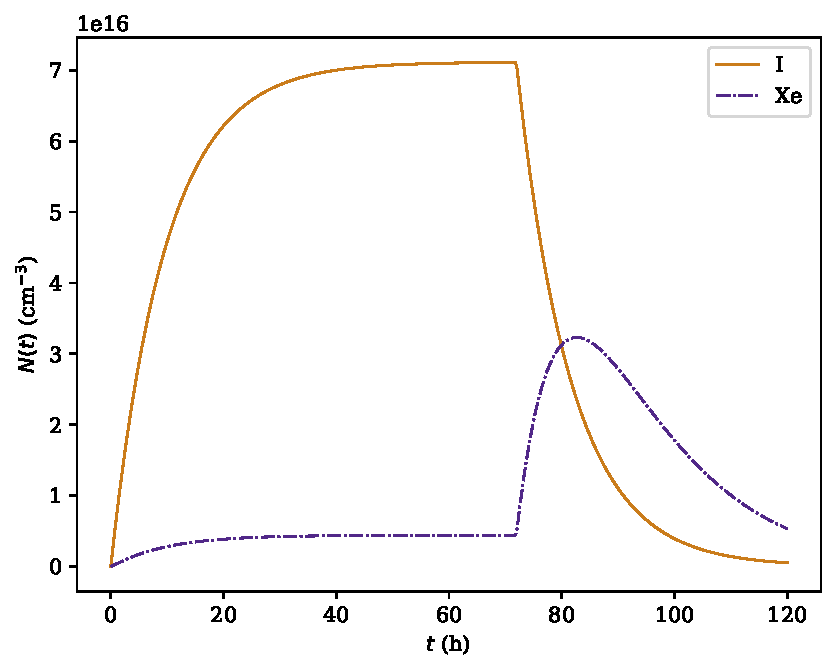
\includegraphics[width=\linewidth]{figures/lesson_22_Xe_transient.pdf}
\end{center}
\figcap{Results of the xenon transient simulation.  Shutdown occurs at 72 h.}

\NEEx{Why does xenon rise after shutdown?}
Setting $\phi=0$ removes direct fission production and neutron
absorption. The balances become
\begin{align*}
 \Alert{\frac{dN_I}{dt}}&=\Alert{-\lambda_I N_I},\\
 \Primary{\frac{dN_{Xe}}{dt}}&=\Primary{-\lambda_{Xe}N_{Xe}}
                              +\Alert{\lambda_I N_I}.
\end{align*}
Iodine continues to feed xenon after the neutron-absorption sink
disappears. Xenon therefore initially rises in this experiment, peaks,
and then decays as the iodine reservoir is exhausted.

\vspace{5pt}

{\bf Ponderable}:
At the xenon peak after shutdown, what relation holds between
$\Alert{\lambda_I N_I}$ and $\Primary{\lambda_{Xe}N_{Xe}}$?
How does the changing xenon inventory alter the control needed for restart?
 
\vspace{5pt}


\Sec{9}{Beyond Xe!}
Here, we've emphasized \nucl{135}{Xe} due to its strong impact 
on reactivity and dynamics.
Other strongly absorbing fission products  are
\begin{itemize}
 \item \nucl{149}{Sm} (see FNRP for a discussion), \nucl{147}{Sm};
 \item \nucl{133}{Cs};
 \item \nucl{147}{Nd}, \nucl{143}{Nd};
 \item \nucl{103}{Rh}.
\end{itemize}
For full production/decay chains of important FPs, see the
\href{https://www-nds.iaea.org/wimsd/fpbchains.htm}{IAEA WIMS fission-product chains}.

\colend


\end{document}
